\documentclass{article}
\usepackage[UTF8]{ctex}
\usepackage{amsmath}
\usepackage{amssymb}
\usepackage{listings}
\usepackage{geometry}
\usepackage{mathabx}
\newcommand{\varparallel}{\mathrel{/\mkern-5mu/}}
\geometry{a4paper,scale=0.8}
\usepackage[colorlinks,linkcolor=blue]{hyperref}
\usepackage{graphicx}
\usepackage{float}
\usepackage{subfigure}
\usepackage{multicol}
\usepackage{enumerate}
\usepackage{enumitem}
\usepackage{pifont}
\usepackage{ulem}
\usepackage{indentfirst}
\usepackage{tikz}
\usepackage{siunitx}
\usepackage[version=4]{mhchem}
\usepackage{chemmacros}
\usepackage{chemfig}
\usepackage{pifont}
\usepackage{url}
\usepackage[framemethod=tikz]{mdframed}
\chemsetup[phases]{pos=sub}
\usetikzlibrary{arrows,shapes,automata,petri,positioning,calc}

\title{ZVMS 4.0.0 用户文档}
\author{7086cmd}
\date{\today}

\begin{document}

\maketitle

ZVMS 是镇海中学的义工管理系统. 该系统的目的是为了方便学生和老师管理义工, 并且提供了一些额外的功能, 例如通知中心, 问题反馈等.

该文档为方便用户使用 ZVMS 而编写. 该文档的目的是为了让用户更好地了解 ZVMS 的功能, 并且更好地使用 ZVMS. 因此, 使用中文编写.

该文档的目录如下:

\tableofcontents

\section{用户管理}

\subsection{用户登录}

通过地址 \texttt{https://v4.zvms.site/} 进入 ZVMS 平台后, 若未登录, 则自动跳转至登录界面. (如图 \ref{fig:login})

\begin{figure}[H]
  \centering
  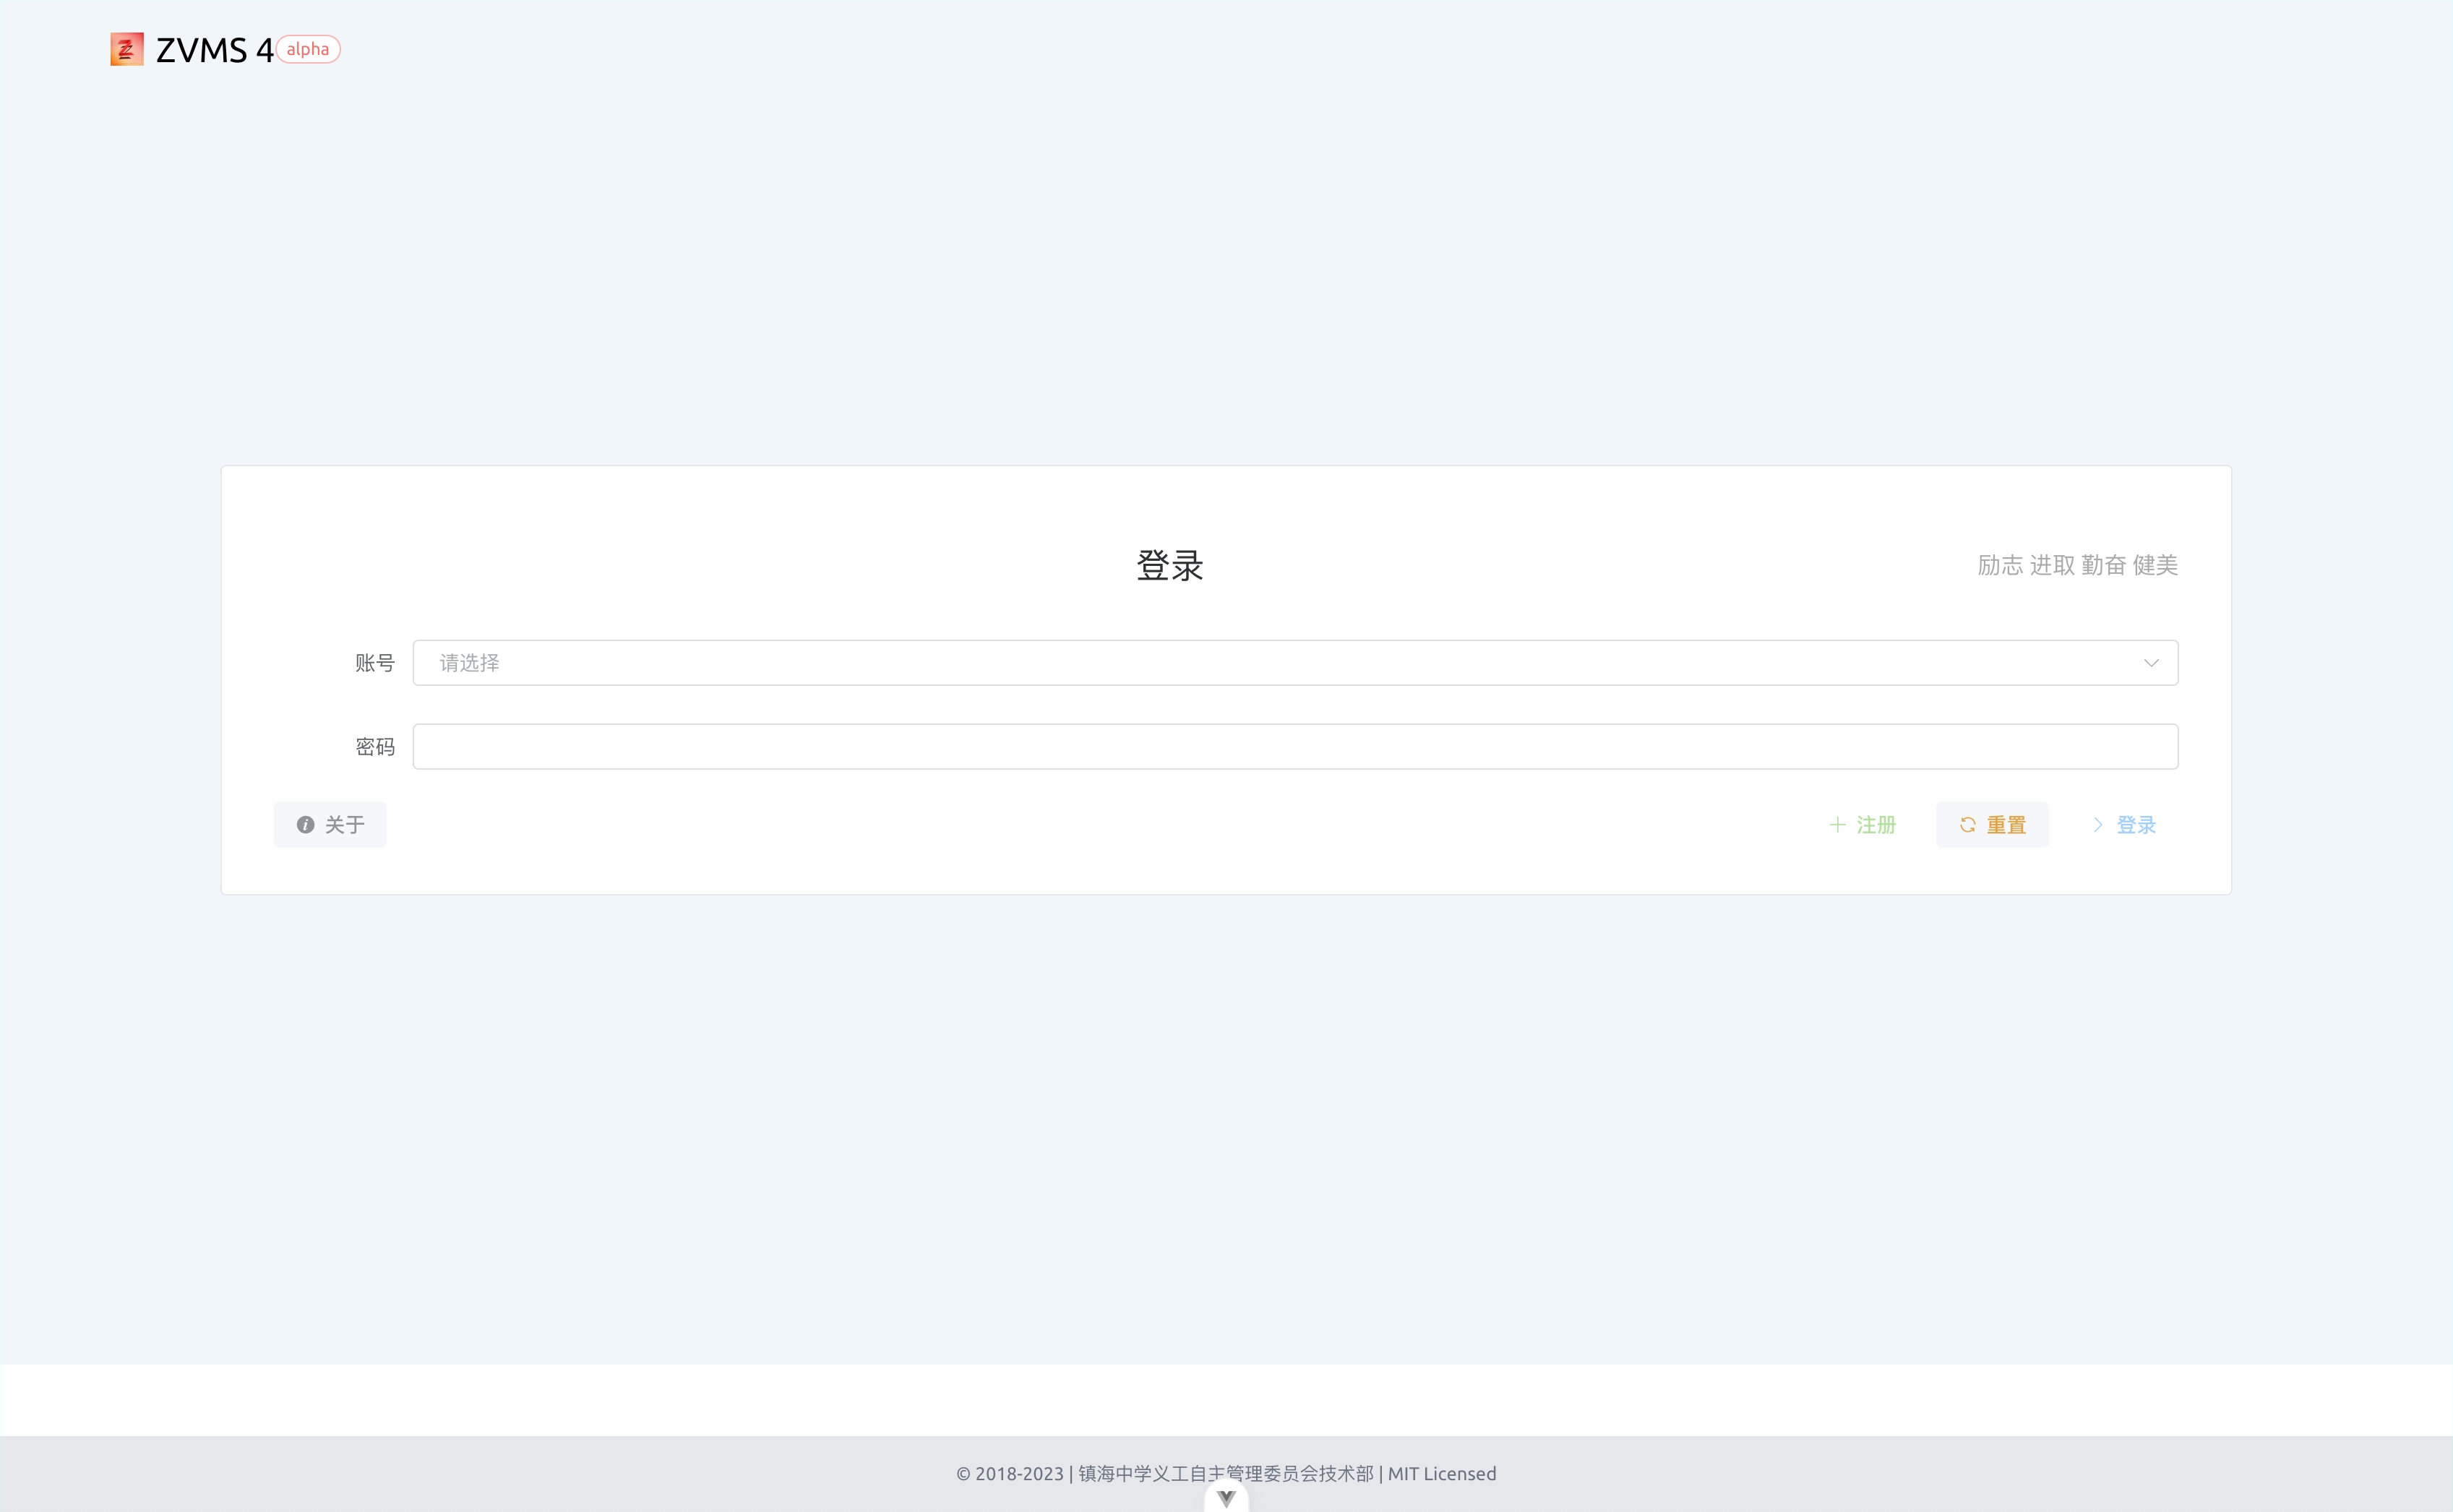
\includegraphics[width=0.8\textwidth]{../assets/image-20240303151532382.png}
  \caption{登录界面}
  \label{fig:login}
\end{figure}

当学号输入至 $6$ 位后, 系统将自动通过数据库检索. 您可以选择您的姓名.

\begin{figure}[H]
  \centering
  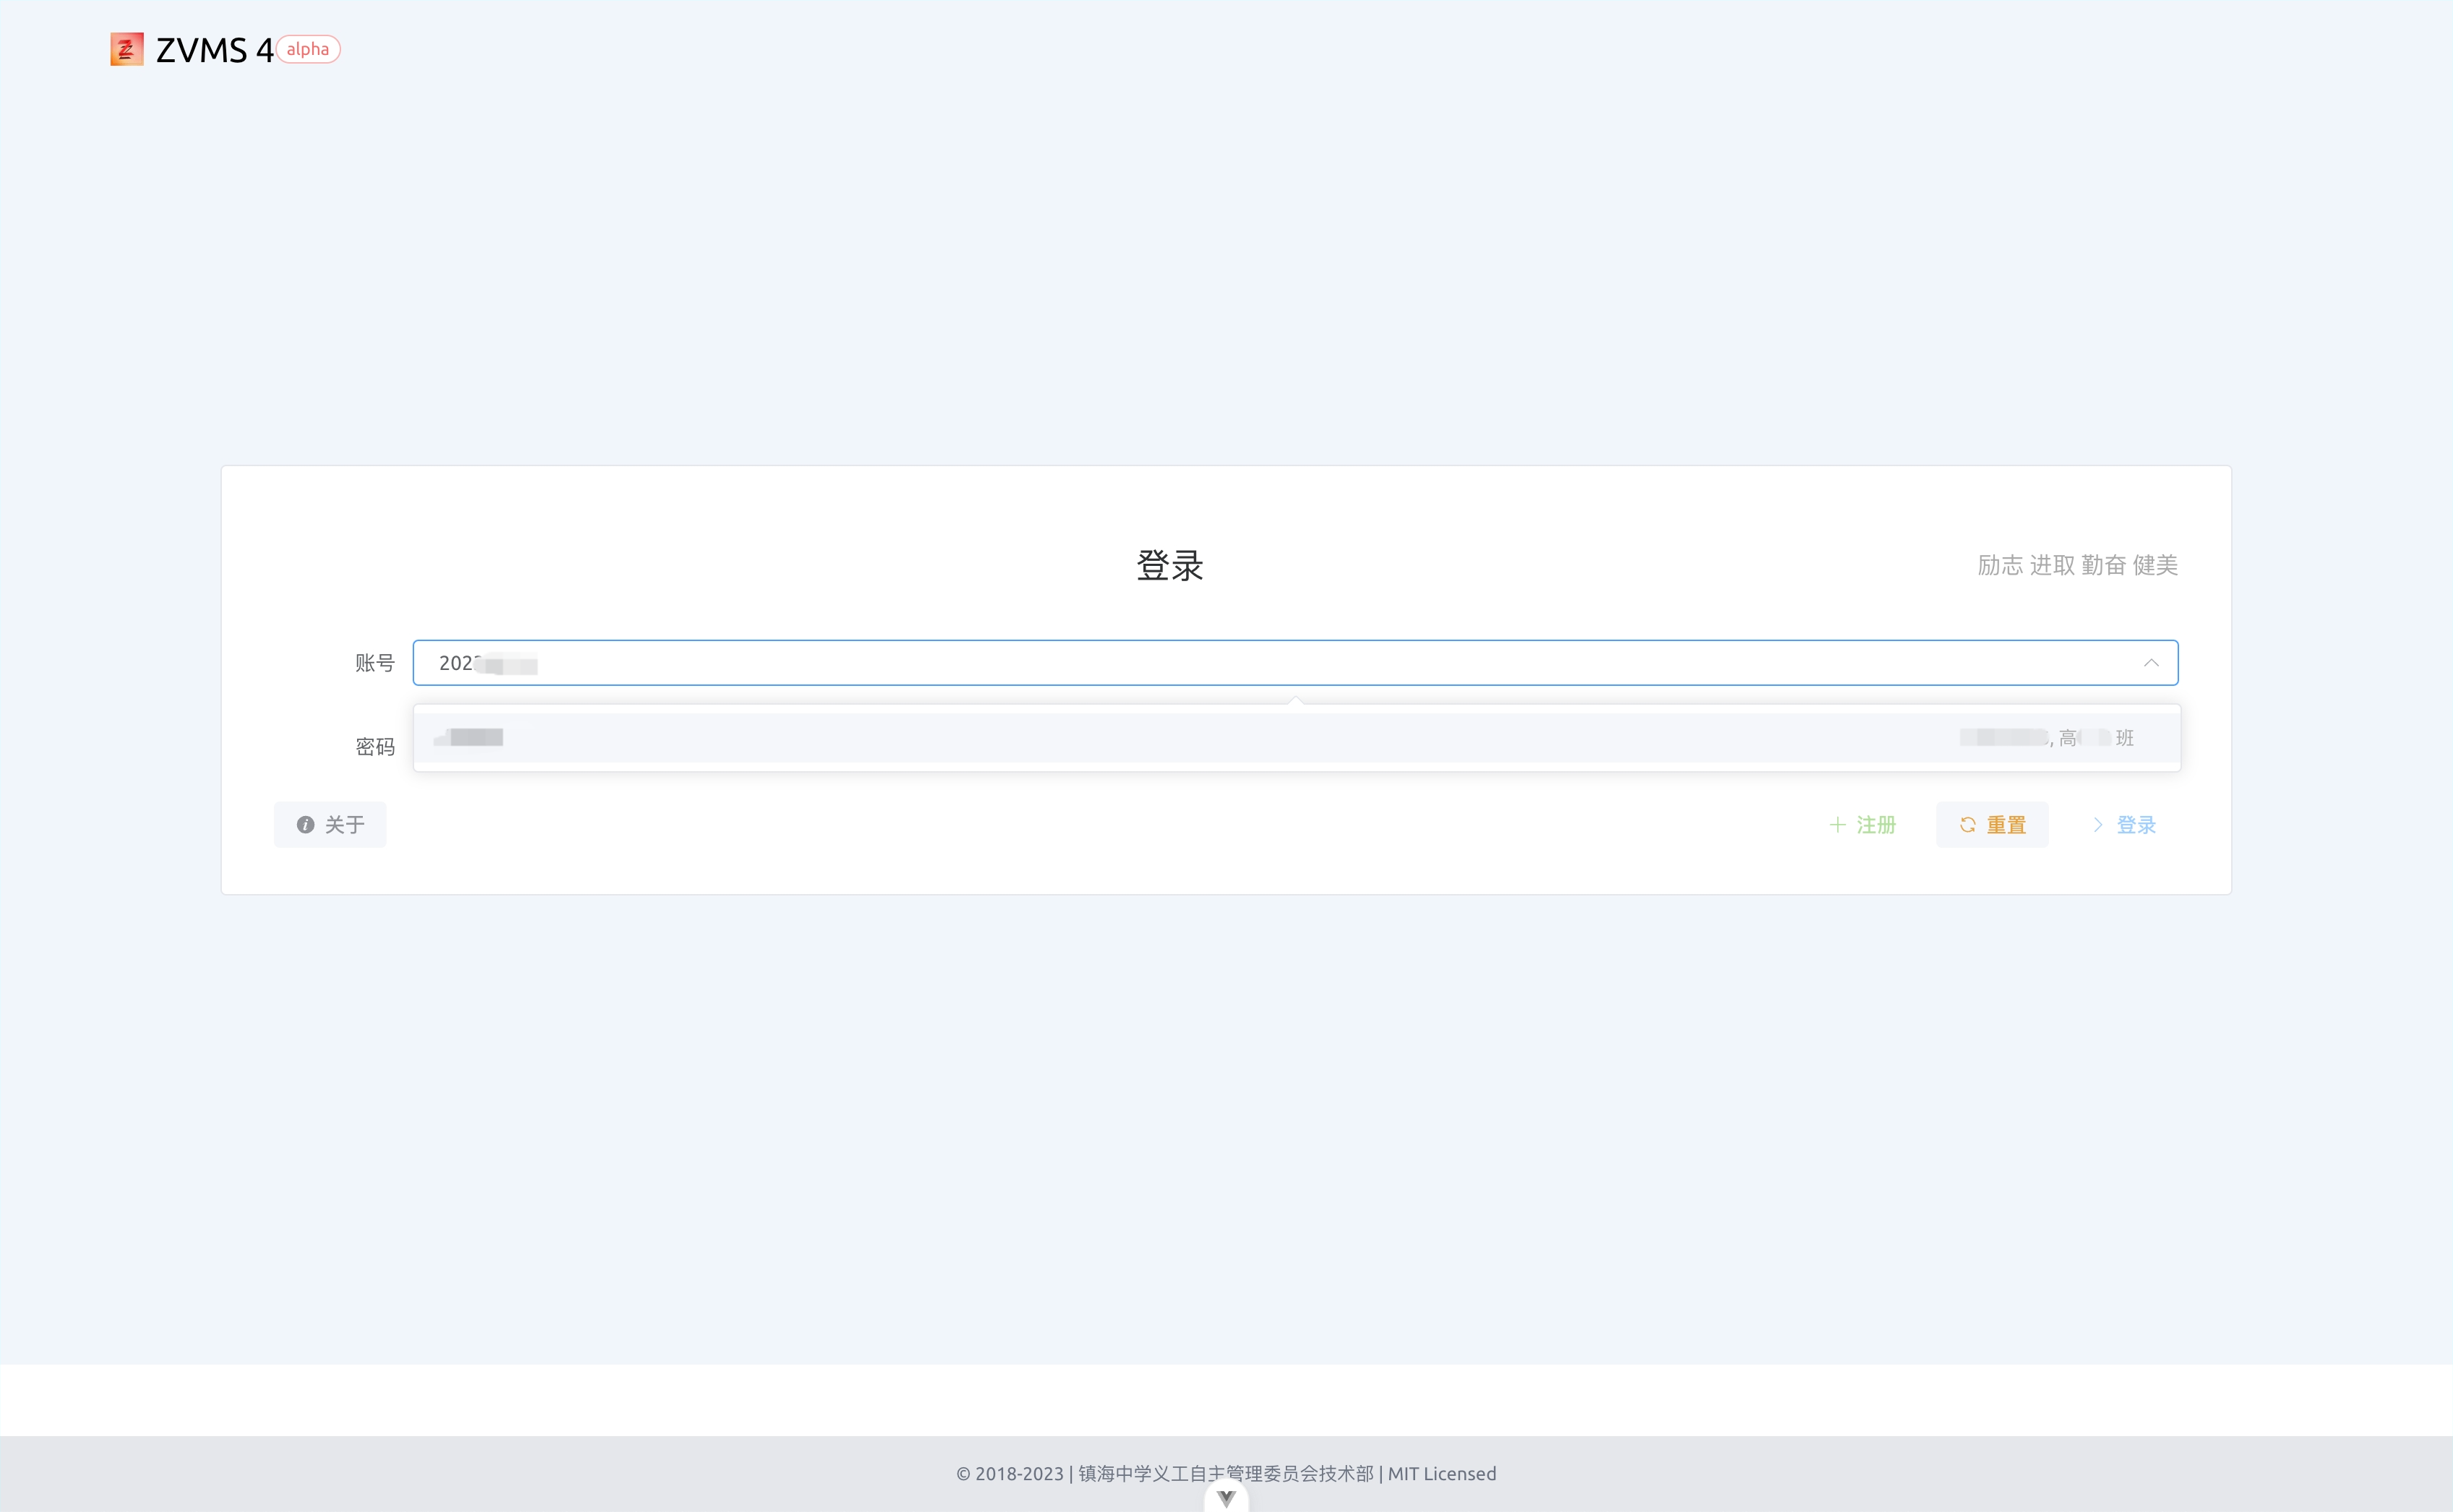
\includegraphics[width=0.8\textwidth]{../assets/image-20240303151823285.png}
  \caption{学号检索}
  \label{fig:search}
\end{figure}

随后, 输入您的学号作为初始密码, 即可登录至平台. 如果中途出现了 \texttt{404 Not Found}, 请关闭页面后重新进入.

\subsection{主页}

在主页中, 平台将会显示您的部分个人信息, 包括您的姓名, 学号, 班级, 以及义工时间. 义工时间的 ``折算'' 是指根据义工管理细则中的 ``溢出机制'' 进行计算后的结果. 您可以切换开关来决定是否显示, 但这不会影响您的义工时间.

\begin{mdframed}
  \fangsong
  溢出机制。若校内义工时间已满,超出的部分按三分之一折算进校外义工时间,总的溢出时长不超过6小时(四舍五入)。
  \hfill \textit{义工管理细则}
\end{mdframed}

\begin{figure}[H]
  \centering
  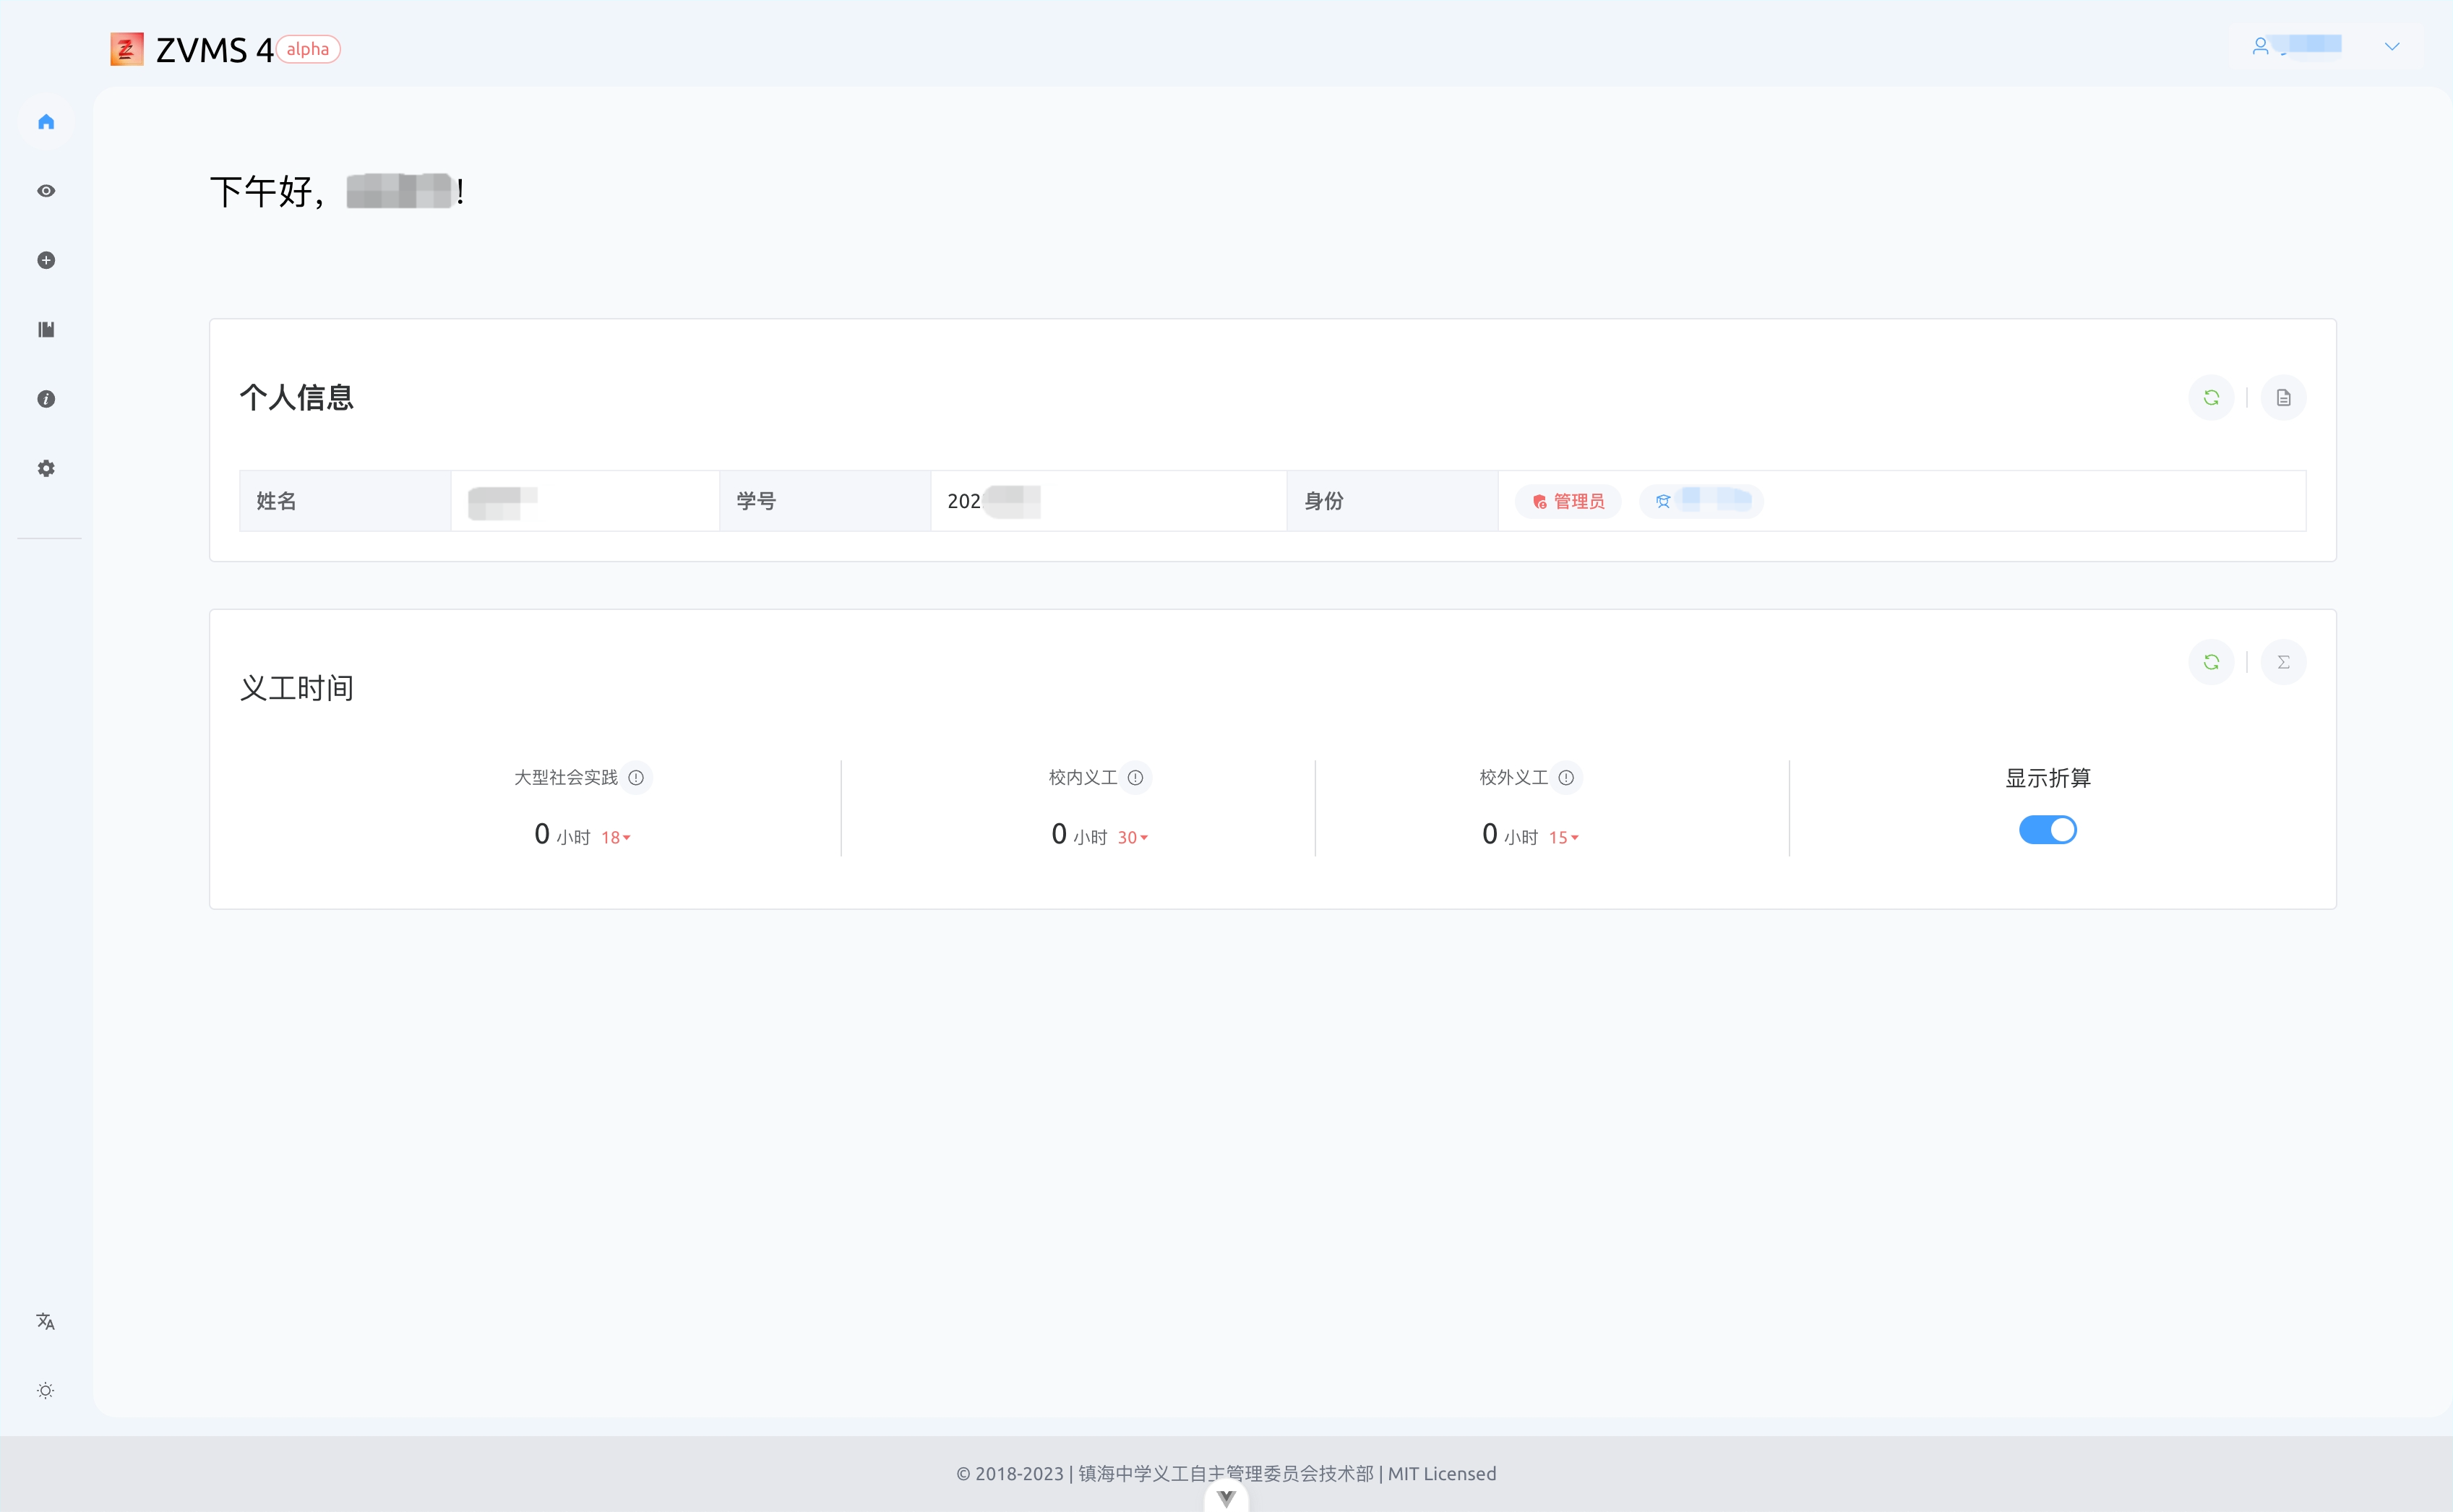
\includegraphics[width=0.8\textwidth]{../assets/image-20240303152245767.png}
  \caption{主页}
  \label{fig:home}
\end{figure}

右上角的下拉菜单中预置了 4 个功能: 问题反馈, 通知中心, 修改密码以及退出登录.

\subsubsection{问题反馈}

问题反馈不在平板上呈现.

\begin{enumerate}
  \item 如果是技术相关的问题, 请在 \texttt{GitHub} 上提出 \texttt{issue}:
  \begin{itemize}
    \item 前端仓库: \texttt{https://github.com/zvms/zvms4-frontend};
    \item 后端仓库: \texttt{https://github.com/zvms/zvms4-backend};
    \item 图床模块: \texttt{https://github.com/zvms/skyView}.
  \end{itemize}
  \item 如果是数据库相关问题, 请联系本班团支书反馈.
\end{enumerate}

\subsubsection{通知中心}

见 \ref{sec:notification} 模块.

\subsubsection{修改密码}

为了方便, 修改密码和其他的高危权限的逻辑都是首先验证密码其次进行操作.

然而, 为了安全起见, 所有验证高危权限 (如修改他人密码, 删除数据等) 都需要强密码. 在获取临时的 \texttt{token} 时, 系统若检测到您的密码不符合要求, 则会禁用提交按钮, 并在输入框下方显示错误信息.

\begin{figure}[H]
  \centering
  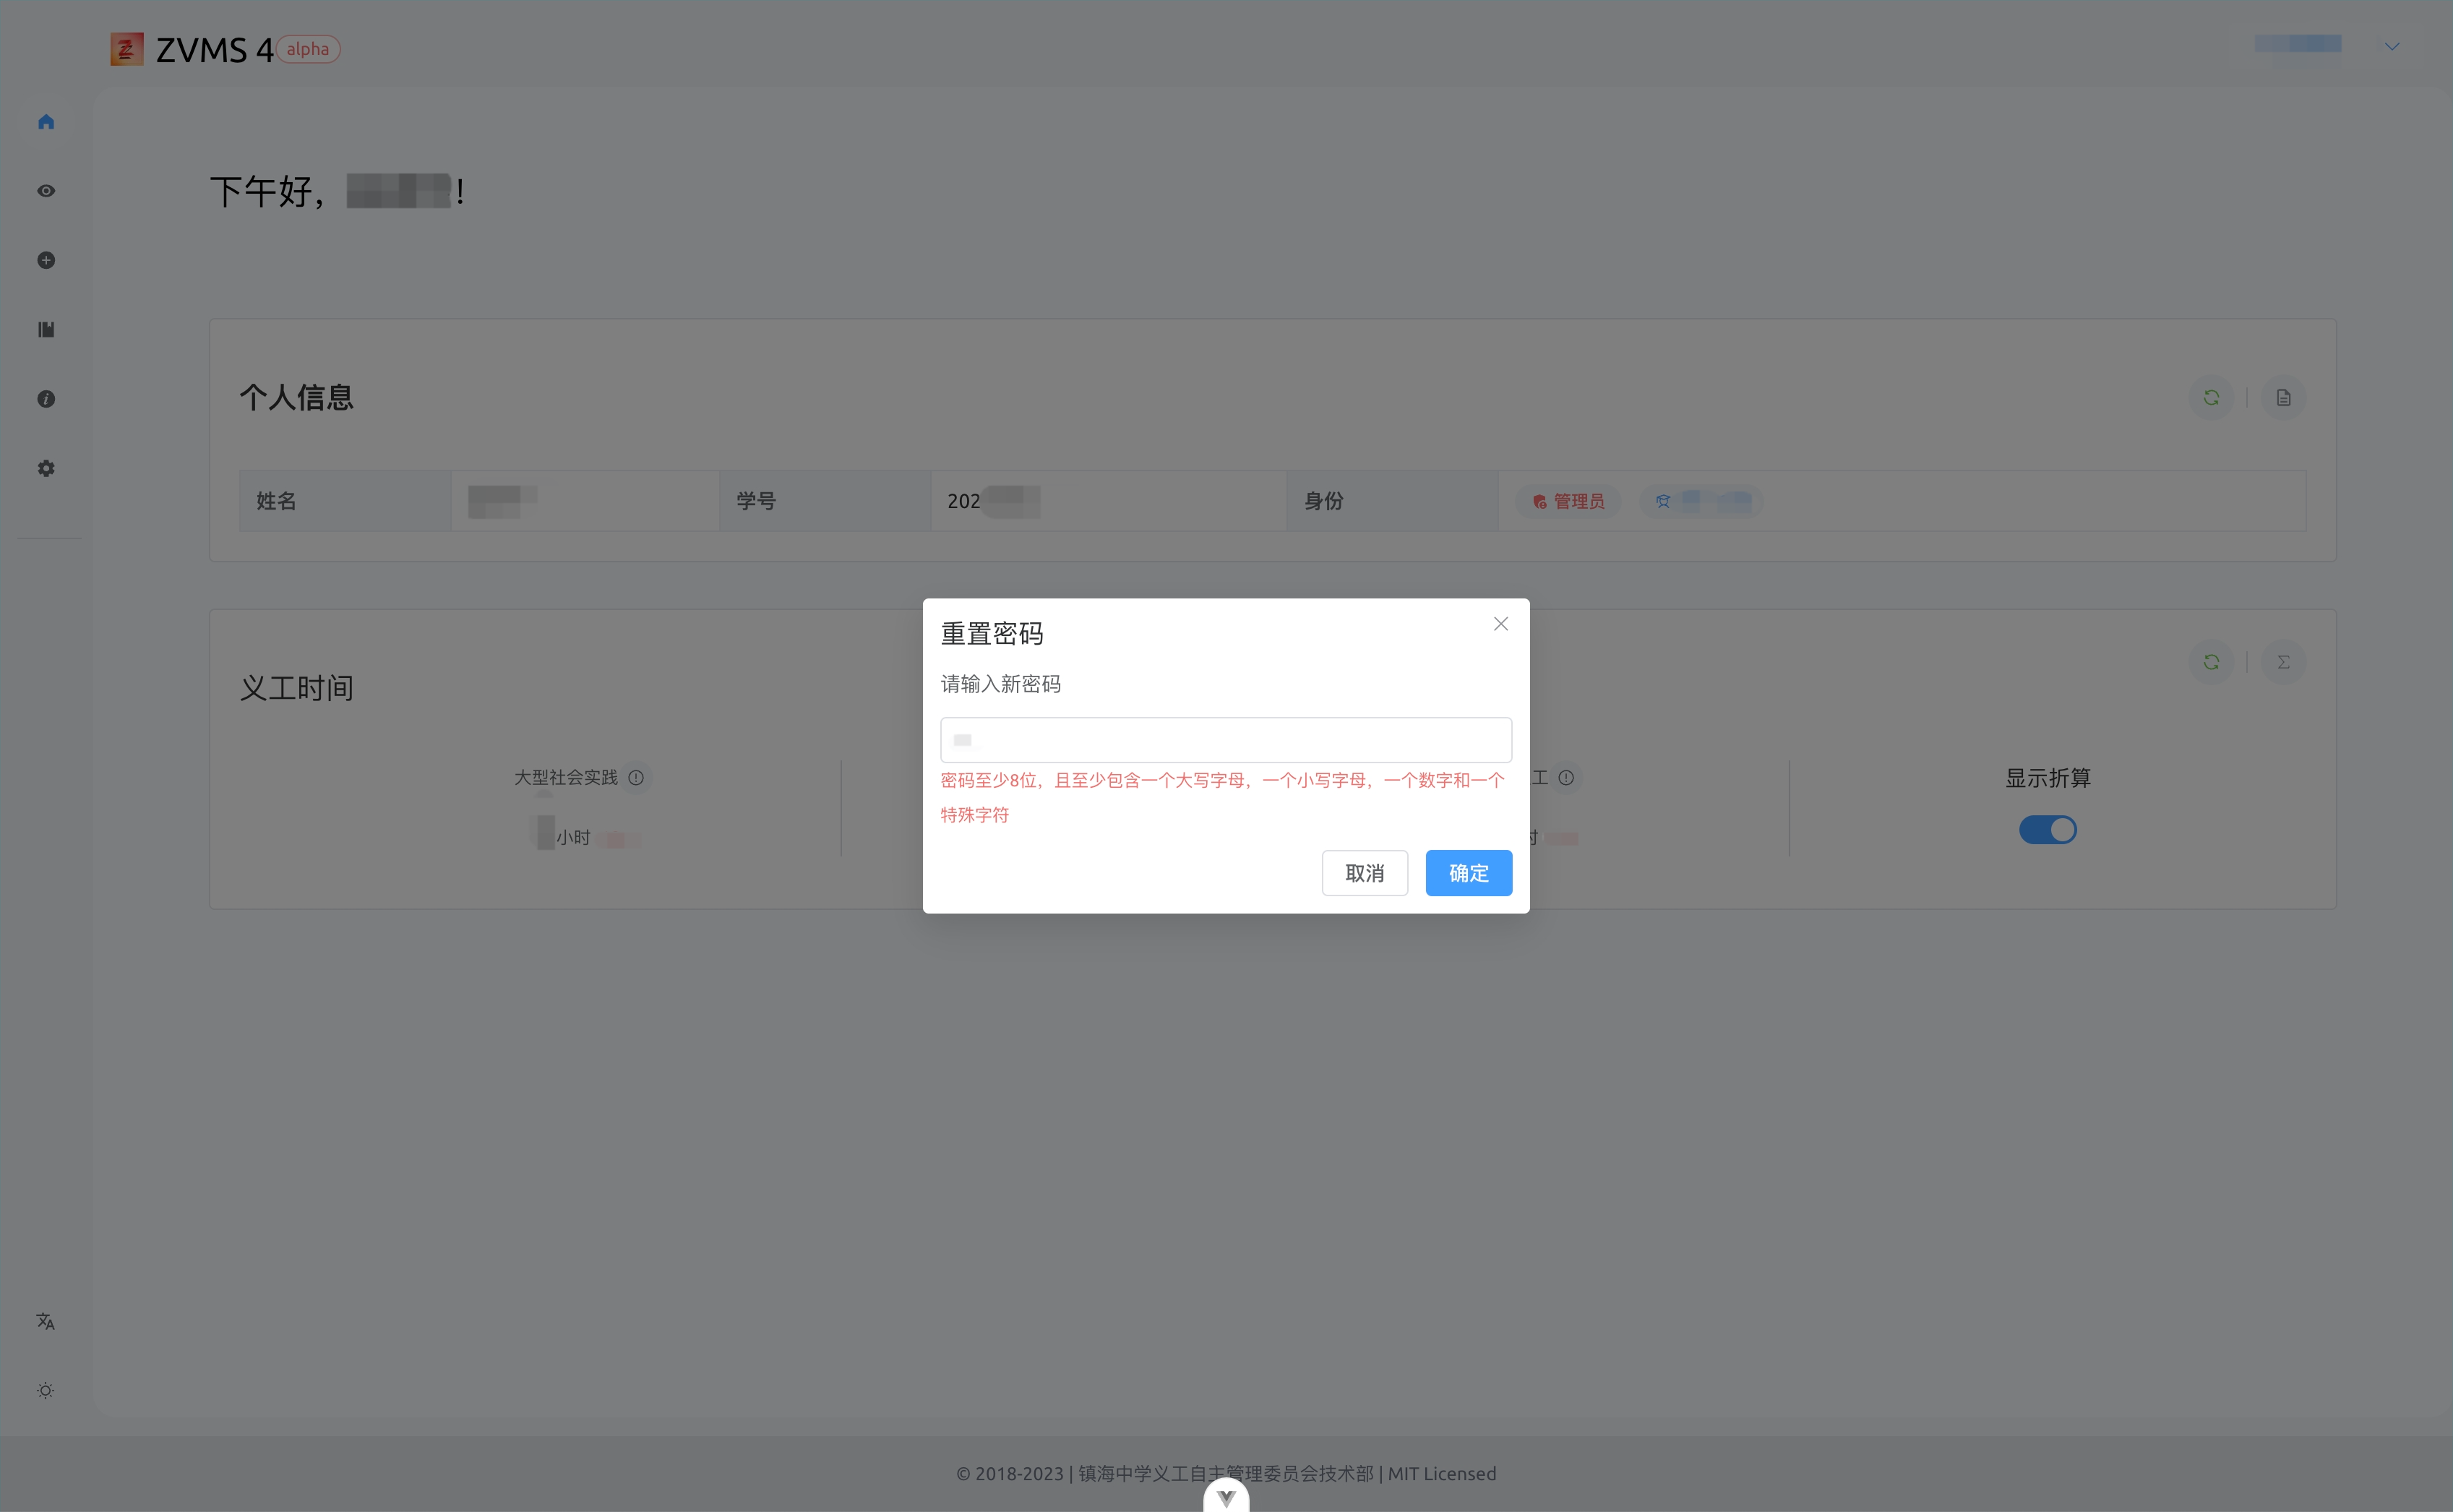
\includegraphics[width=0.8\textwidth]{../assets/image-20240303153008248.png}
  \caption{修改密码}
  \label{fig:change-password}
\end{figure}

当您选择 ``修改密码'' 时, 您需要首先输入您的初始密码. 若您已经修改好了密码却仍想要修改, 则输入修改前的密码. 如果没有任何反应, 上方的加载条也没有显示, 则大概率认为您的密码输入错误.

输入成功后, 您可以输入新的密码. 请注意, 该密码需要为强密码, 至少 8 个字符, 且必须包含至少 1 个大写字母, 1 个小写字母, 1 个数字和 1 个特殊字符.

若修改成功, 则重新登录. 您最好关闭页面后重新进入.

\subsubsection{退出登录}

无须多言. 若退出登录后未到达登录界面, 请清除浏览器缓存后重新进入.

\section{义工管理}

义工管理是 ZVMS 平台的本职工作. 使用 ZVMS, 您可以优雅地管理学校的义工和自己的义工时间.

\subsection{义工列表}

义工列表中, 共有 $2 + 3$ 个选项. 其中, ``我的'' 选项对于具有学生权限的账号开放, ``班级'' 选项对于具有团支书权限的账号开放, ``校内'' 选项对于具有实践部, 审计部, 管理员或监督员权限的账号开放.

\begin{figure}[H]
  \centering
  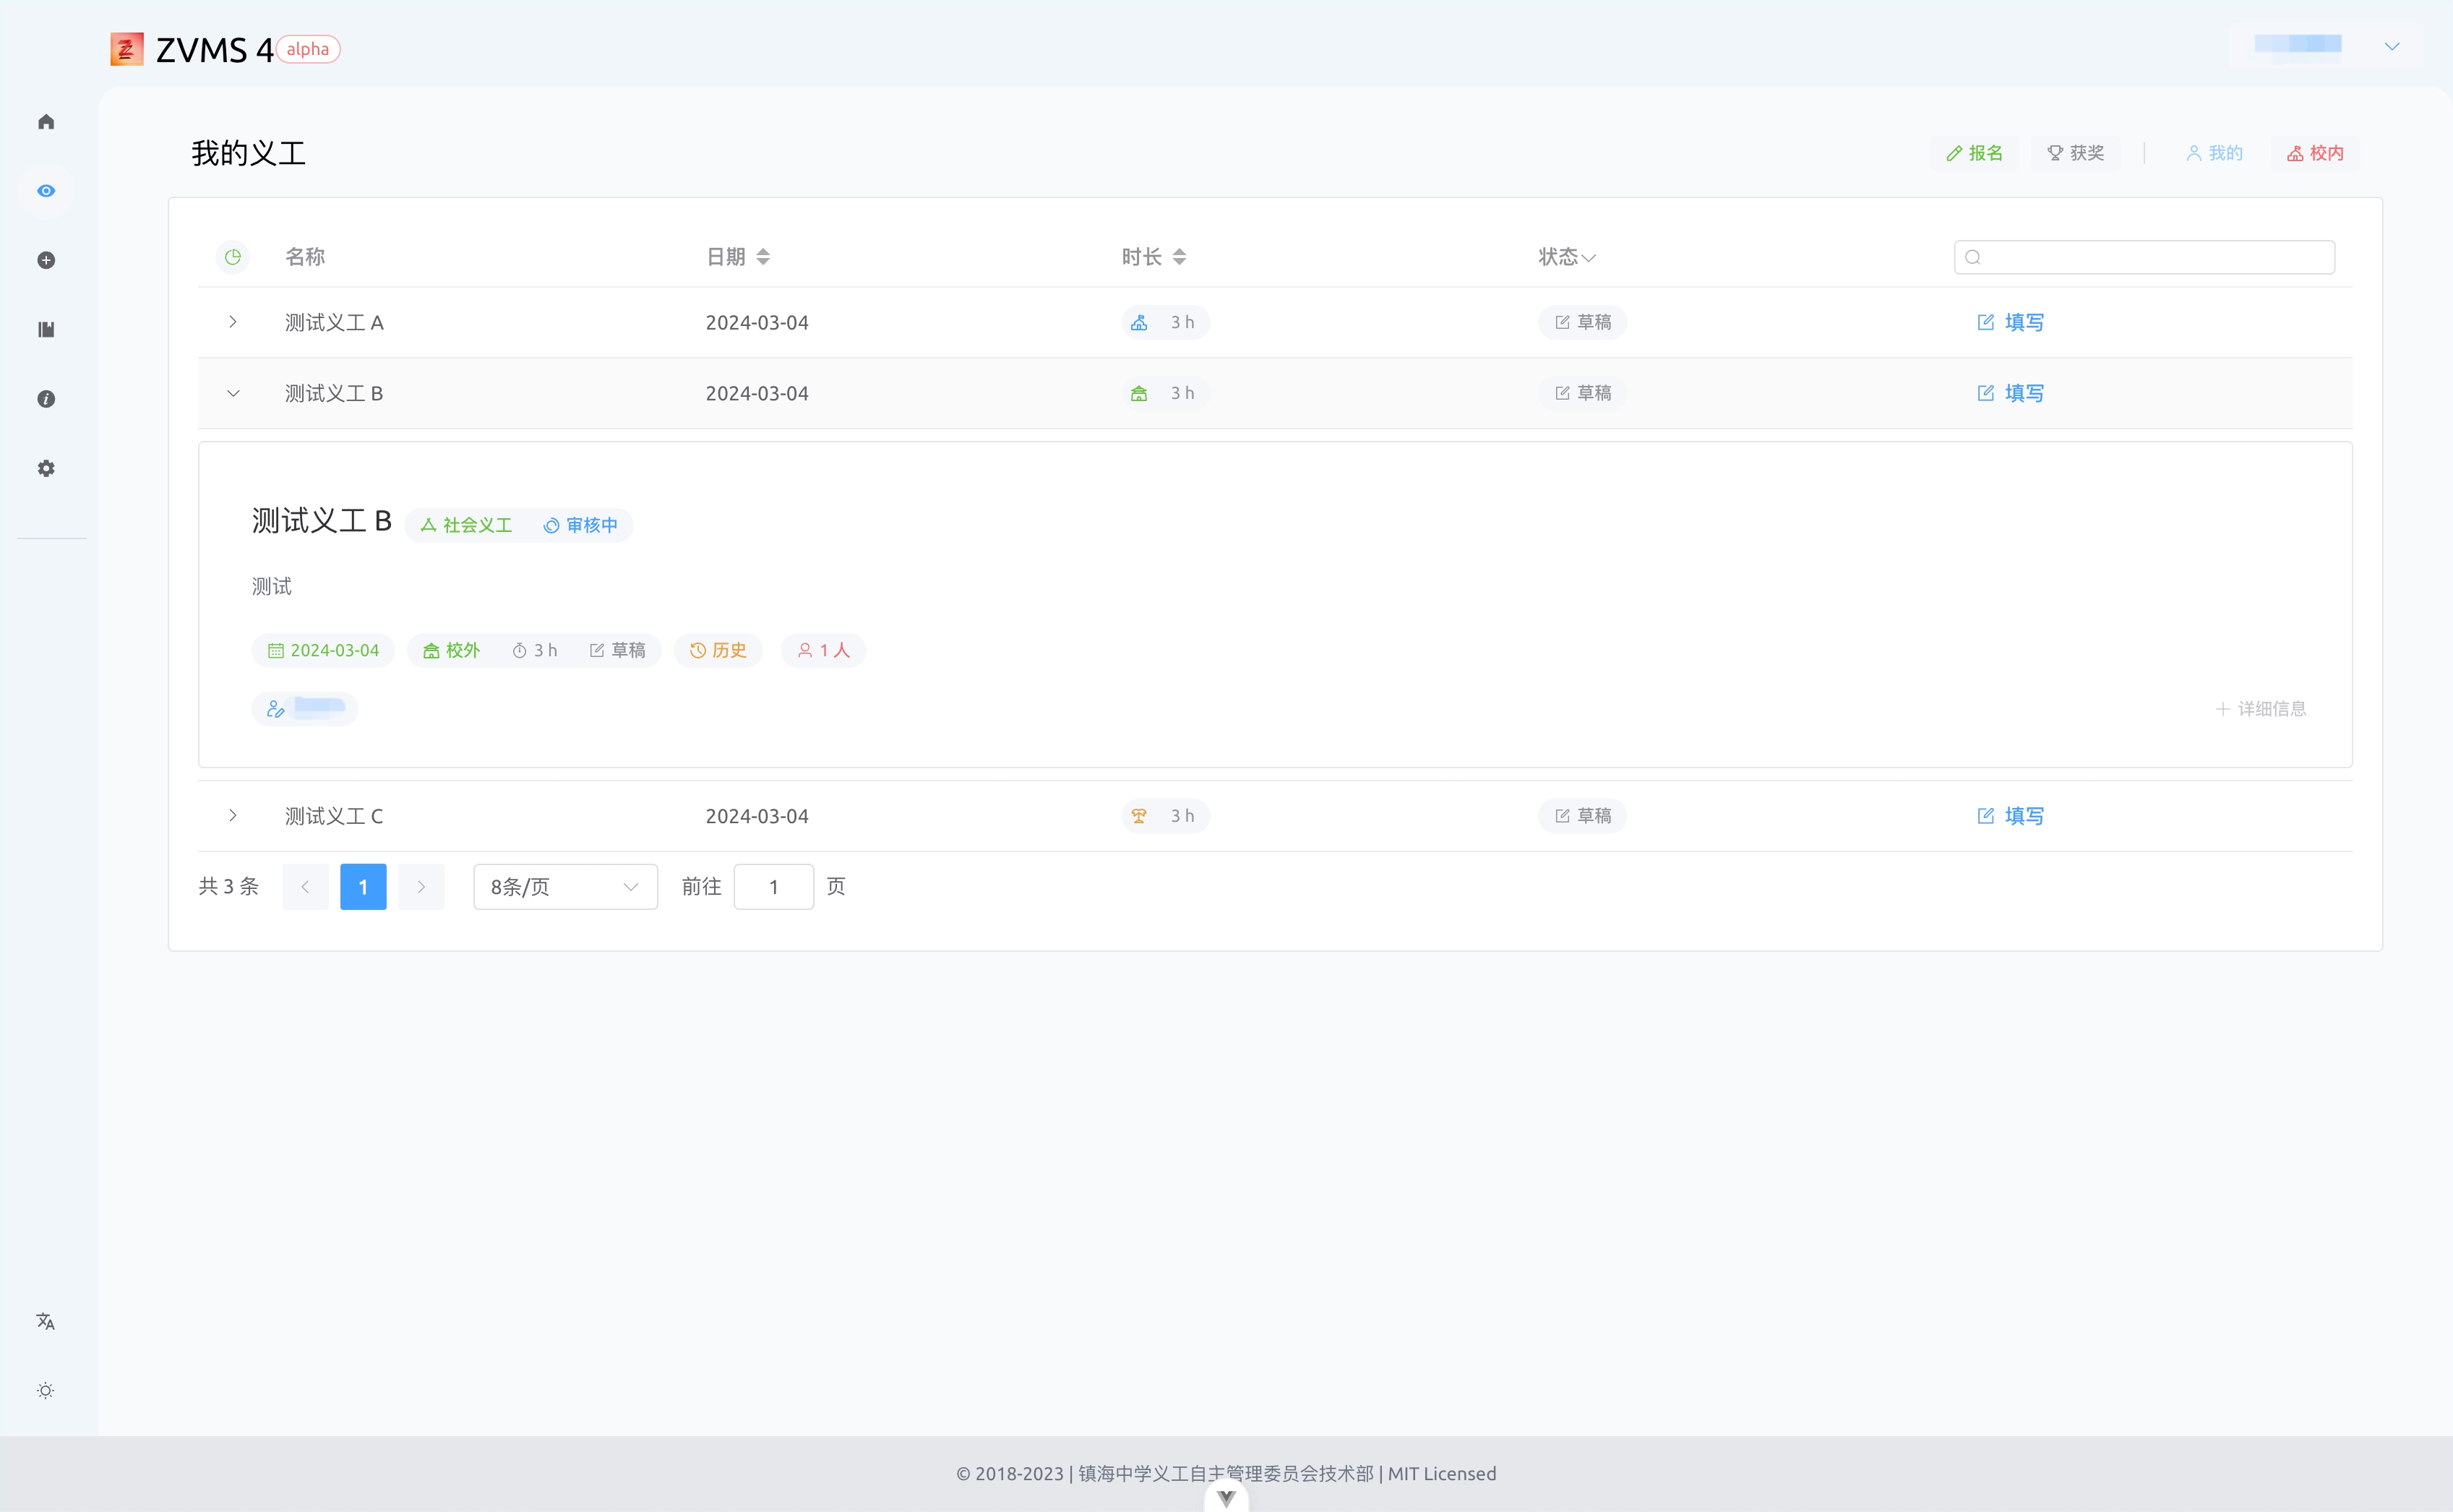
\includegraphics[width=0.8\textwidth]{../assets/image-20240303153534228.png}
  \caption{义工列表}
  \label{fig:volunteer-list}
\end{figure}

\subsection{义工感想}

\subsubsection{感想填写}

在 ``我的'' 界面, 您可以填写您的感想. 其中, 指定义工仅需要填写文字感想, 社会义工需要文字感想和证明图片, 社会实践则需要文字感想和汇报视频 (见相关文件).

\begin{figure}[H]
  \centering
  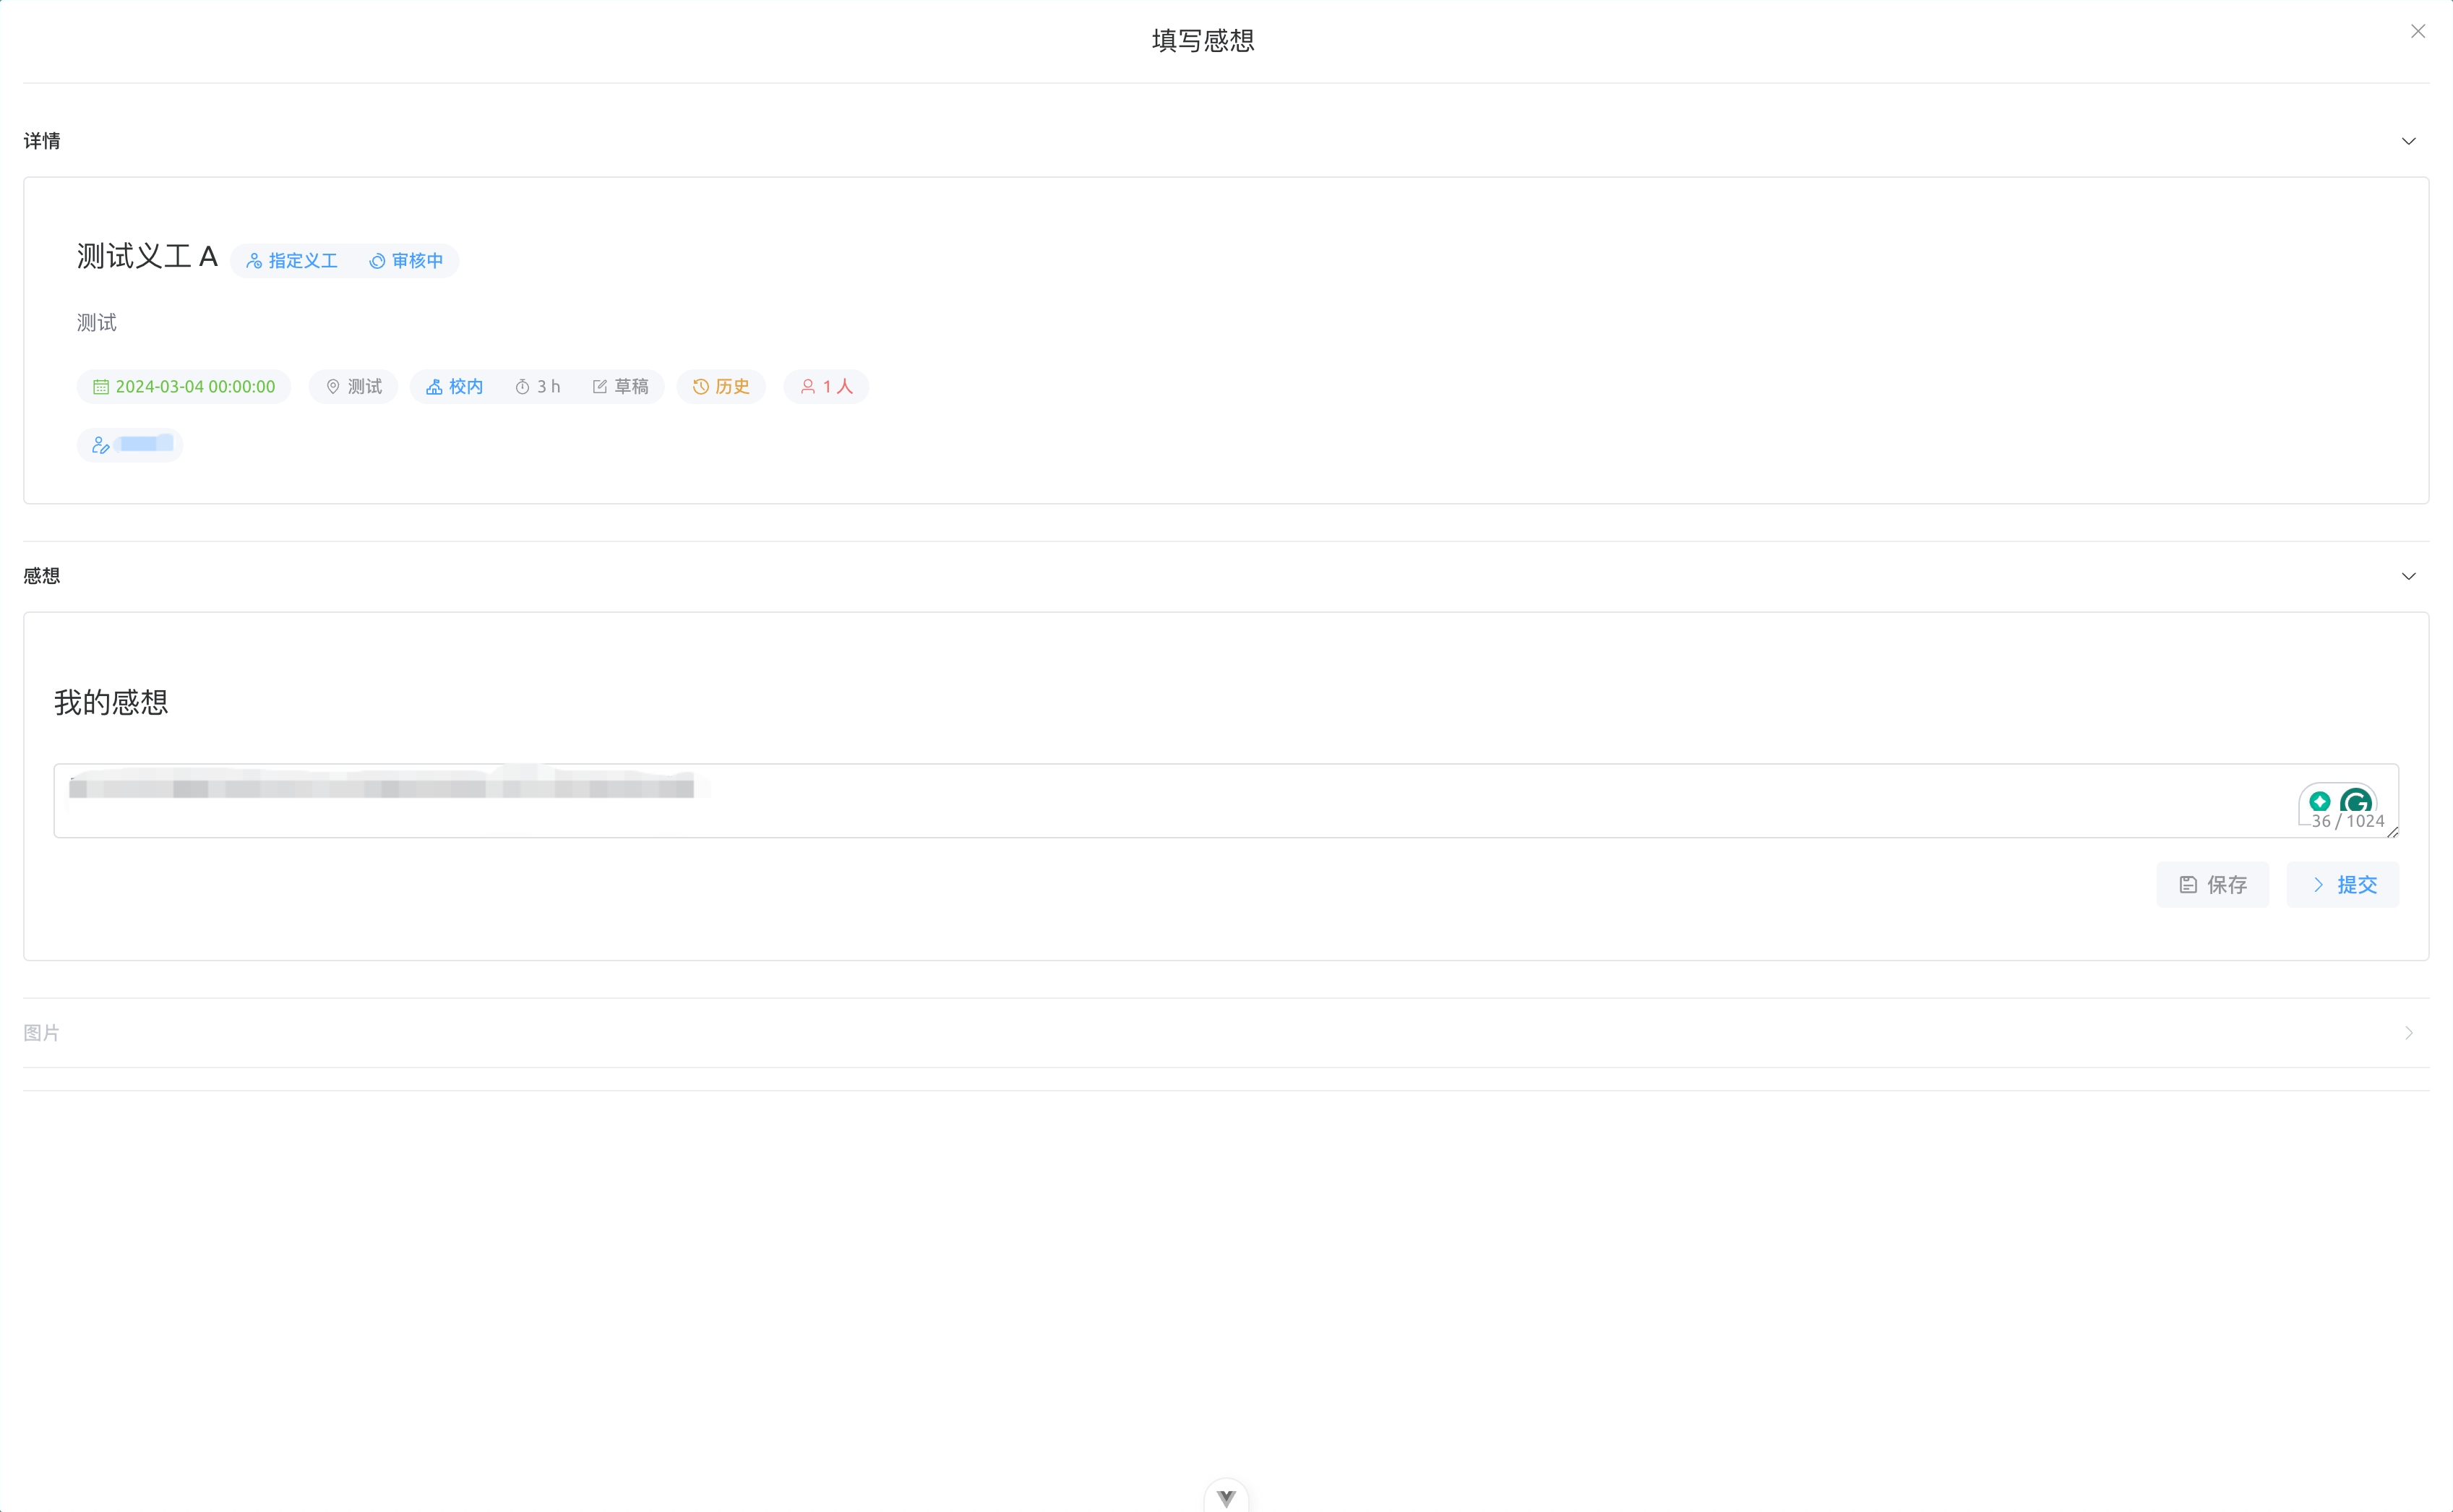
\includegraphics[width=0.8\textwidth]{../assets/image-20240303153939095.png}
  \caption{义工感想填写}
  \label{fig:volunteer-feelings}
\end{figure}

点击单个义工的 ``填写'' 后, 您可以在输入框中写您的感想. 右下角的 ``保存'' 和 ``提交'' 按钮都可以存储您的感想到数据库, 但前者可以随时存储, 后者为提请审批, 根据规定, 需要至少 $30$ 个字才会启用该按钮. 在按钮上方可以看到您目前的字符数. 值得一提的是, 如果您使用英语提交感想, 将会很快达到指定字数, 但也会很快遭到拒绝.

如果是校外义工, 则需要上传图片.

\begin{figure}[H]
  \centering
  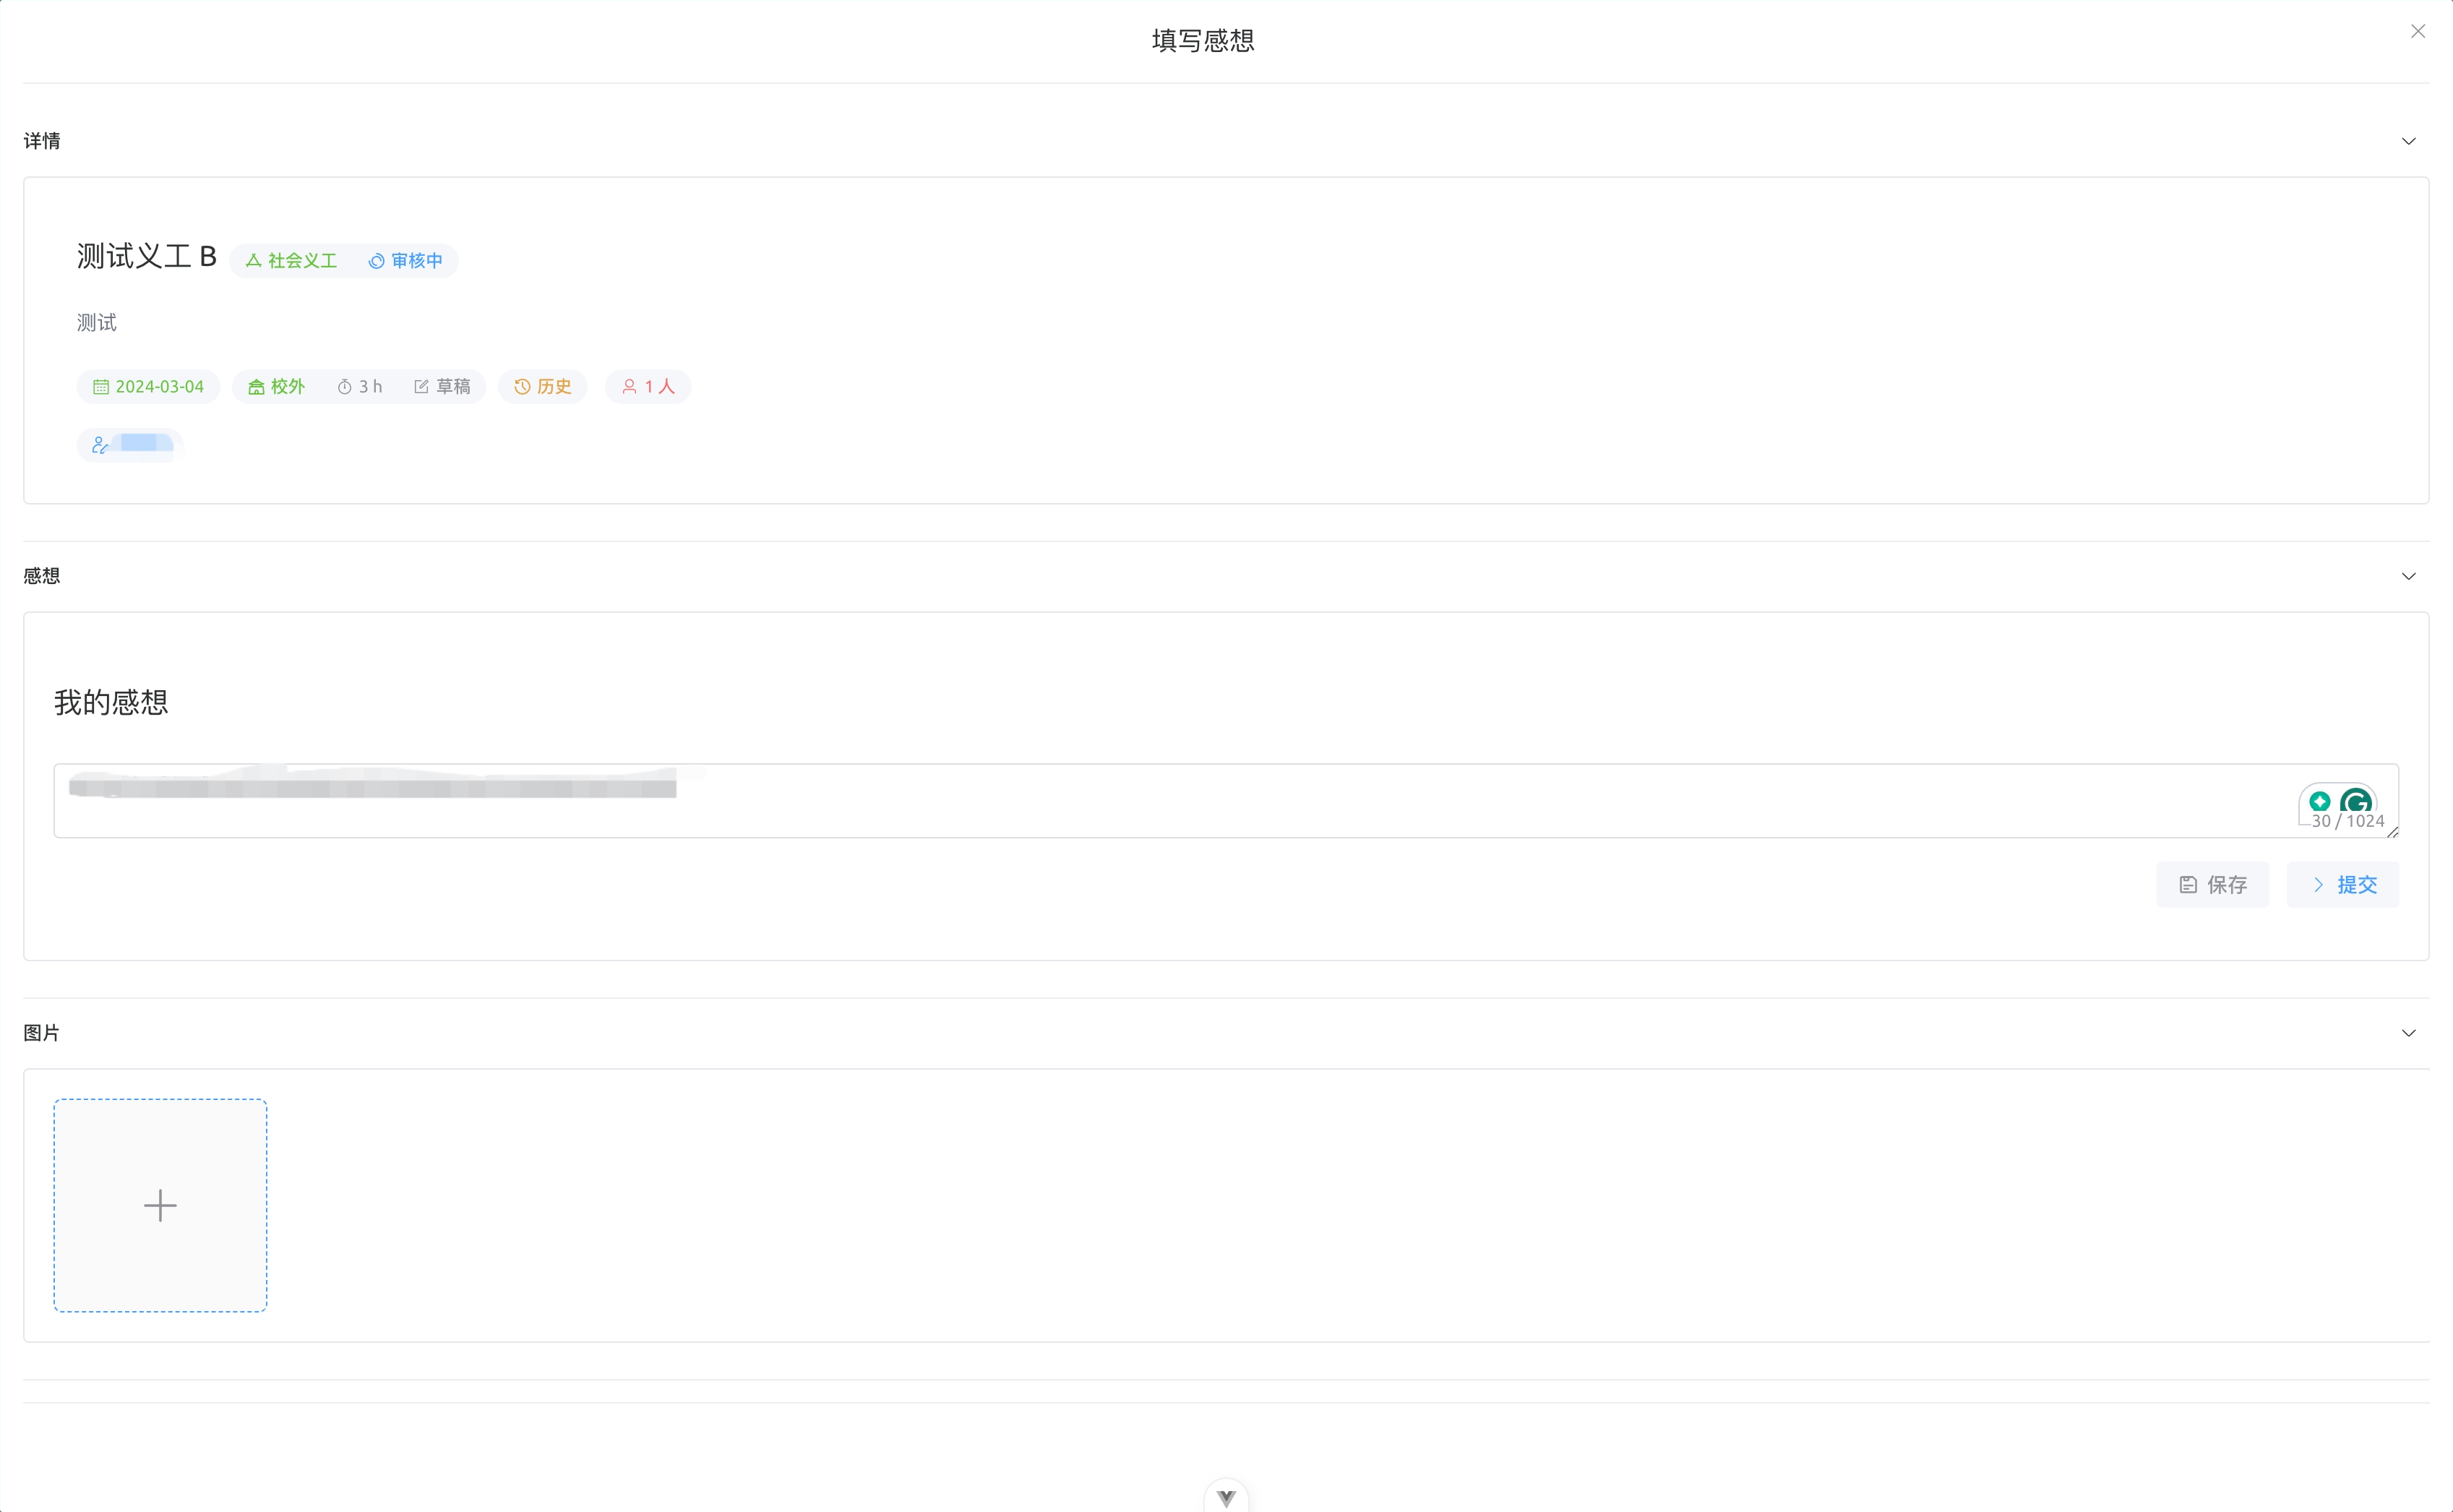
\includegraphics[width=0.8\textwidth]{../assets/image-20240303154235701.png}
  \caption{义工感想填写}
  \label{fig:volunteer-feelings-upload}
\end{figure}

在非学海平板设备, 您可以点击 ``+'' 进行图片上传. 必须为图片格式, 且图片会经过自动审核. 如果包含有政治敏感等元素在内, 将不会被接受. 情节严重可能会上报处理.

您的感想将会直接交由审计部审核. 在该版本中, 初审功能已被删除, 改为一审制.

\subsubsection{义工状态审核}

团支书界面可以审核普通学生创建的社会义工或实践义工, 而实践部或管理员权限账号可以审核所有义工.

\begin{figure}[H]
  \centering
  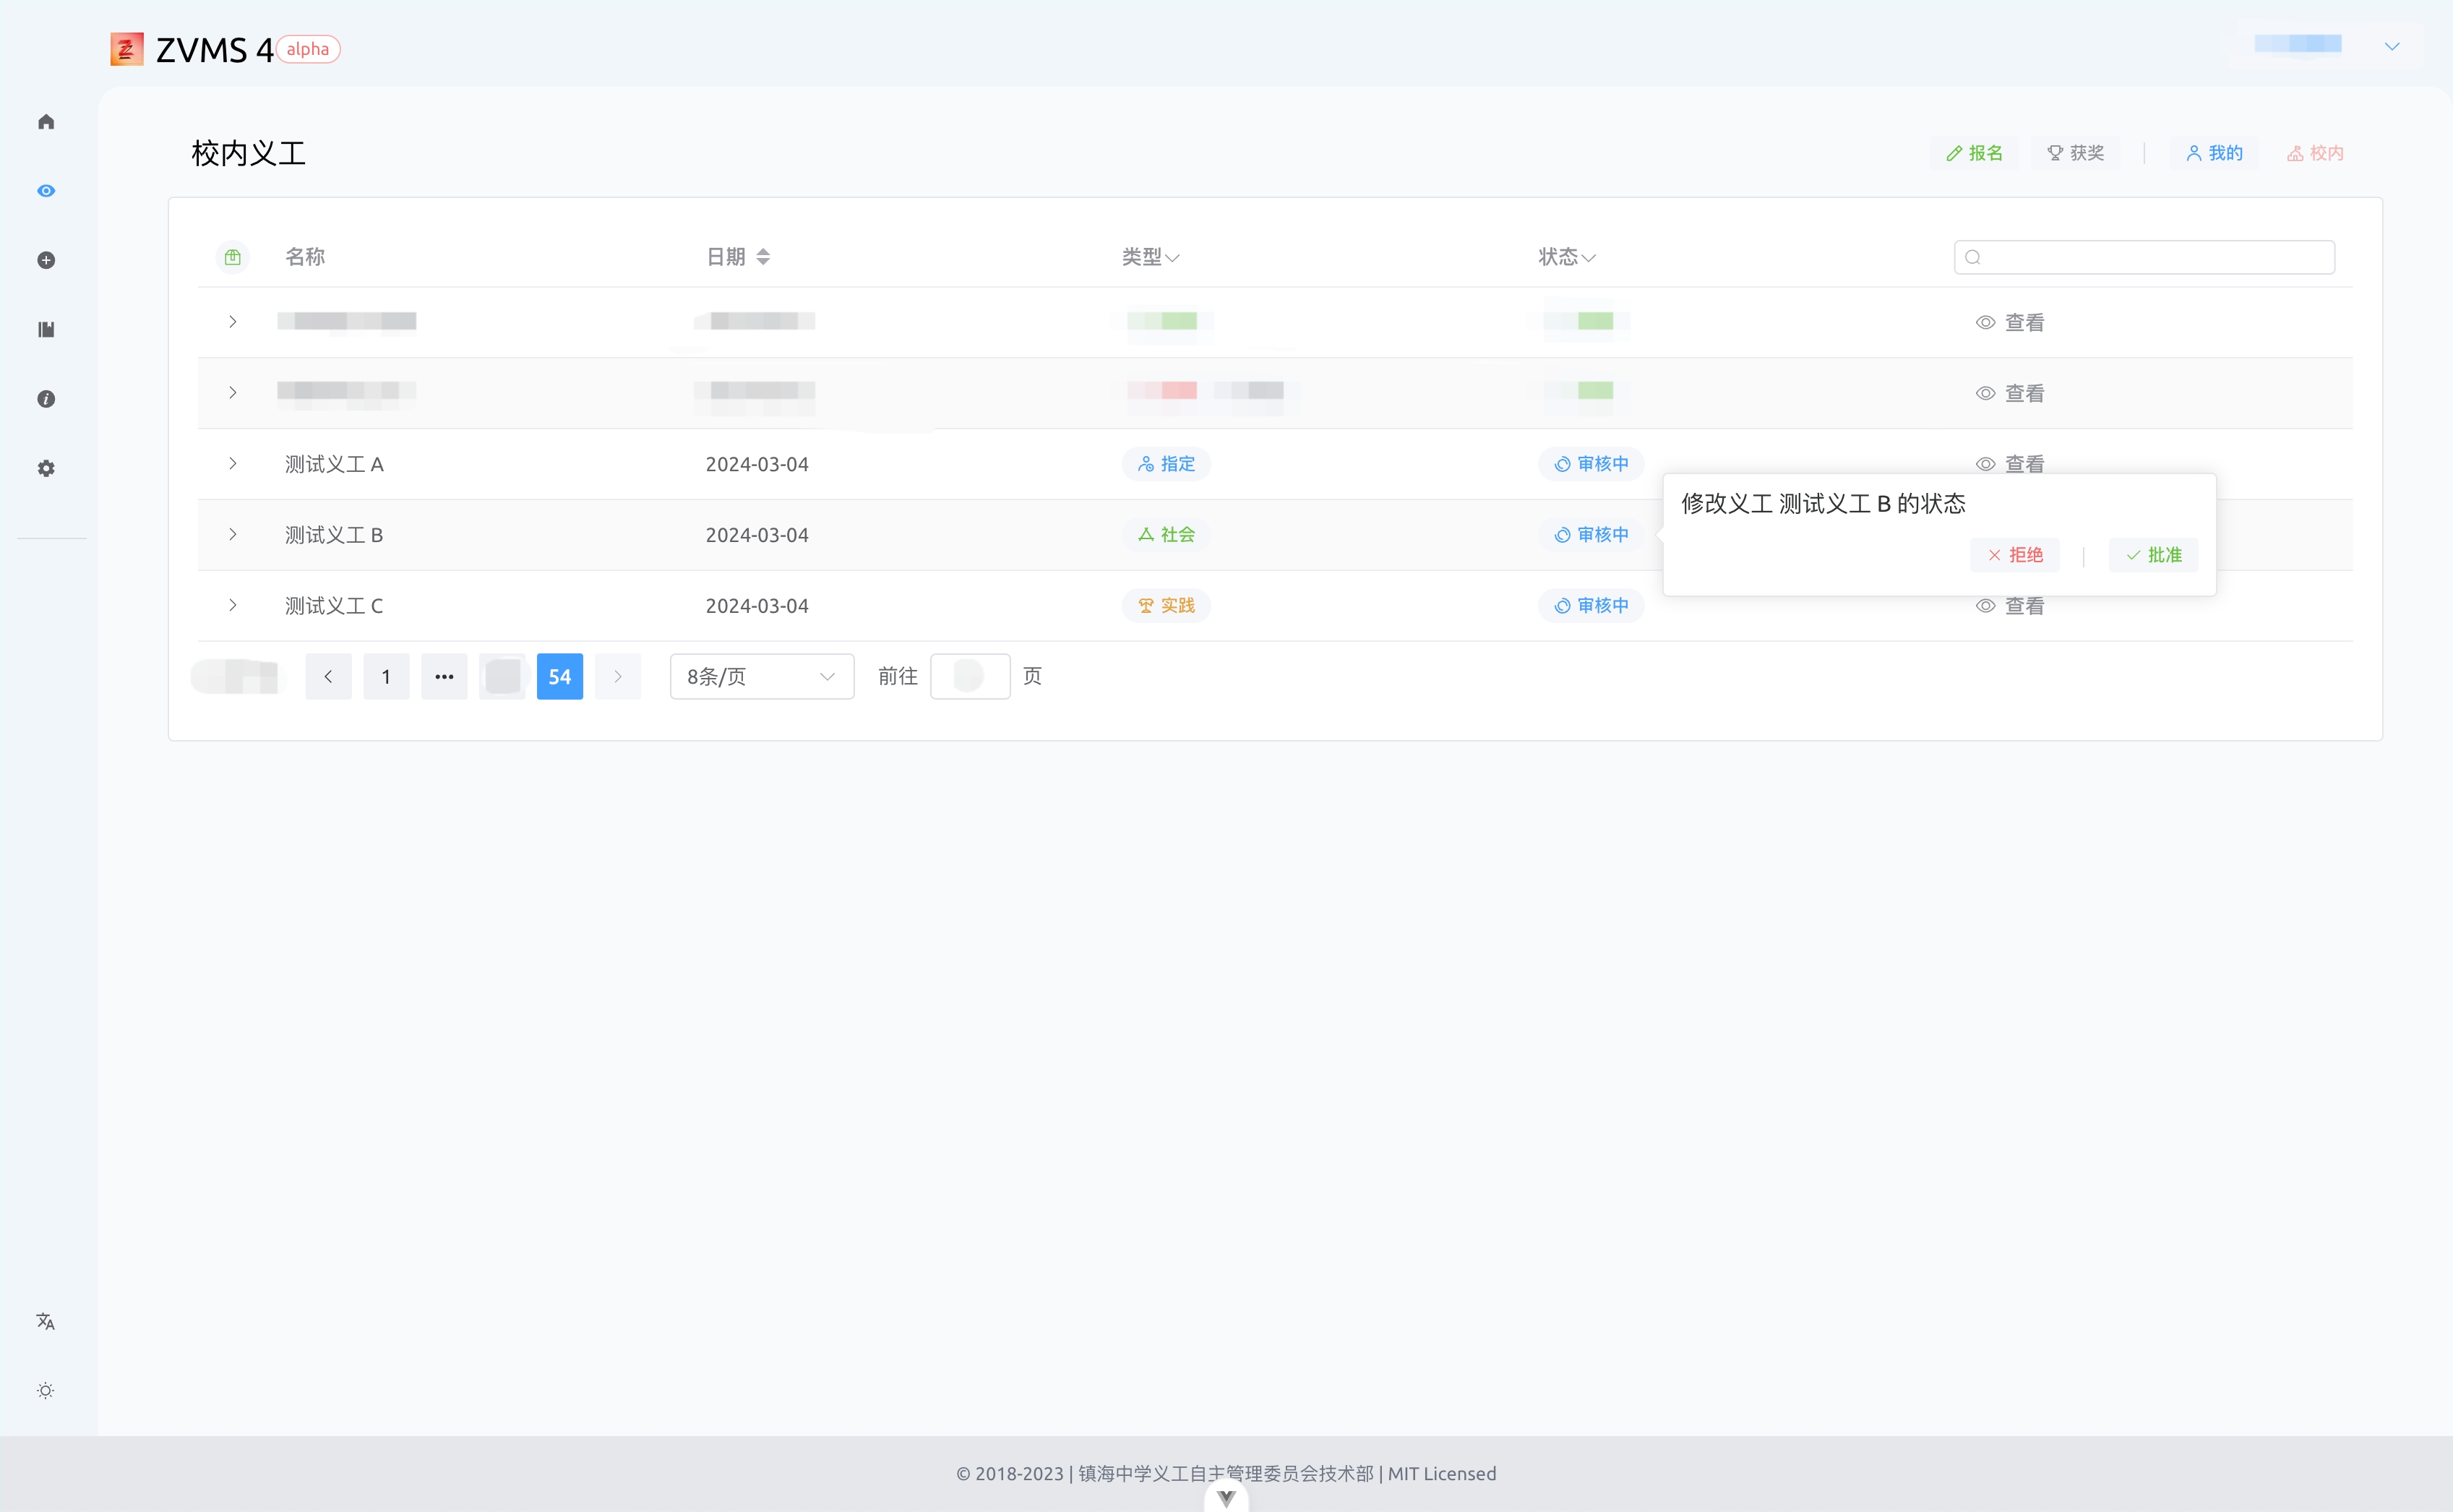
\includegraphics[width=0.8\textwidth]{../assets/image-20240303162112654.png}
  \caption{义工状态审核}
  \label{fig:volunteer-status}
\end{figure}

在 ``班级'' 界面 (对于团支书而言) 或 ``校内'' 界面, 点击 ``审核中'' 的义工状态按钮, 则会跳出修改义工状态的弹出层. 您可以点击 ``拒绝'' 或 ``批准''. 二次确认后, 若拒绝则需要输入密码. 随后会自动刷新, 修改生效. 生效的义工, 生效的感想才可以记入有效时间. 修改后, 状态将不能再次修改.

\subsubsection{审核感想}

具有审核权限的账号可以进入审批感想的页面. 在该页面中, 您可以查看所有人的感想, 并修改 ``审核中'' 的义工感想状态为 ``批准'', ``驳回'' 或 ``拒绝''. 请注意, 被认定为拒绝的义工感想将无法再次填写提交审核. 您需要确定该义工成员存在违纪现象, 不可擅自拒绝.

\begin{figure}[H]
  \centering
  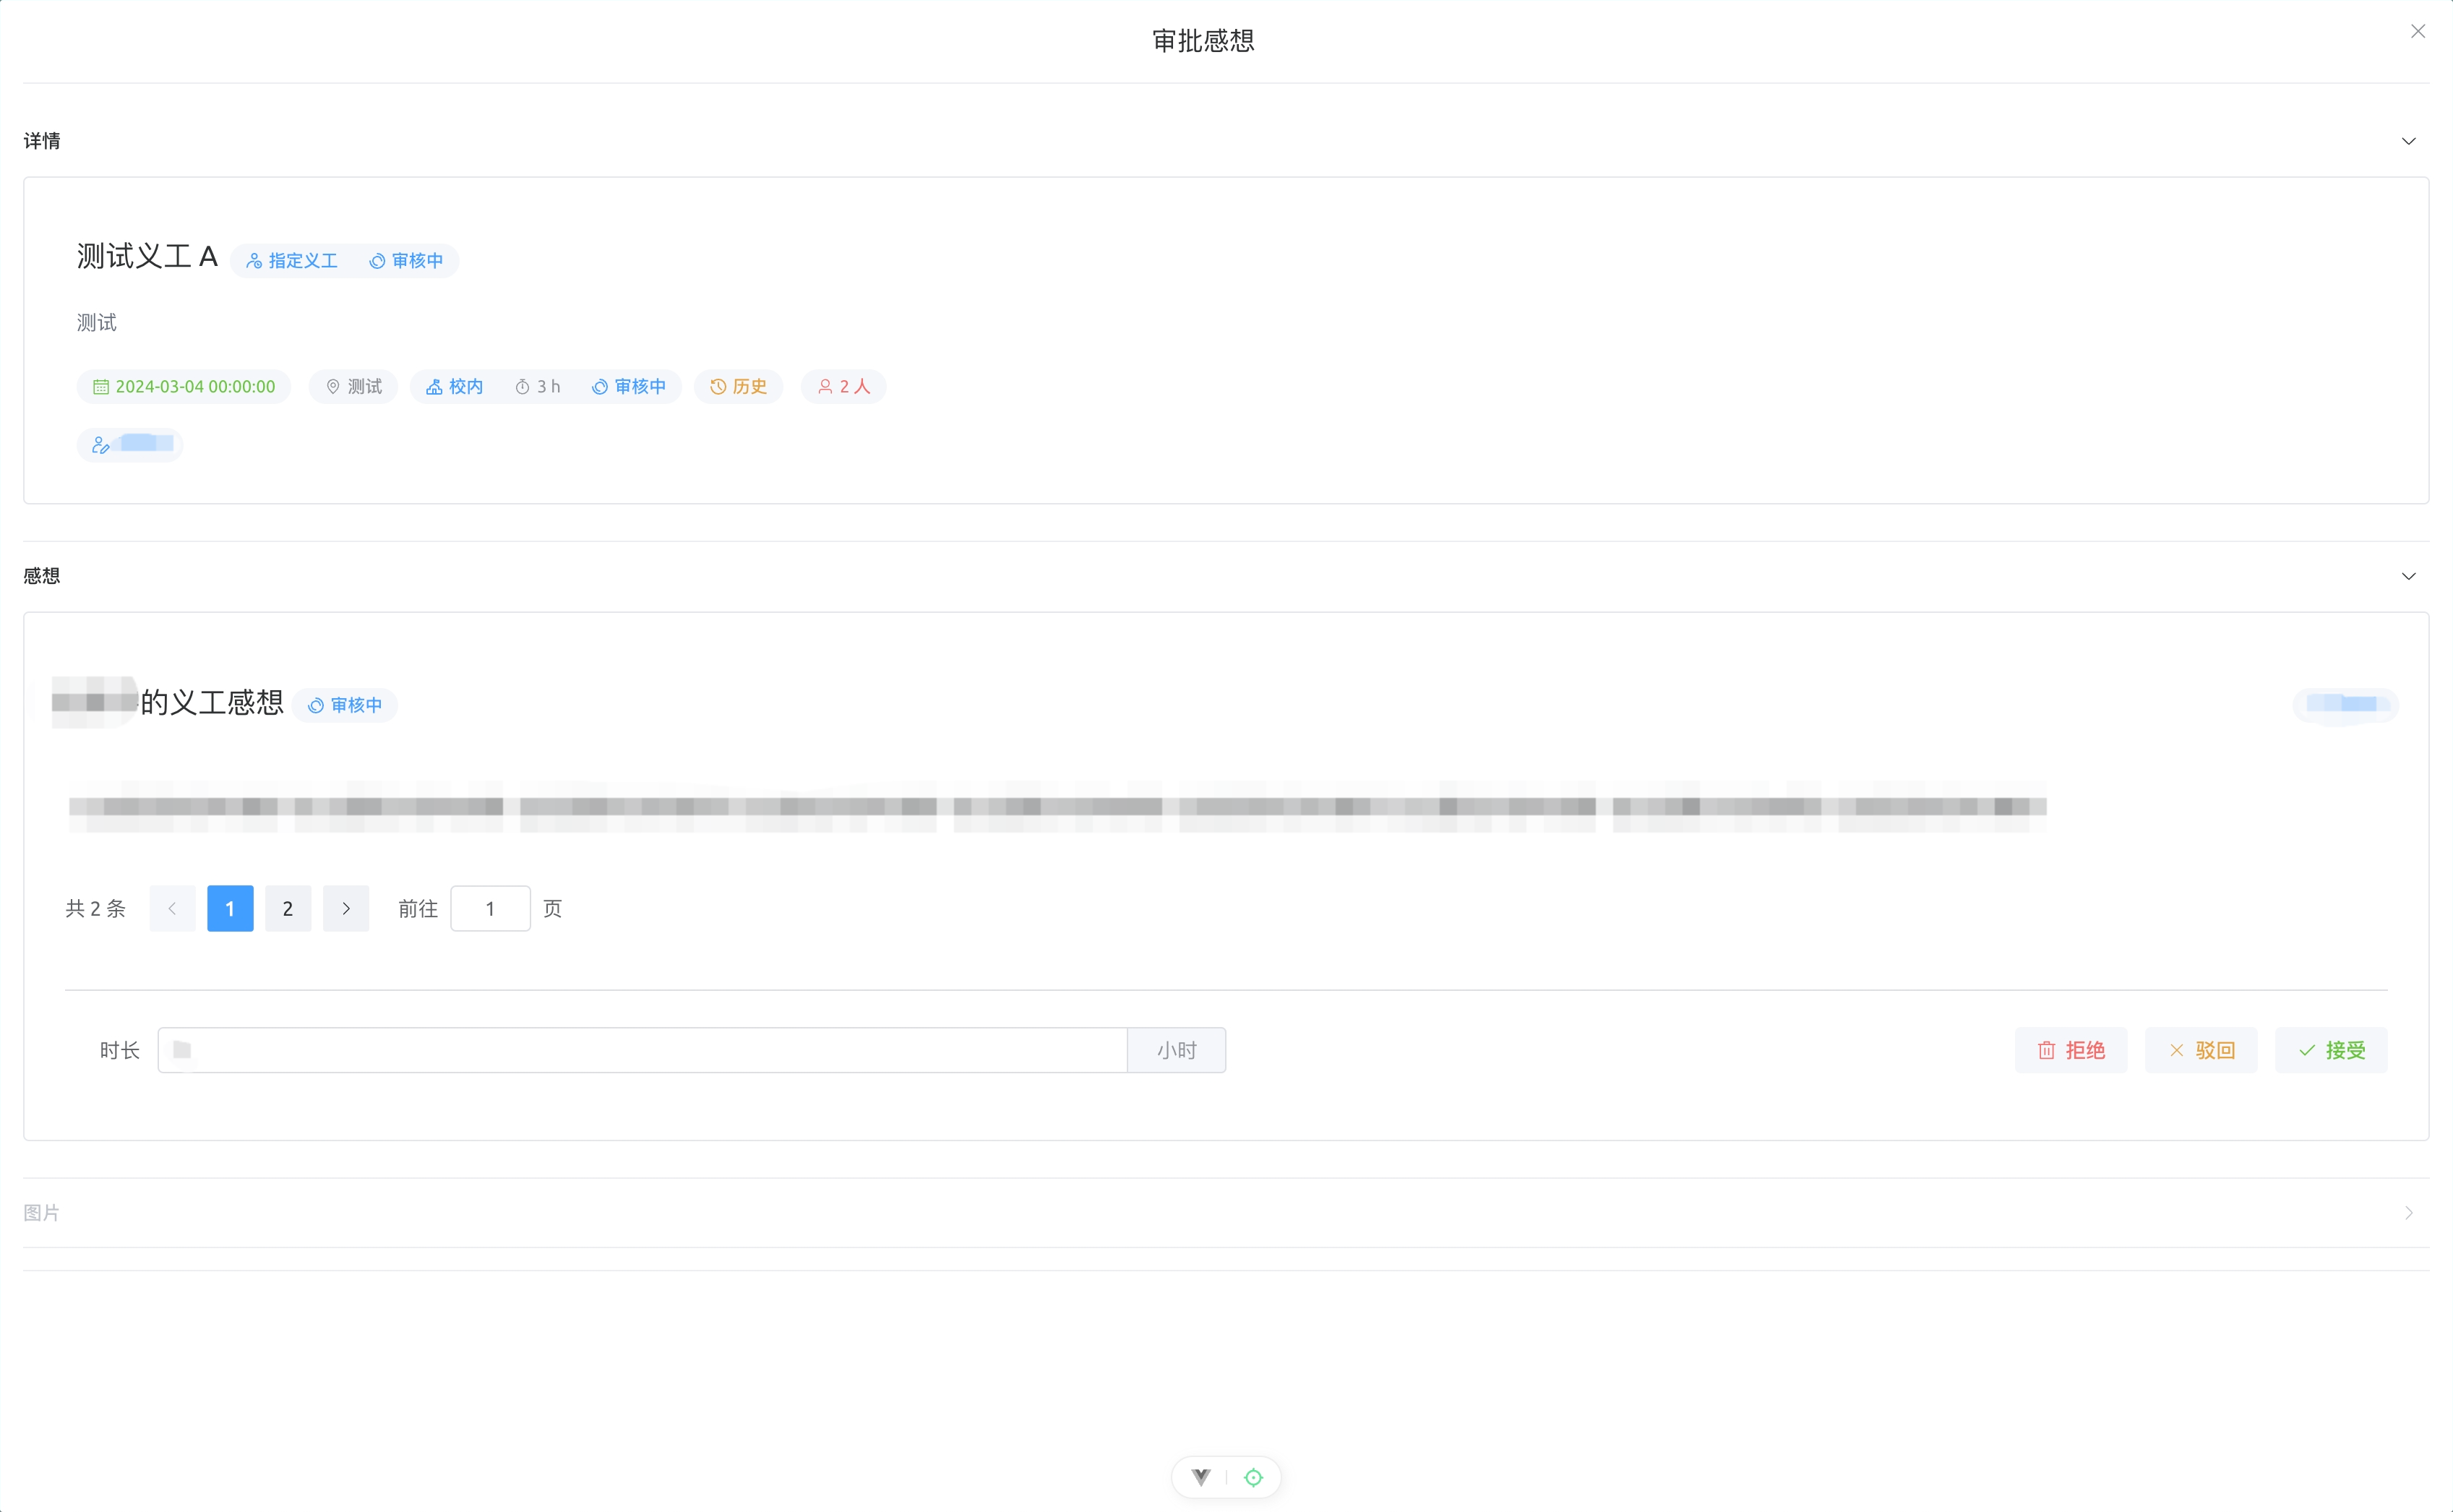
\includegraphics[width=0.8\textwidth]{../assets/image-20240303154558556.png}
  \caption{审核感想}
  \label{fig:volunteer-feelings-audit}
\end{figure}

同时, 可以根据实际情况修改原纪录的义工时长, 但不应当超过一定数值.

\begin{figure}[H]
  \centering
  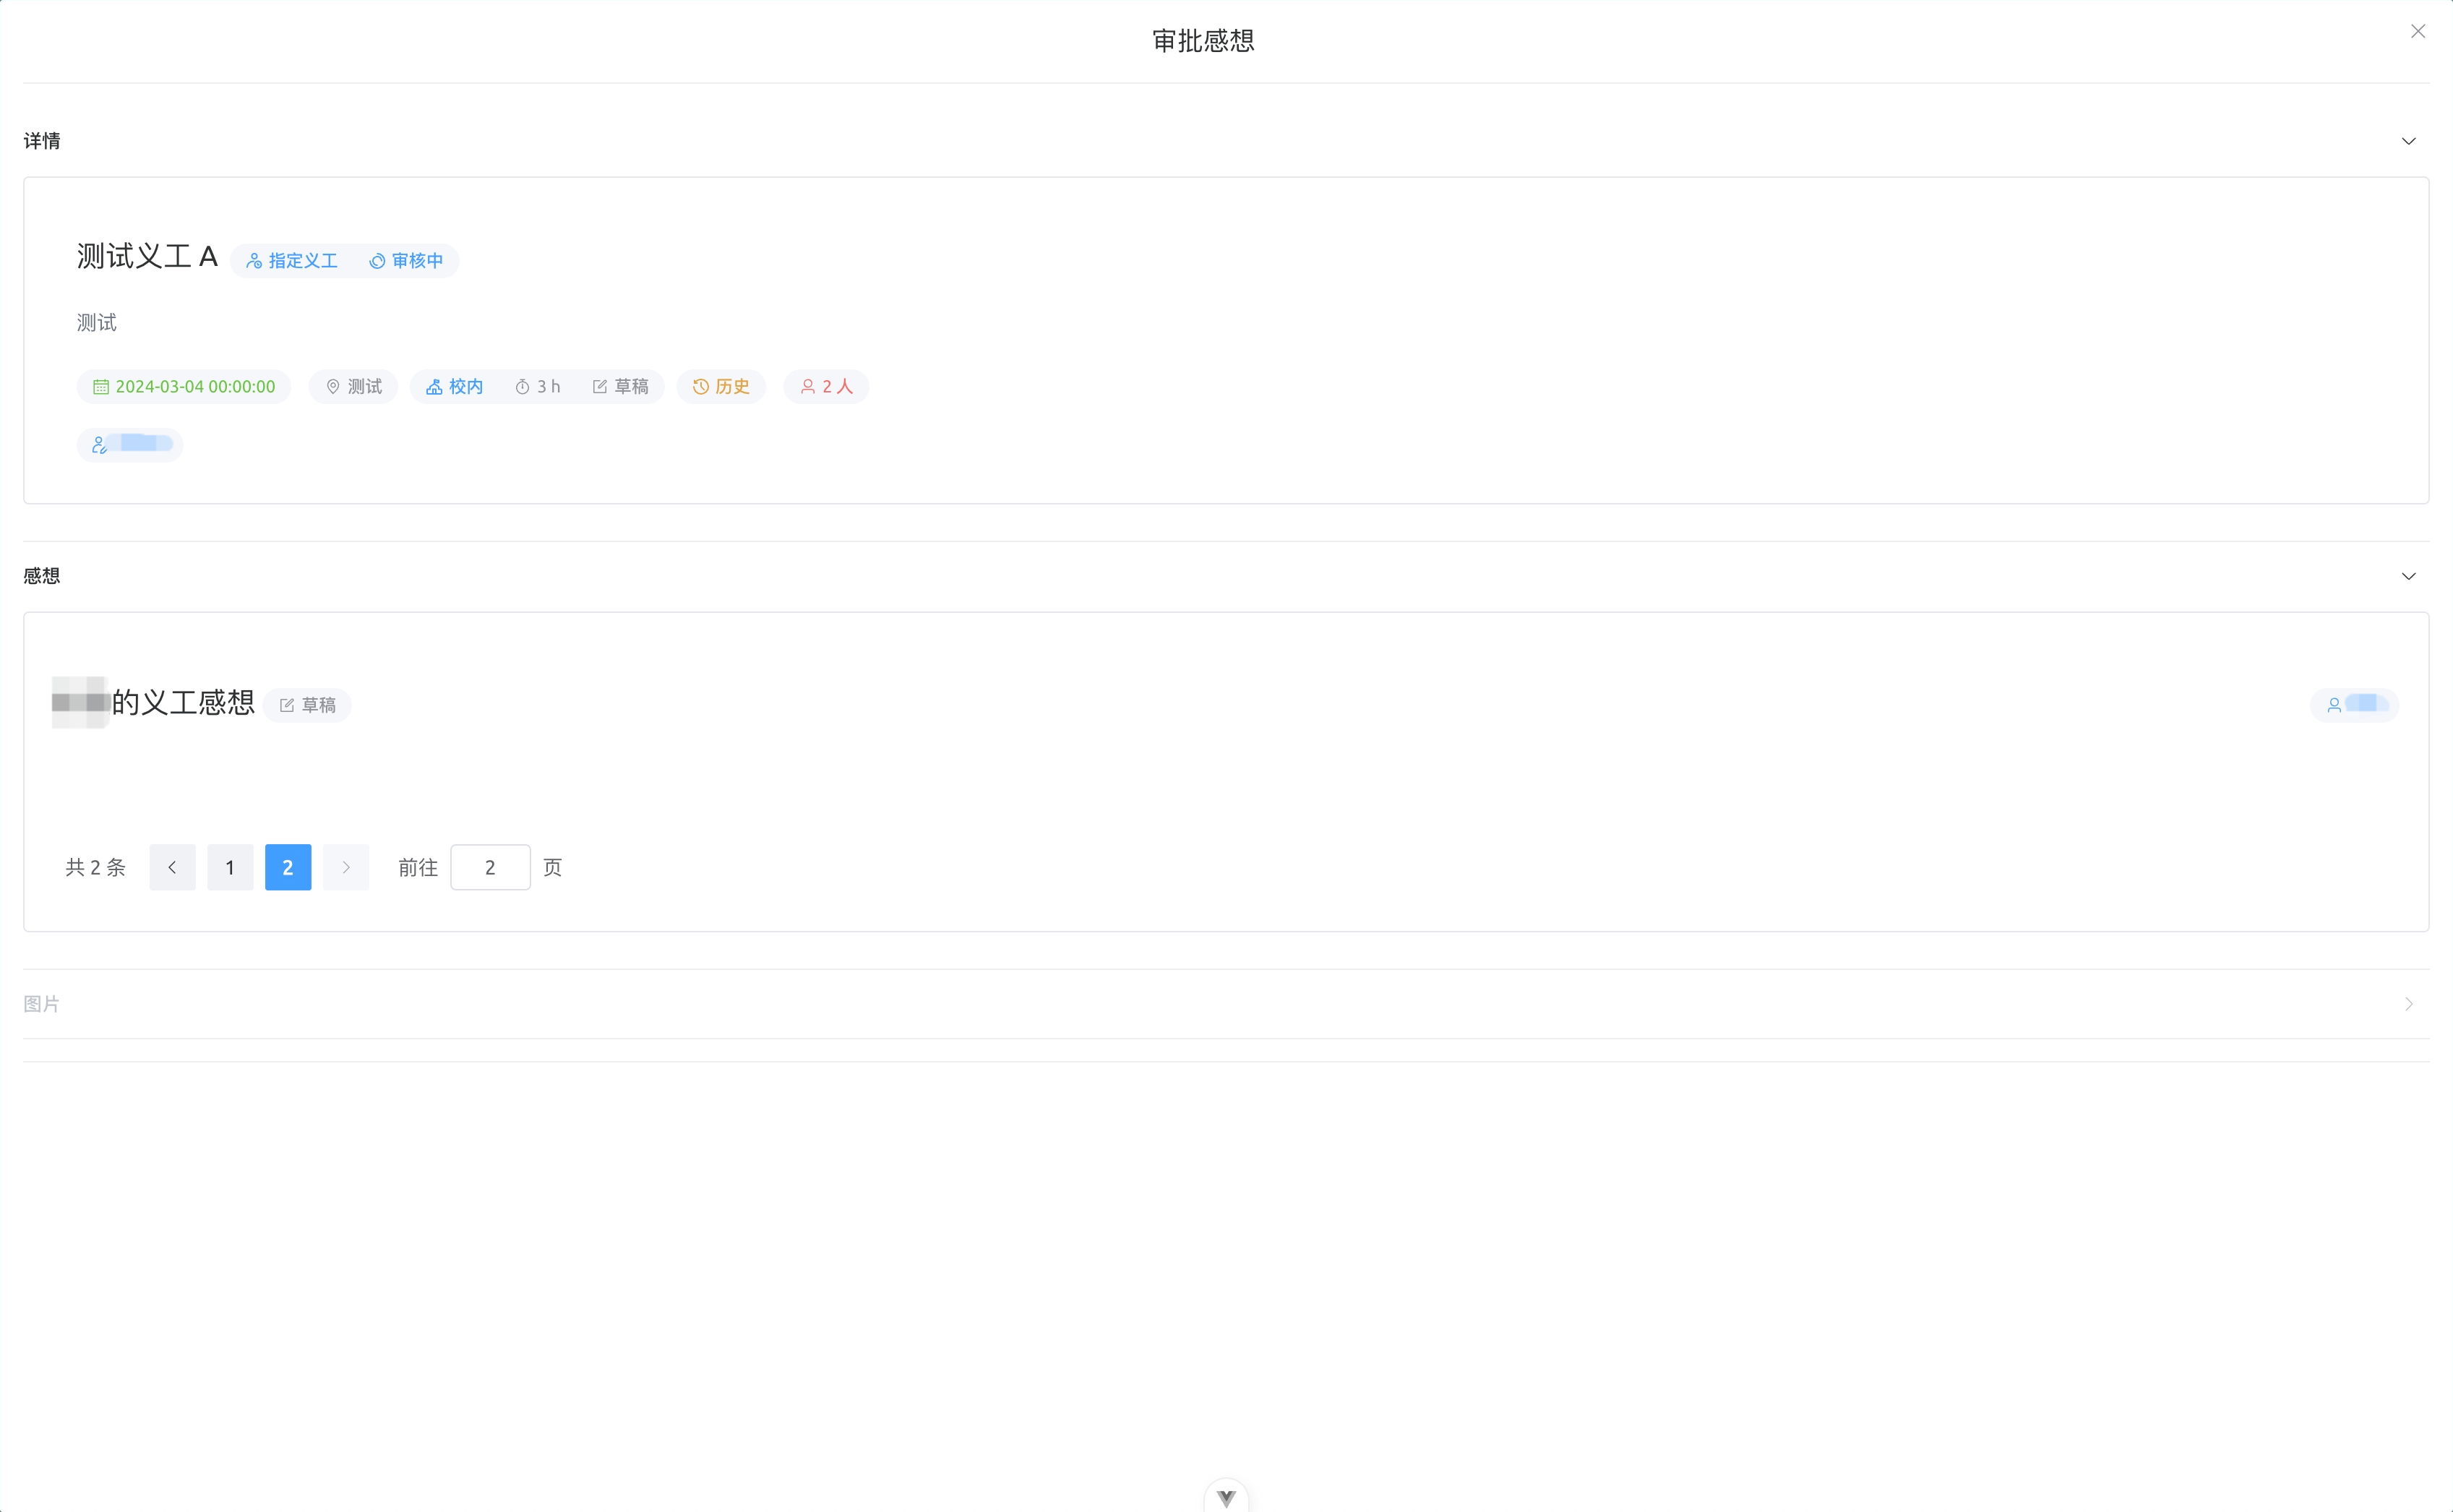
\includegraphics[width=0.8\textwidth]{../assets/image-20240303161514901.png}
  \caption{审核感想}
  \label{fig:volunteer-feelings-audit-time}
\end{figure}

点击相关按钮后, 将会自动跳转到下一条. 当最后一条完成审核后, 将会自动关闭窗口并刷新. 状态调整为 ``有效'' 后, 义工时间才会发放.

\begin{figure}[H]
  \centering
  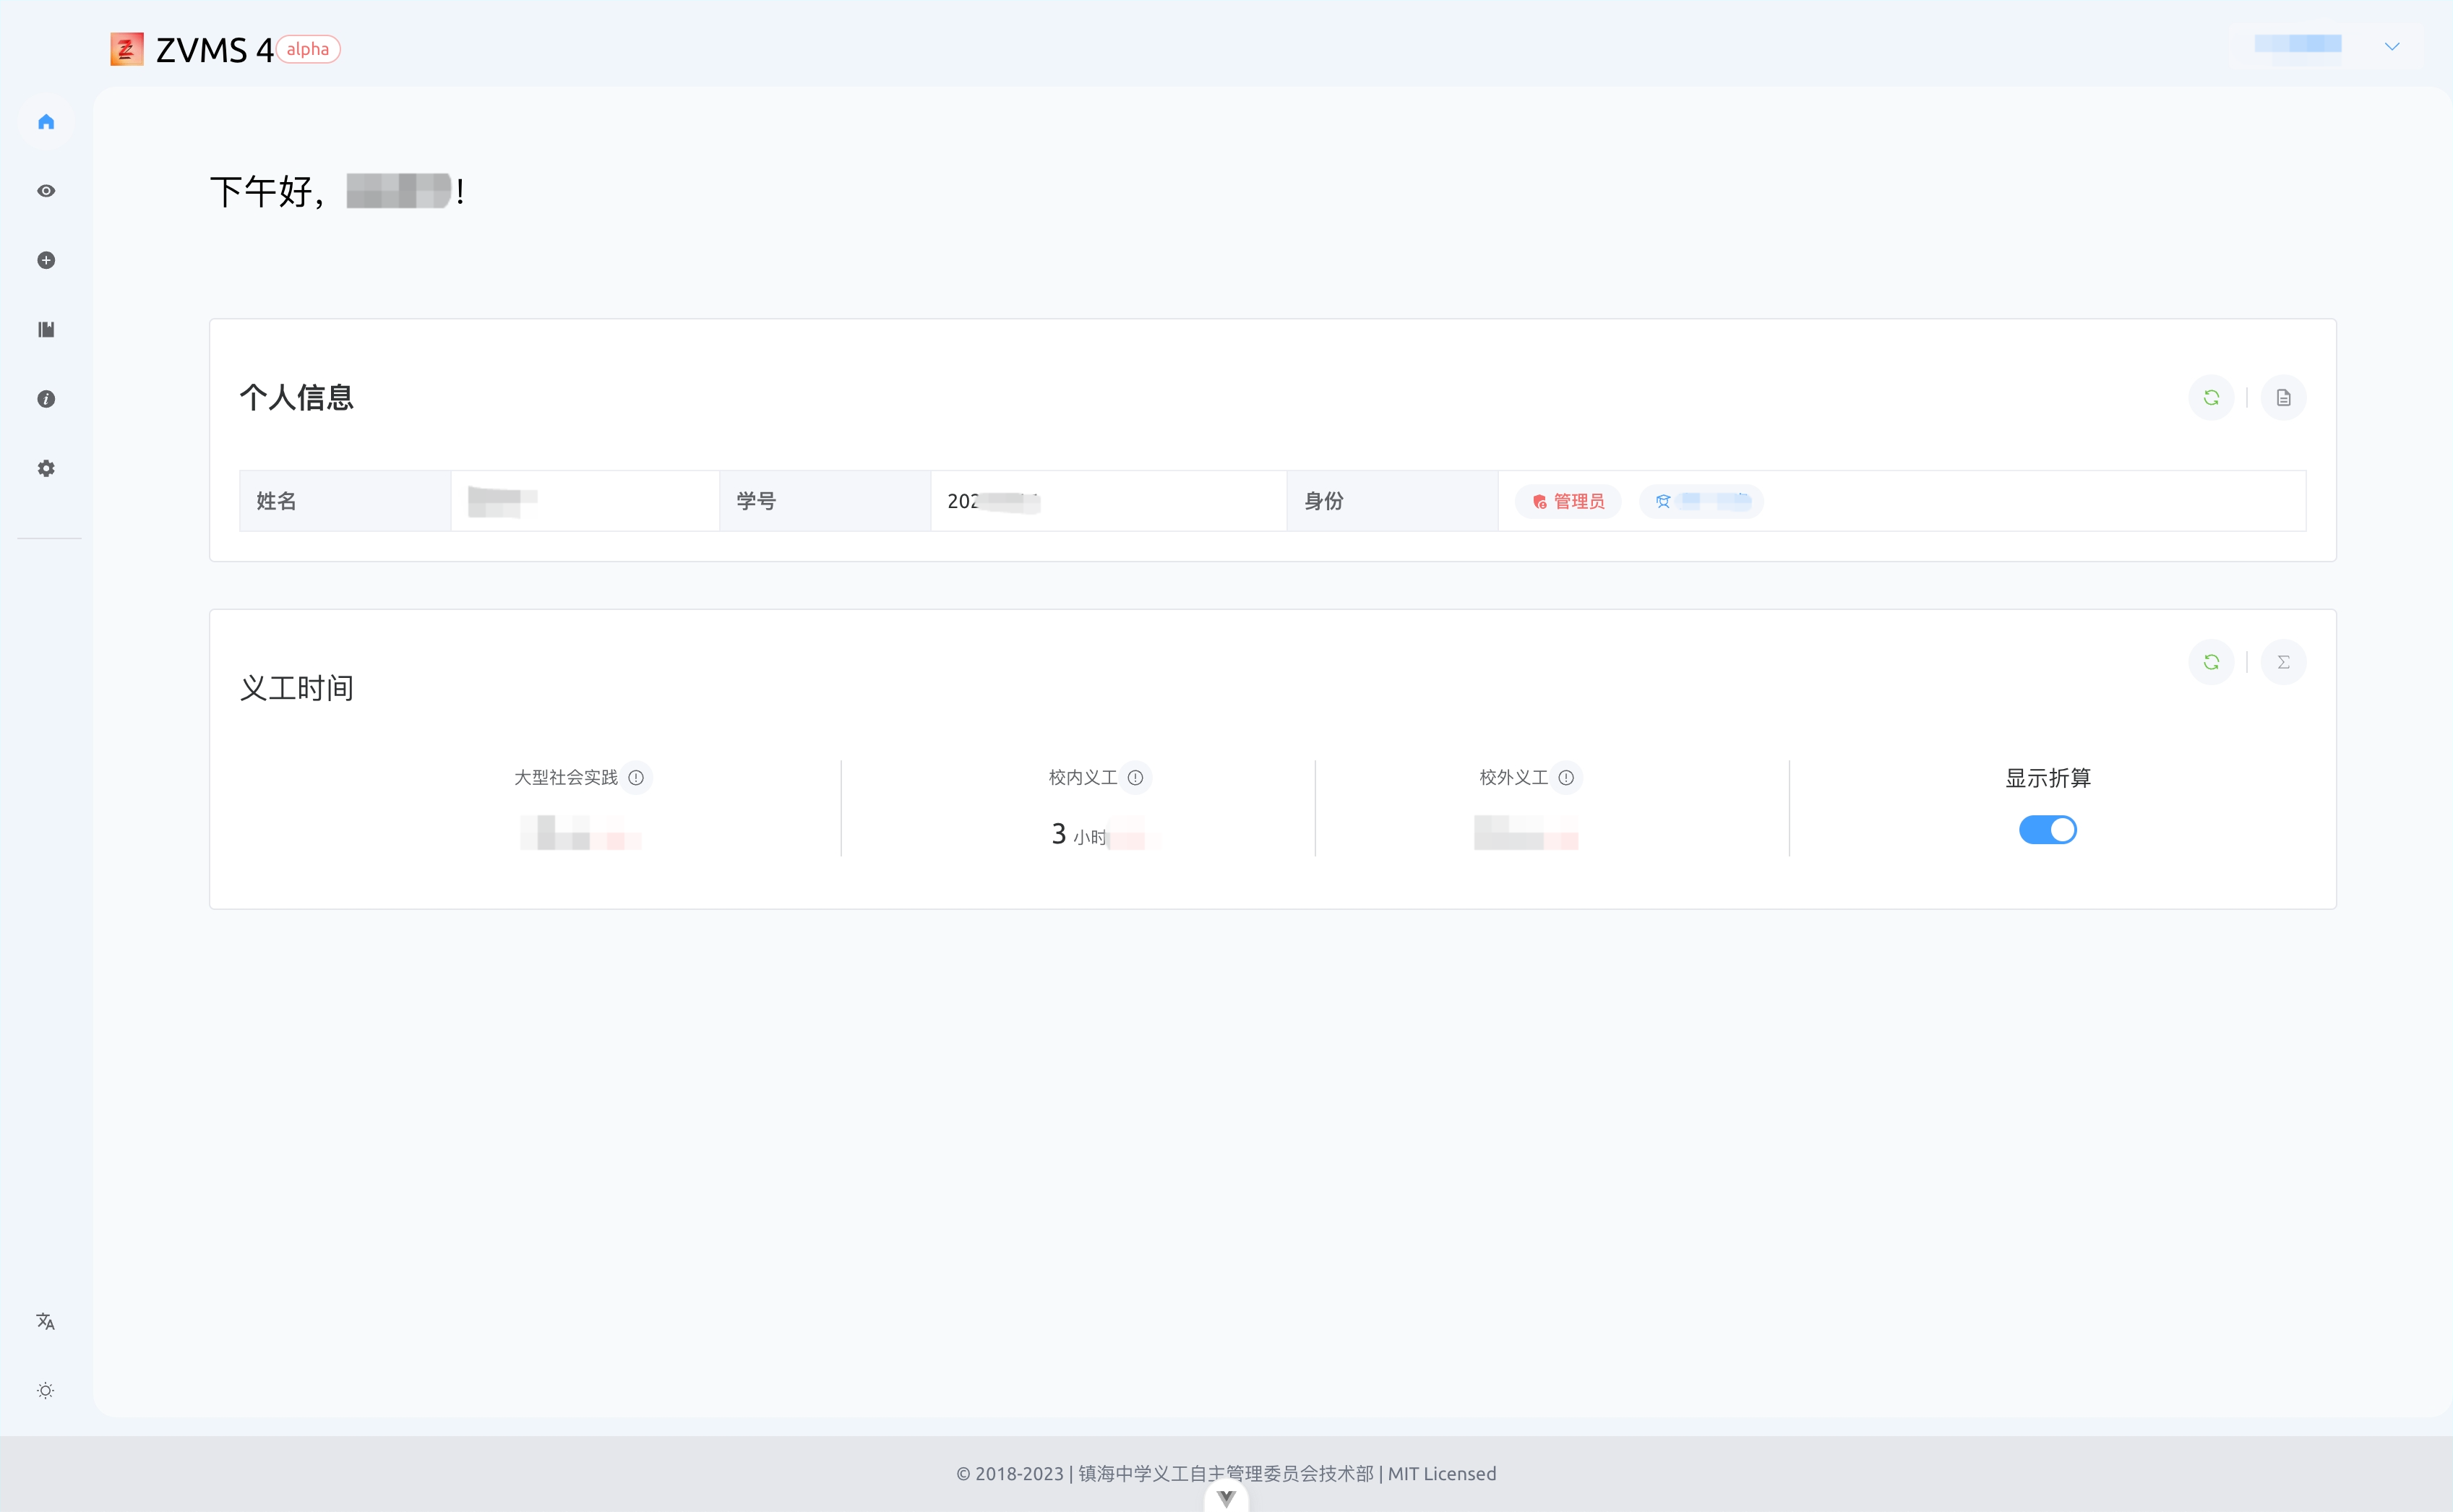
\includegraphics[width=0.8\textwidth]{../assets/image-20240303161949915.png}
  \caption{审核感想}
  \label{fig:volunteer-feelings-audit-finish}
\end{figure}

\subsection{成员管理}

在详细卡片界面, 您可以点击 ``成员'' ($n$ 人) 打开成员管理页面.

\begin{figure}[H]
  \centering
  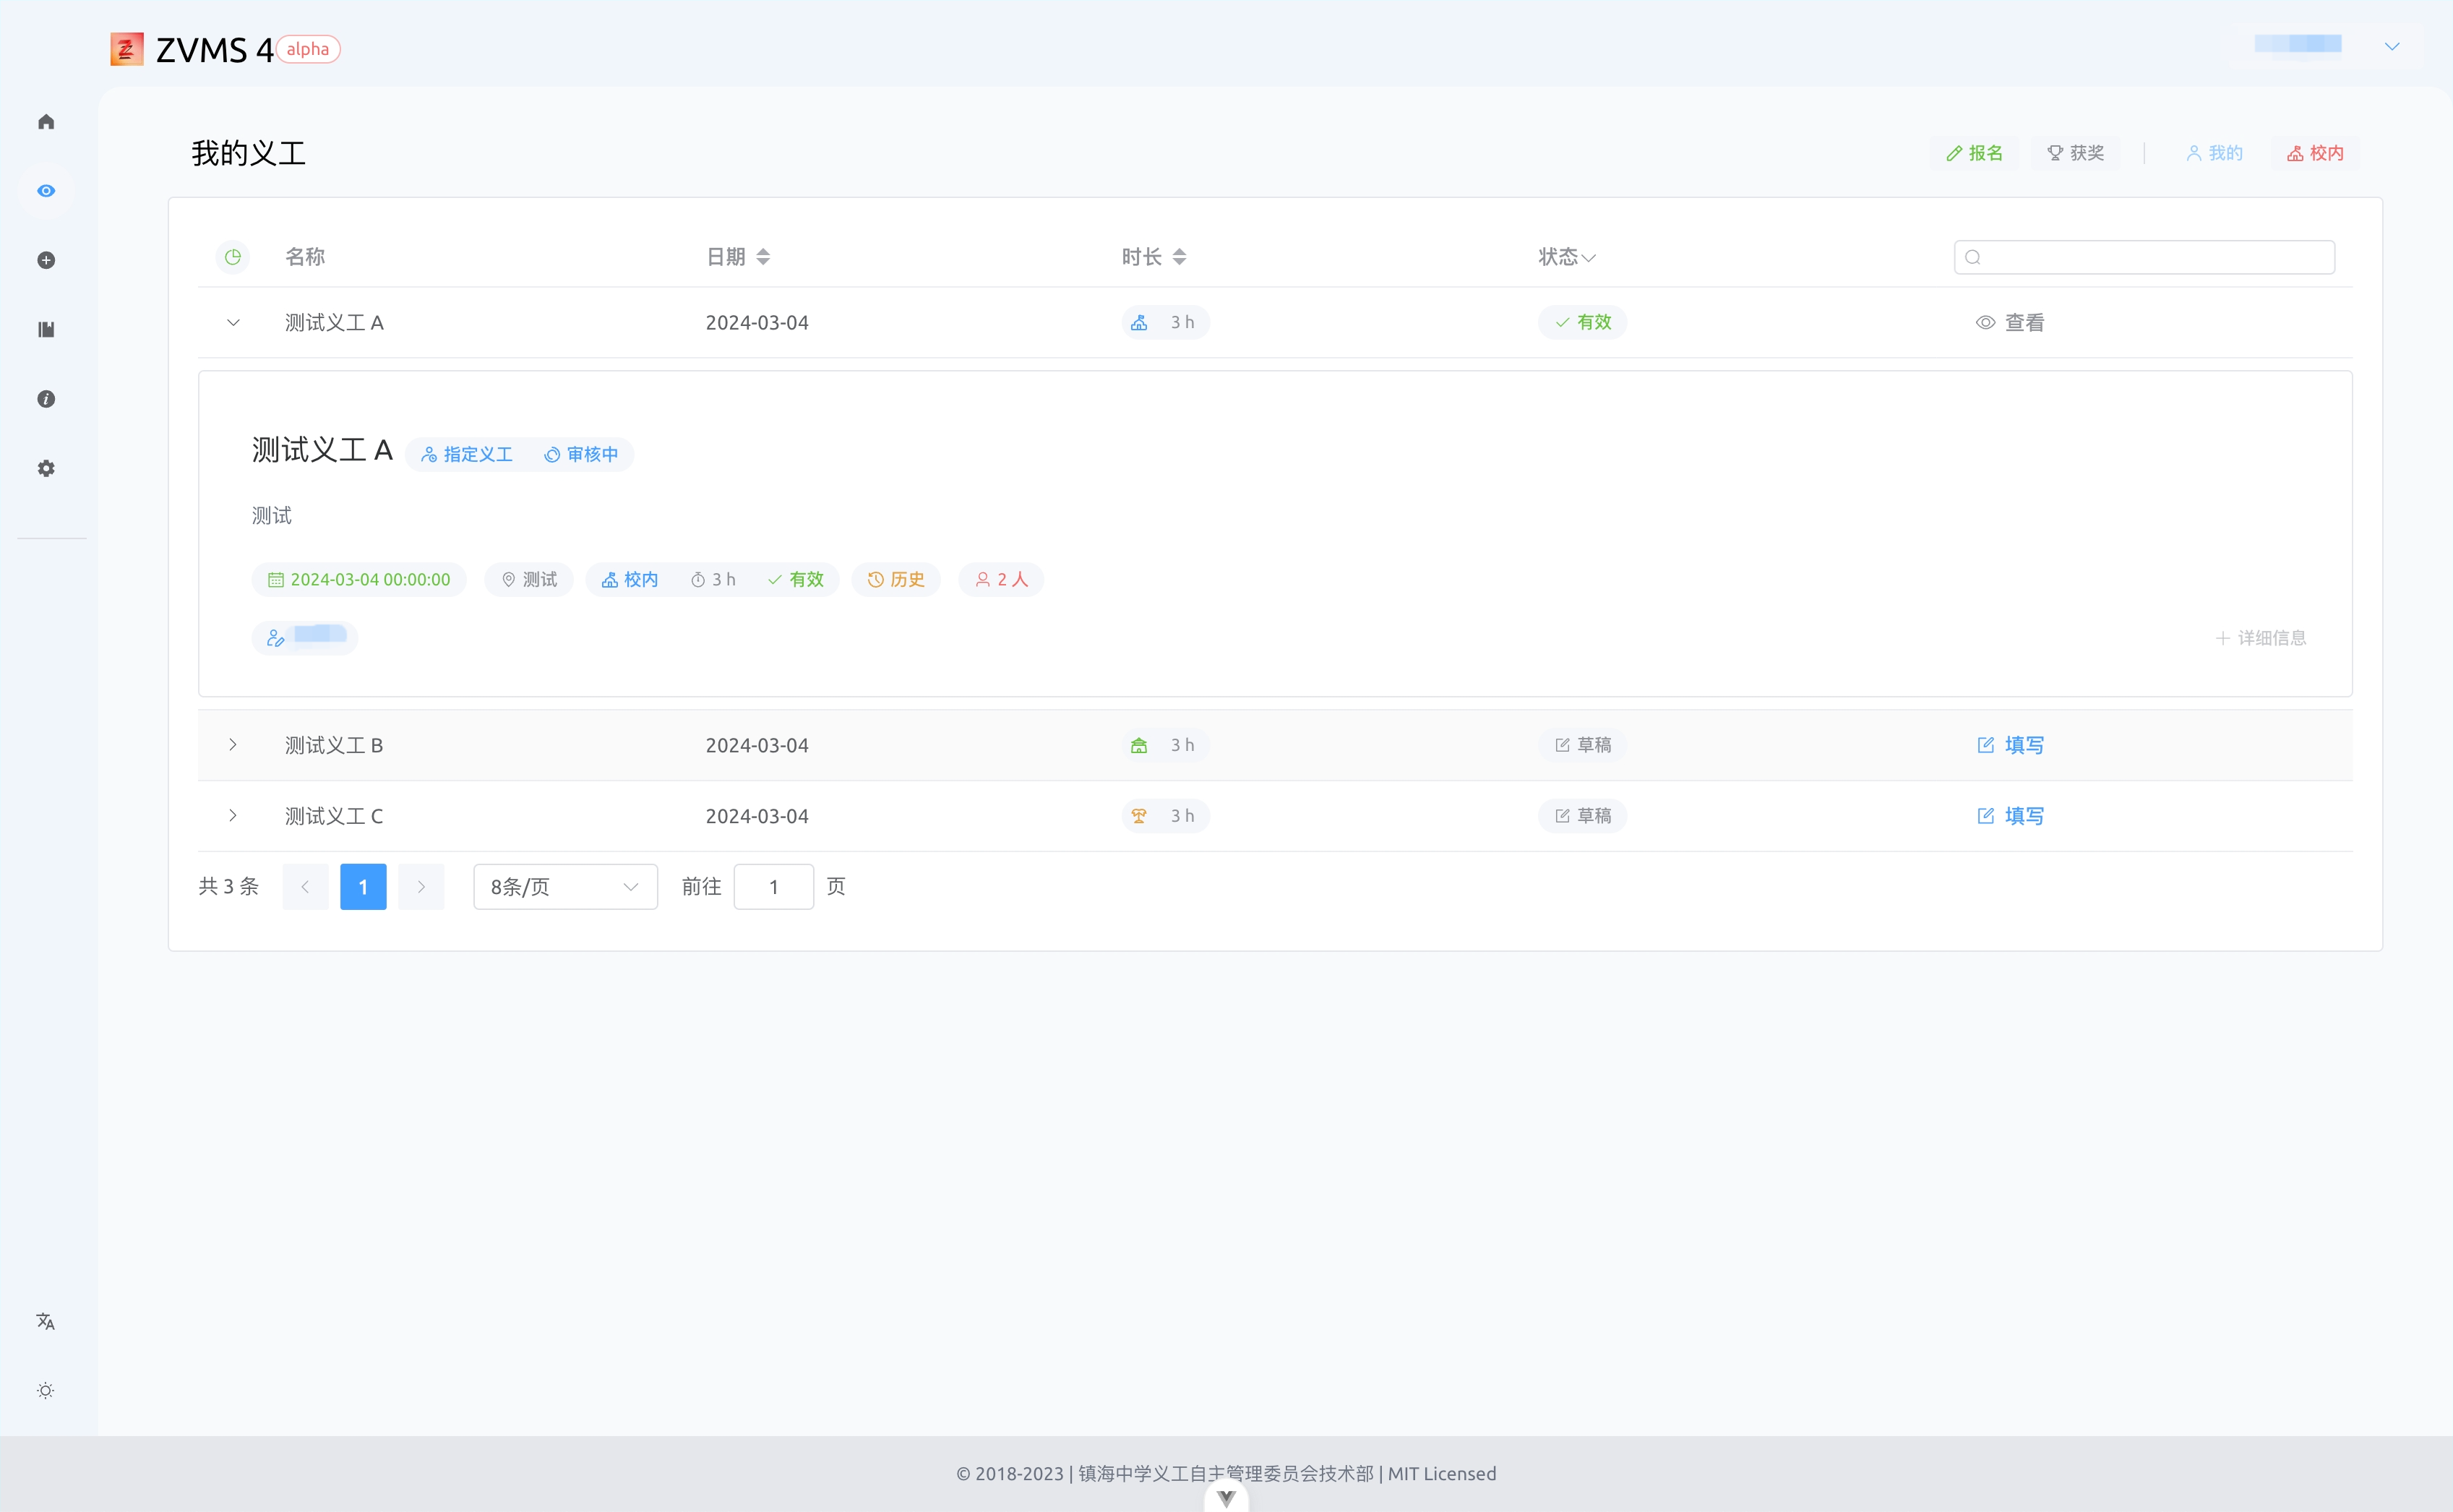
\includegraphics[width=0.8\textwidth]{../assets/image-20240303164247303.png}
  \caption{成员管理}
  \label{fig:volunteer-member}
\end{figure}

点击后, 将会打开对话框. 您可以在这里添加或删除成员.

\begin{figure}[H]
  \centering
  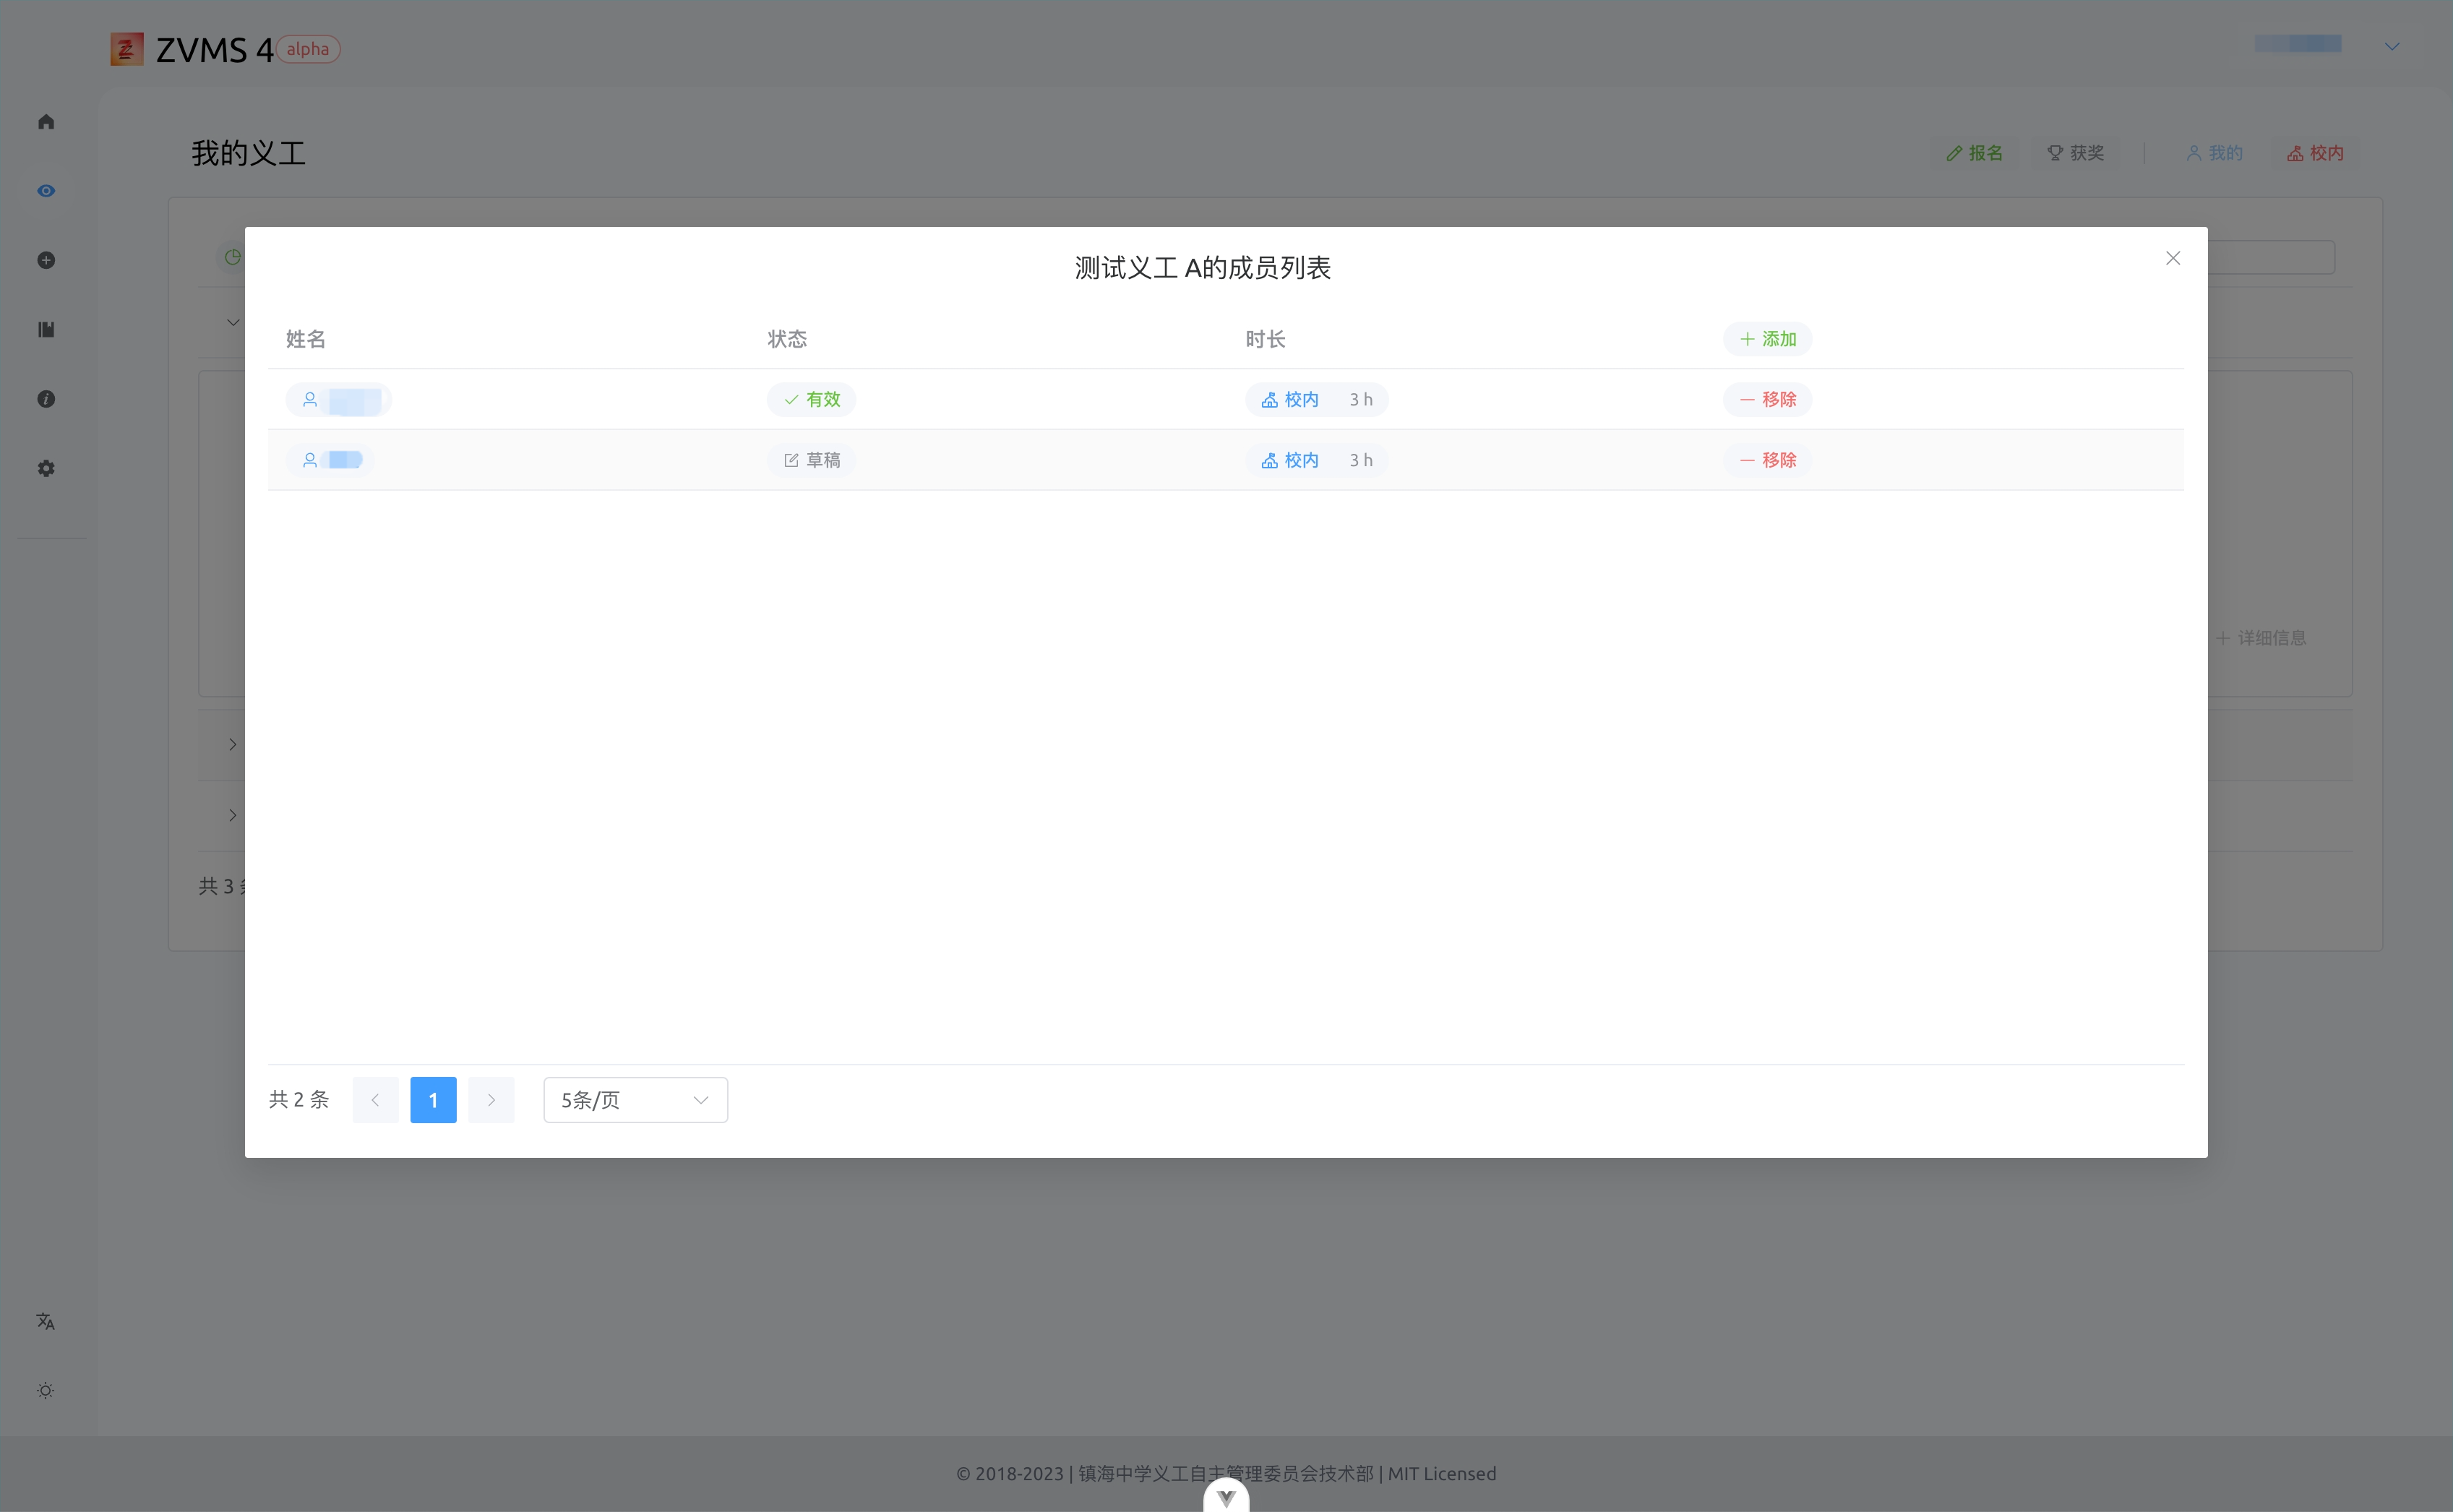
\includegraphics[width=0.8\textwidth]{../assets/image-20240303164326424.png}
  \caption{成员管理}
  \label{fig:volunteer-member-dialog}
\end{figure}

值得注意的是, 团支书只能添加 (或删除) 本班同学 (且义工必须为非特殊义工). 个人账号无法添加或删除, 也无法退出某项义工.

\begin{figure}[H]
  \centering
  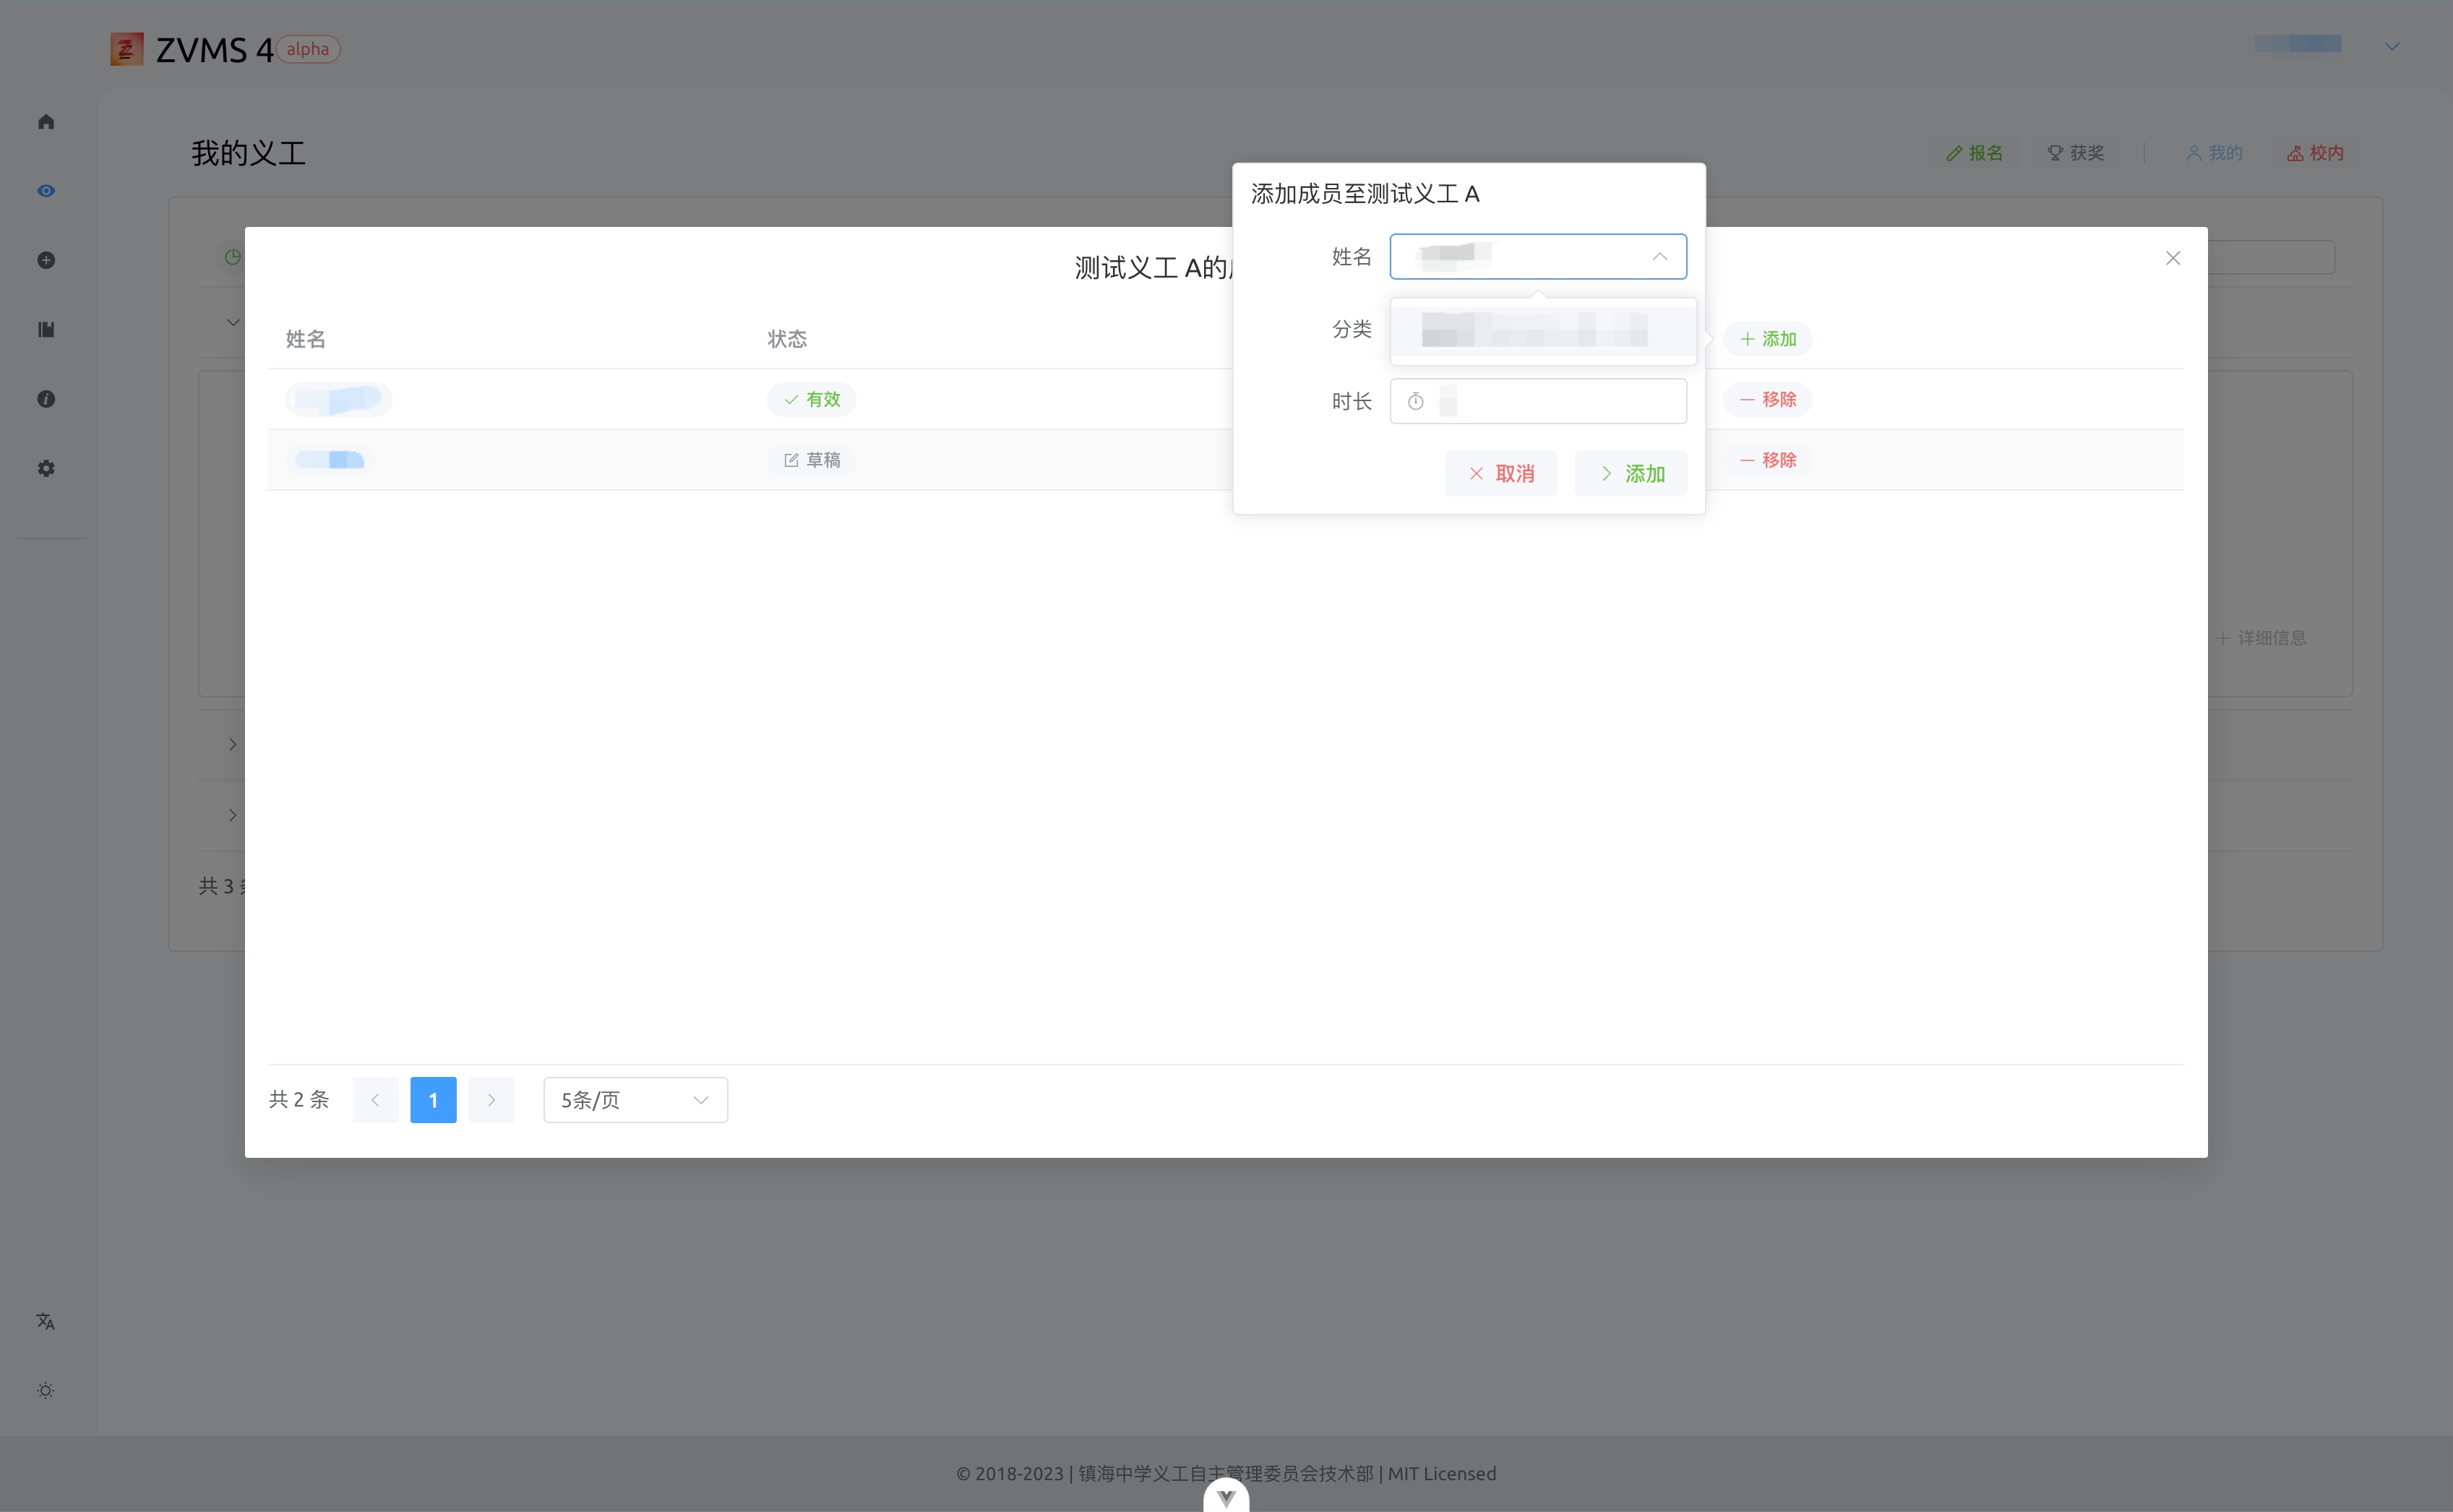
\includegraphics[width=0.8\textwidth]{../assets/image-20240303164501549.png}
  \caption{成员管理}
  \label{fig:volunteer-member-dialog-error}
\end{figure}

\section{获奖页面}

从 V4 开始, 使用 \texttt{Trophy} 页面统一填报获奖义工.

\subsection{填报获奖}

\begin{mdframed}
  \fangsong
  请注意, 在中文版中, \texttt{Trophy} 和 \texttt{Award} 都由 \texttt{GitHub Copilot} 翻译为了 ``奖项''. 但是实际请注意区分, 若无法区分请切换至英文版.
\end{mdframed}

点击 ``获奖'', 将会跳转到获奖义工填报界面. 该界面中, 可报名和参与的奖项将会在获奖主页中显示. 您可以根据您的实际情况填报相关的奖项.

\begin{figure}[H]
  \centering
  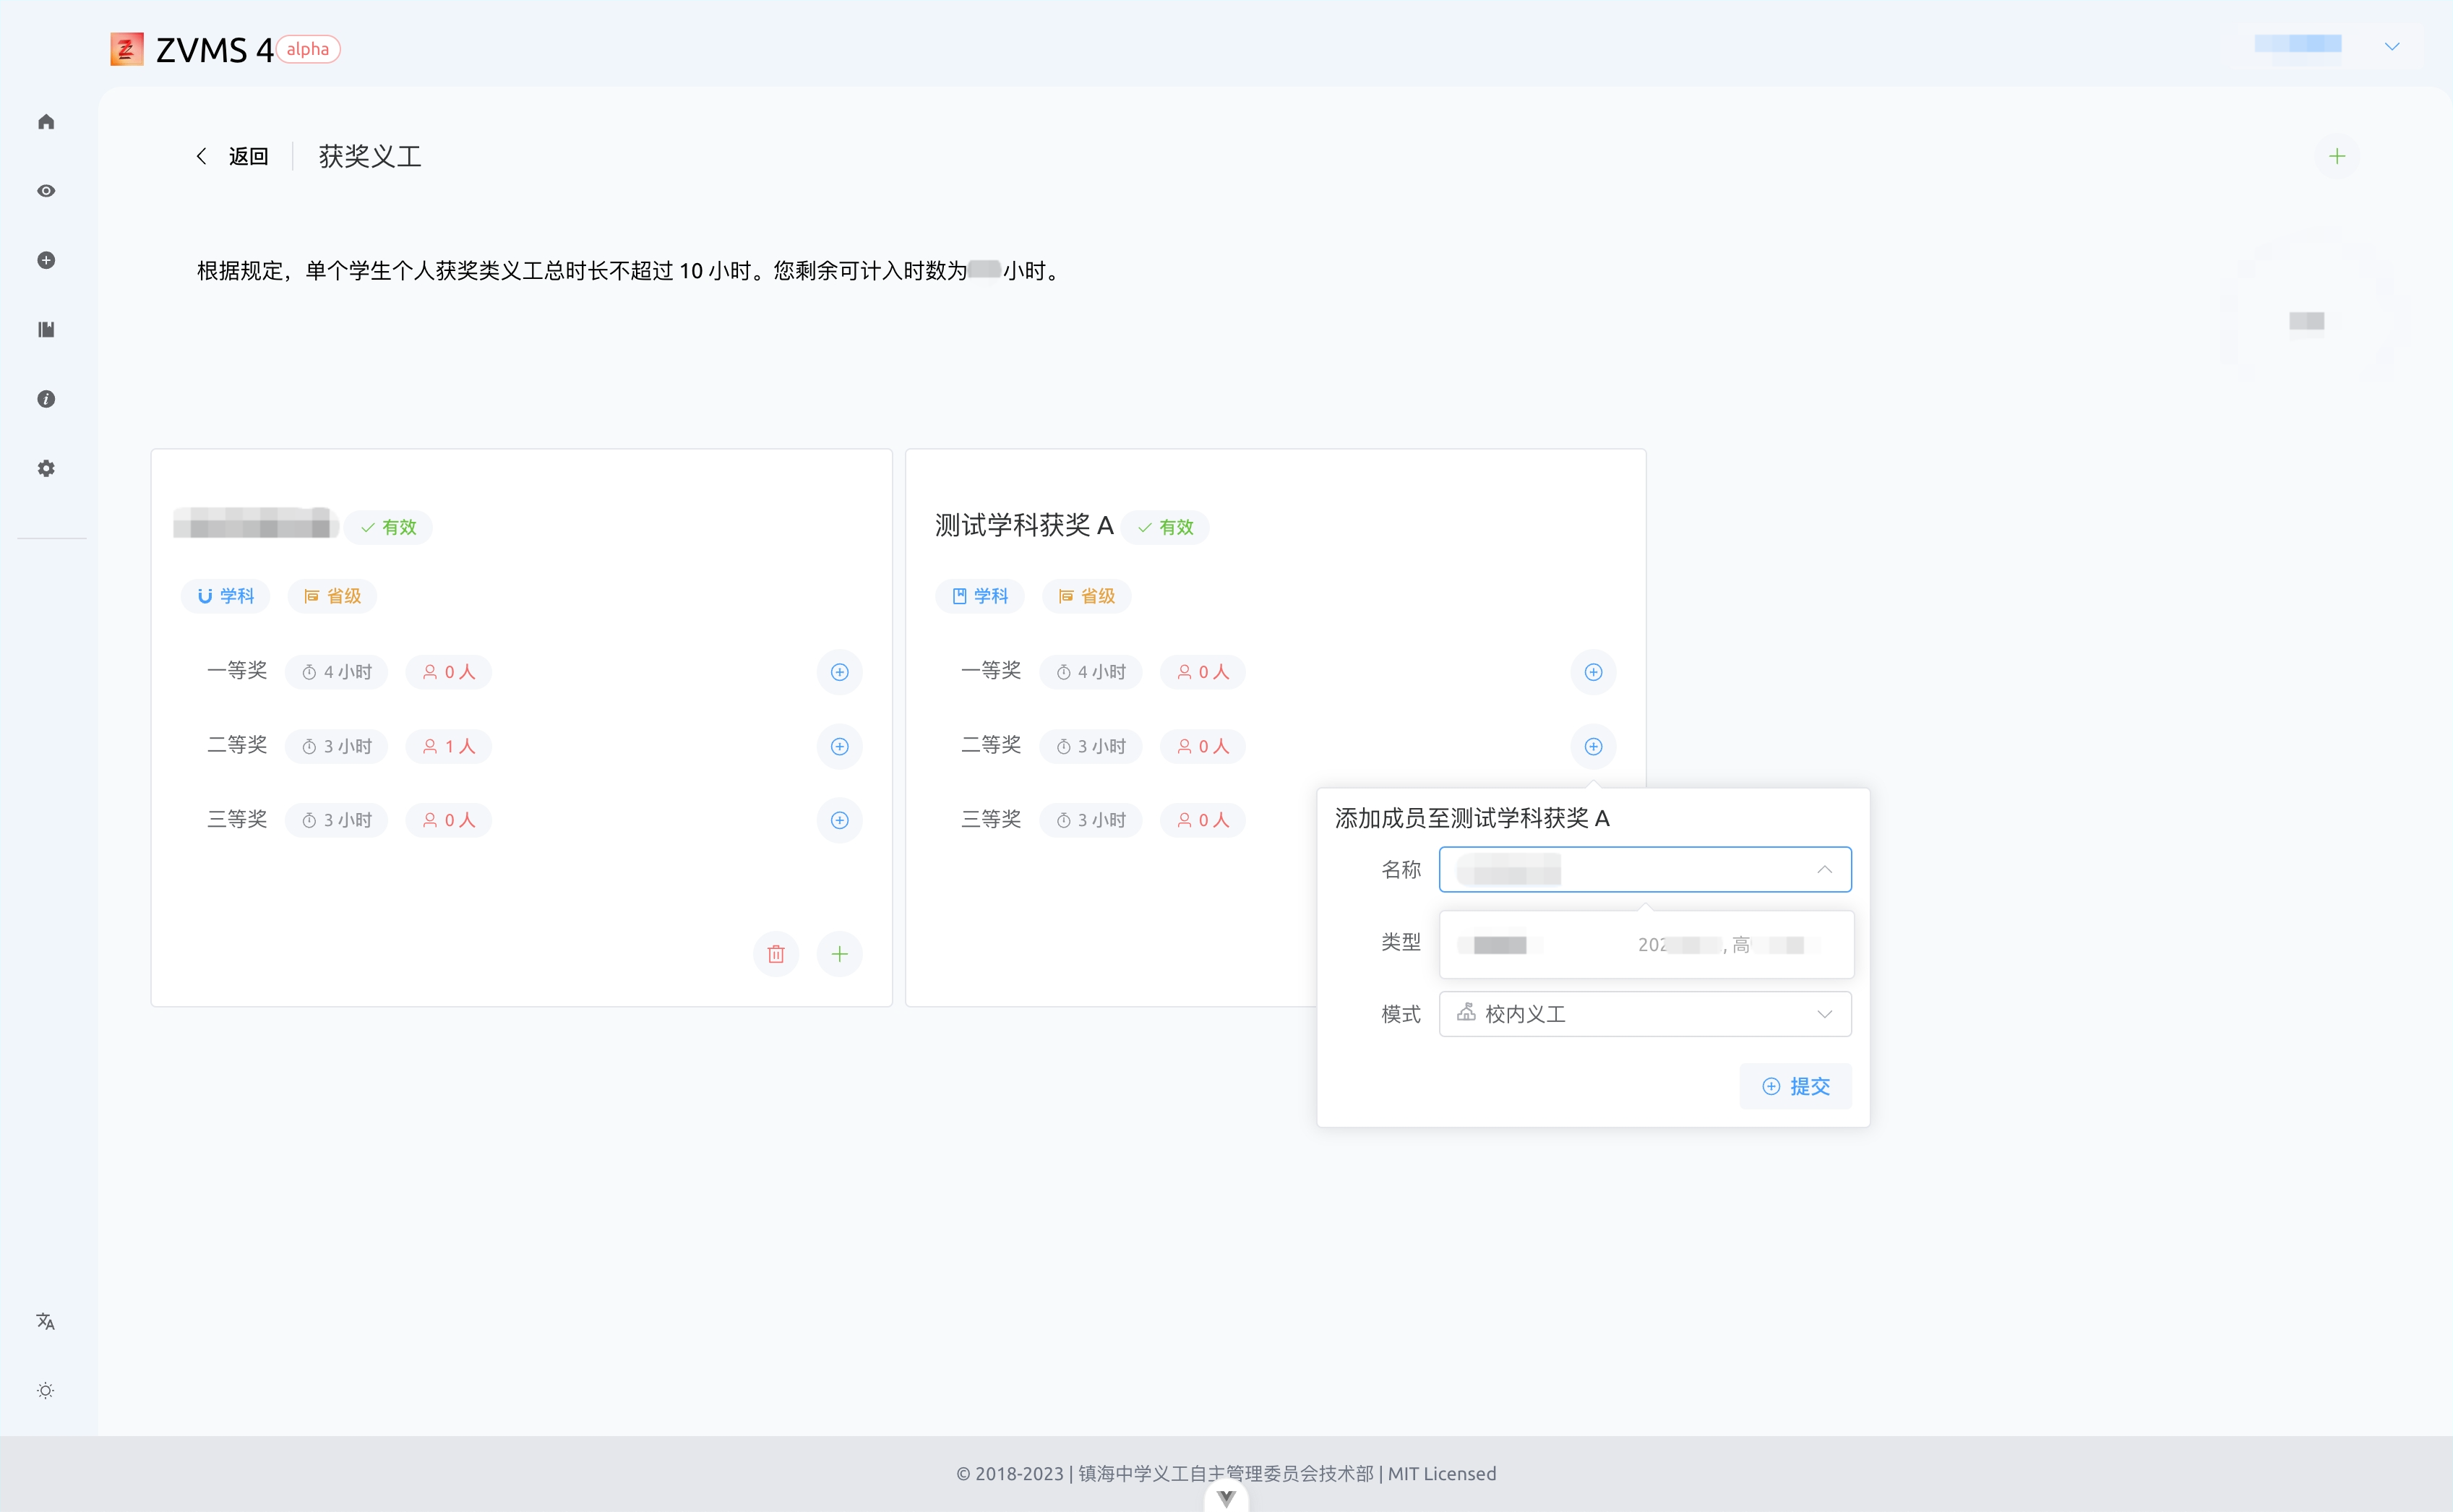
\includegraphics[width=0.8\textwidth]{../assets/image-20240303162655378.png}
  \caption{填报获奖}
  \label{fig:trophy}
\end{figure}

点击加号, 系统将自动展示您的 $\mathrm{ID}$ 和相关类型. 您可以在 ``模式'' 中自主选择记入校内或校外义工, 无需他人修改.

\begin{figure}[H]
  \centering
  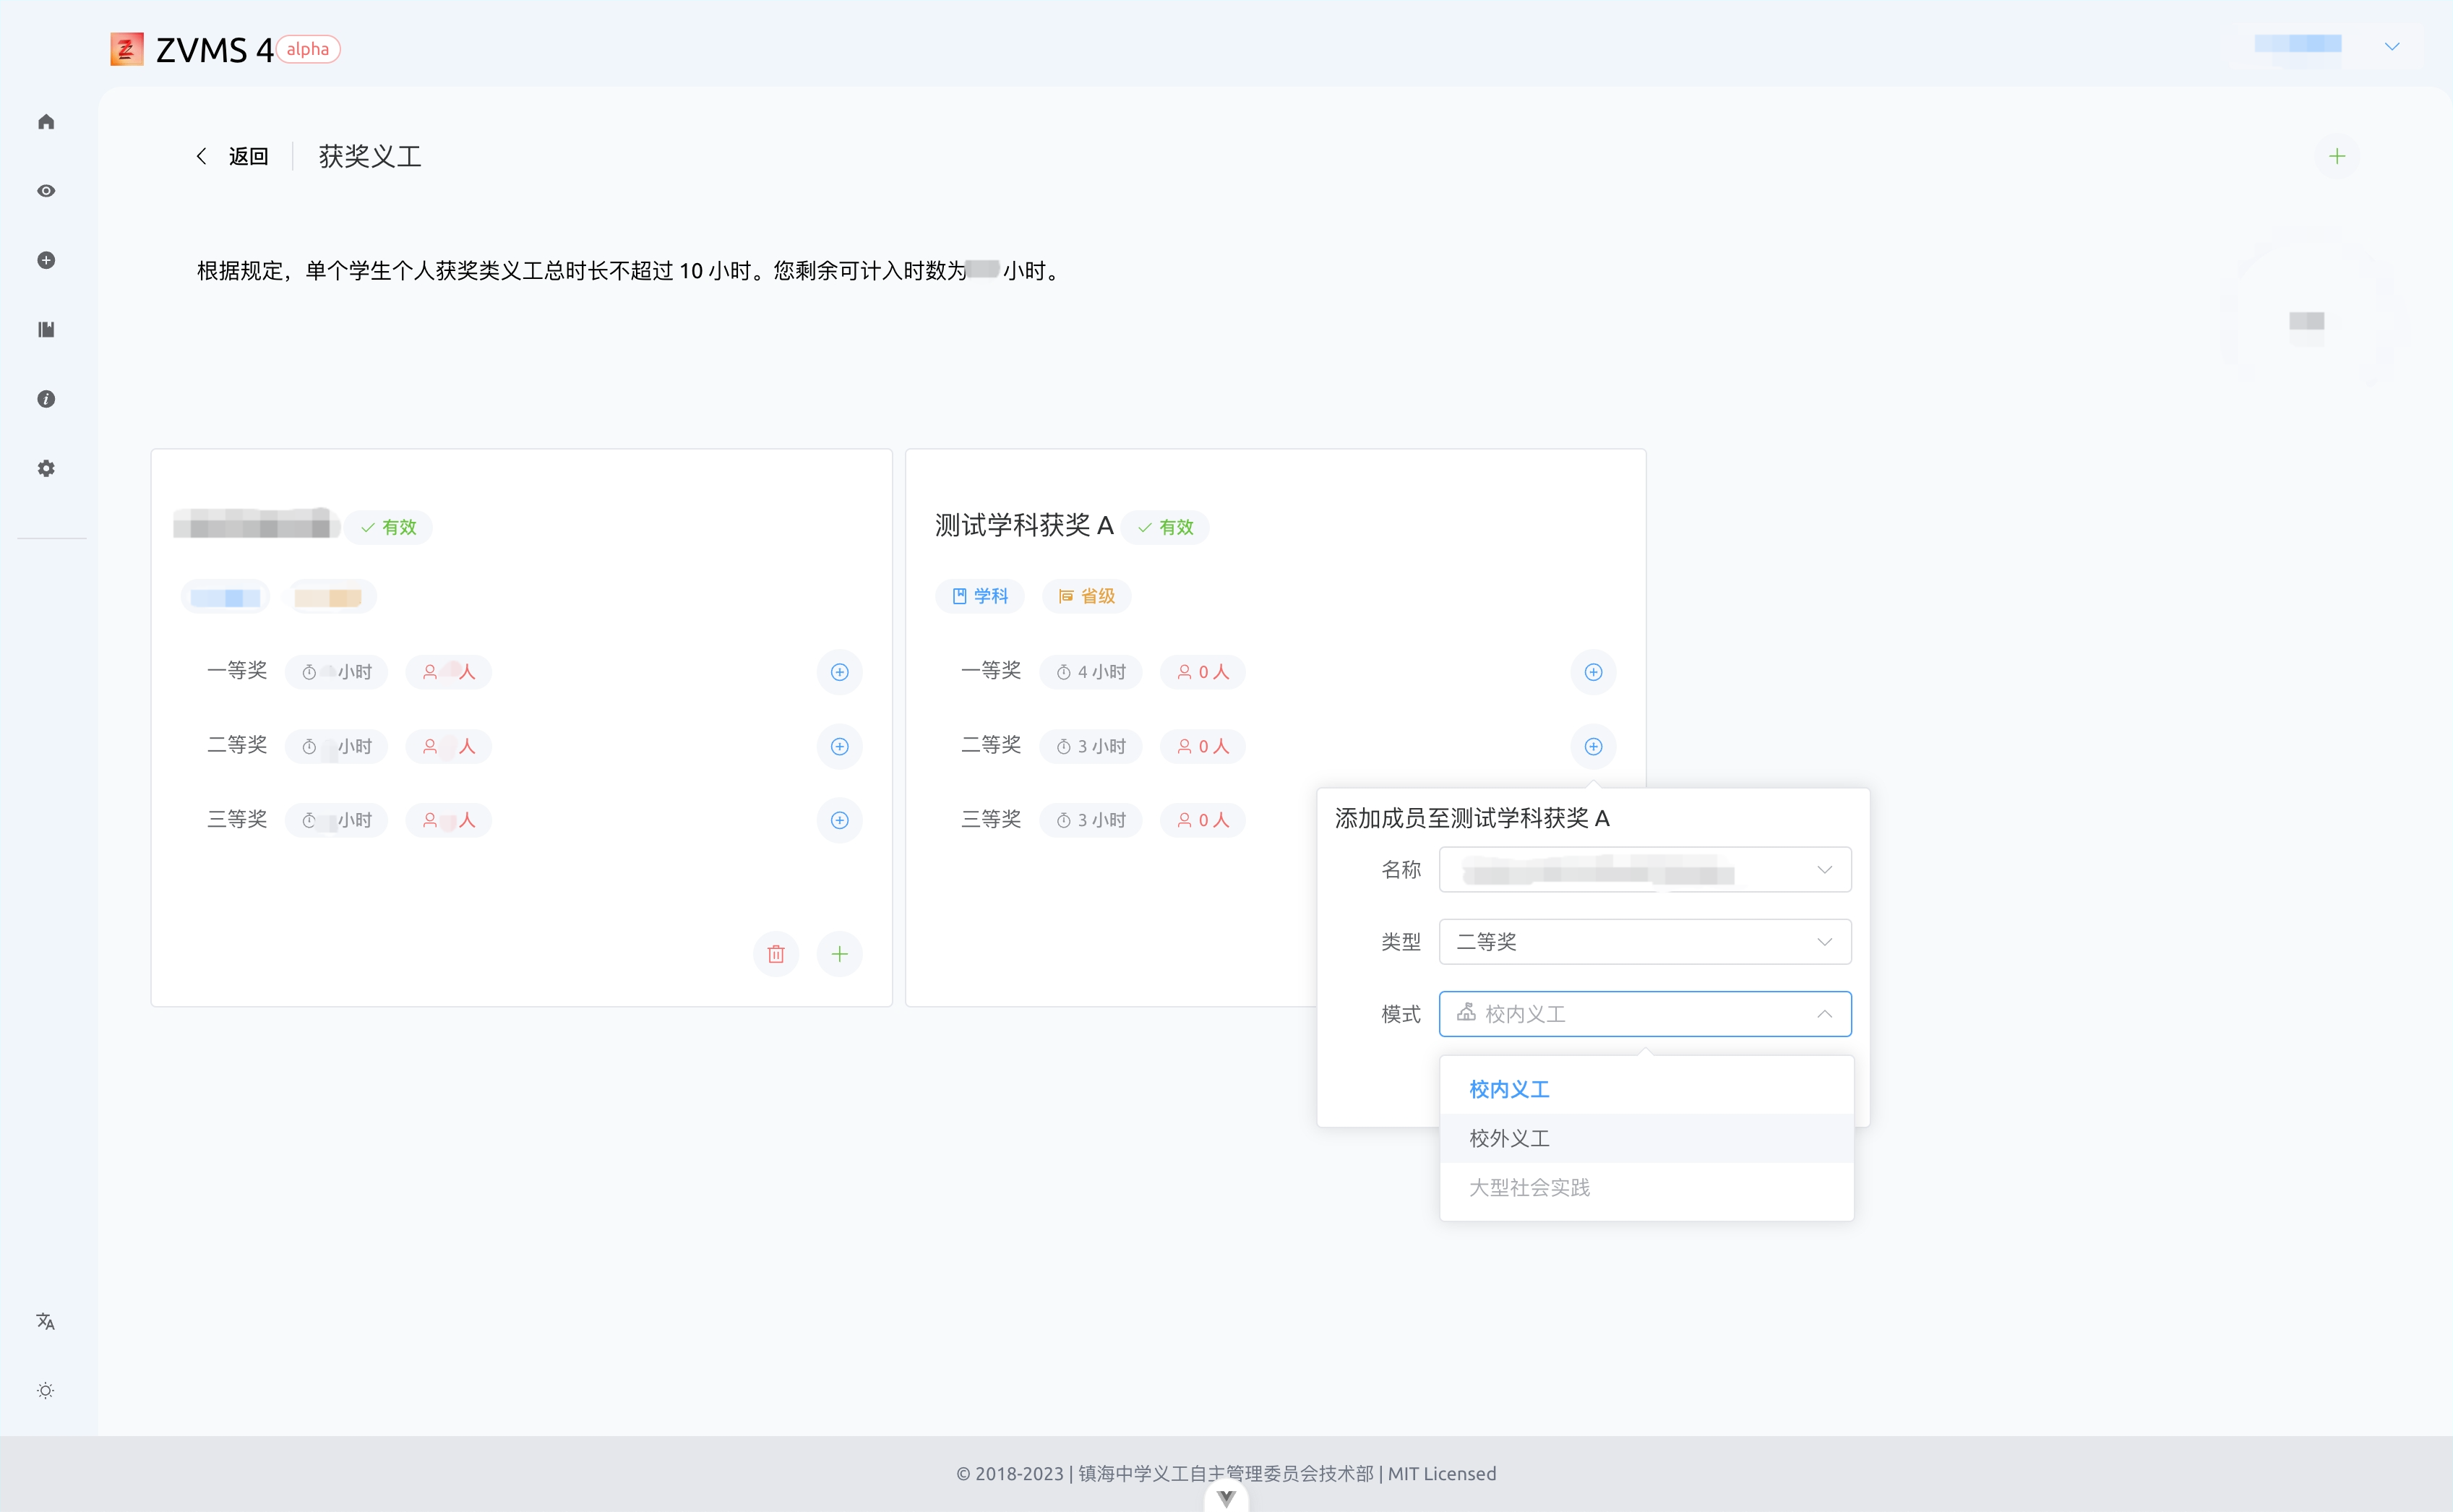
\includegraphics[width=0.8\textwidth]{../assets/image-20240303162827568.png}
  \caption{填报获奖}
  \label{fig:trophy-add}
\end{figure}

完成后, 将会自动刷新, 此时您将无法再登记至其他的奖项.

\begin{figure}[H]
  \centering
  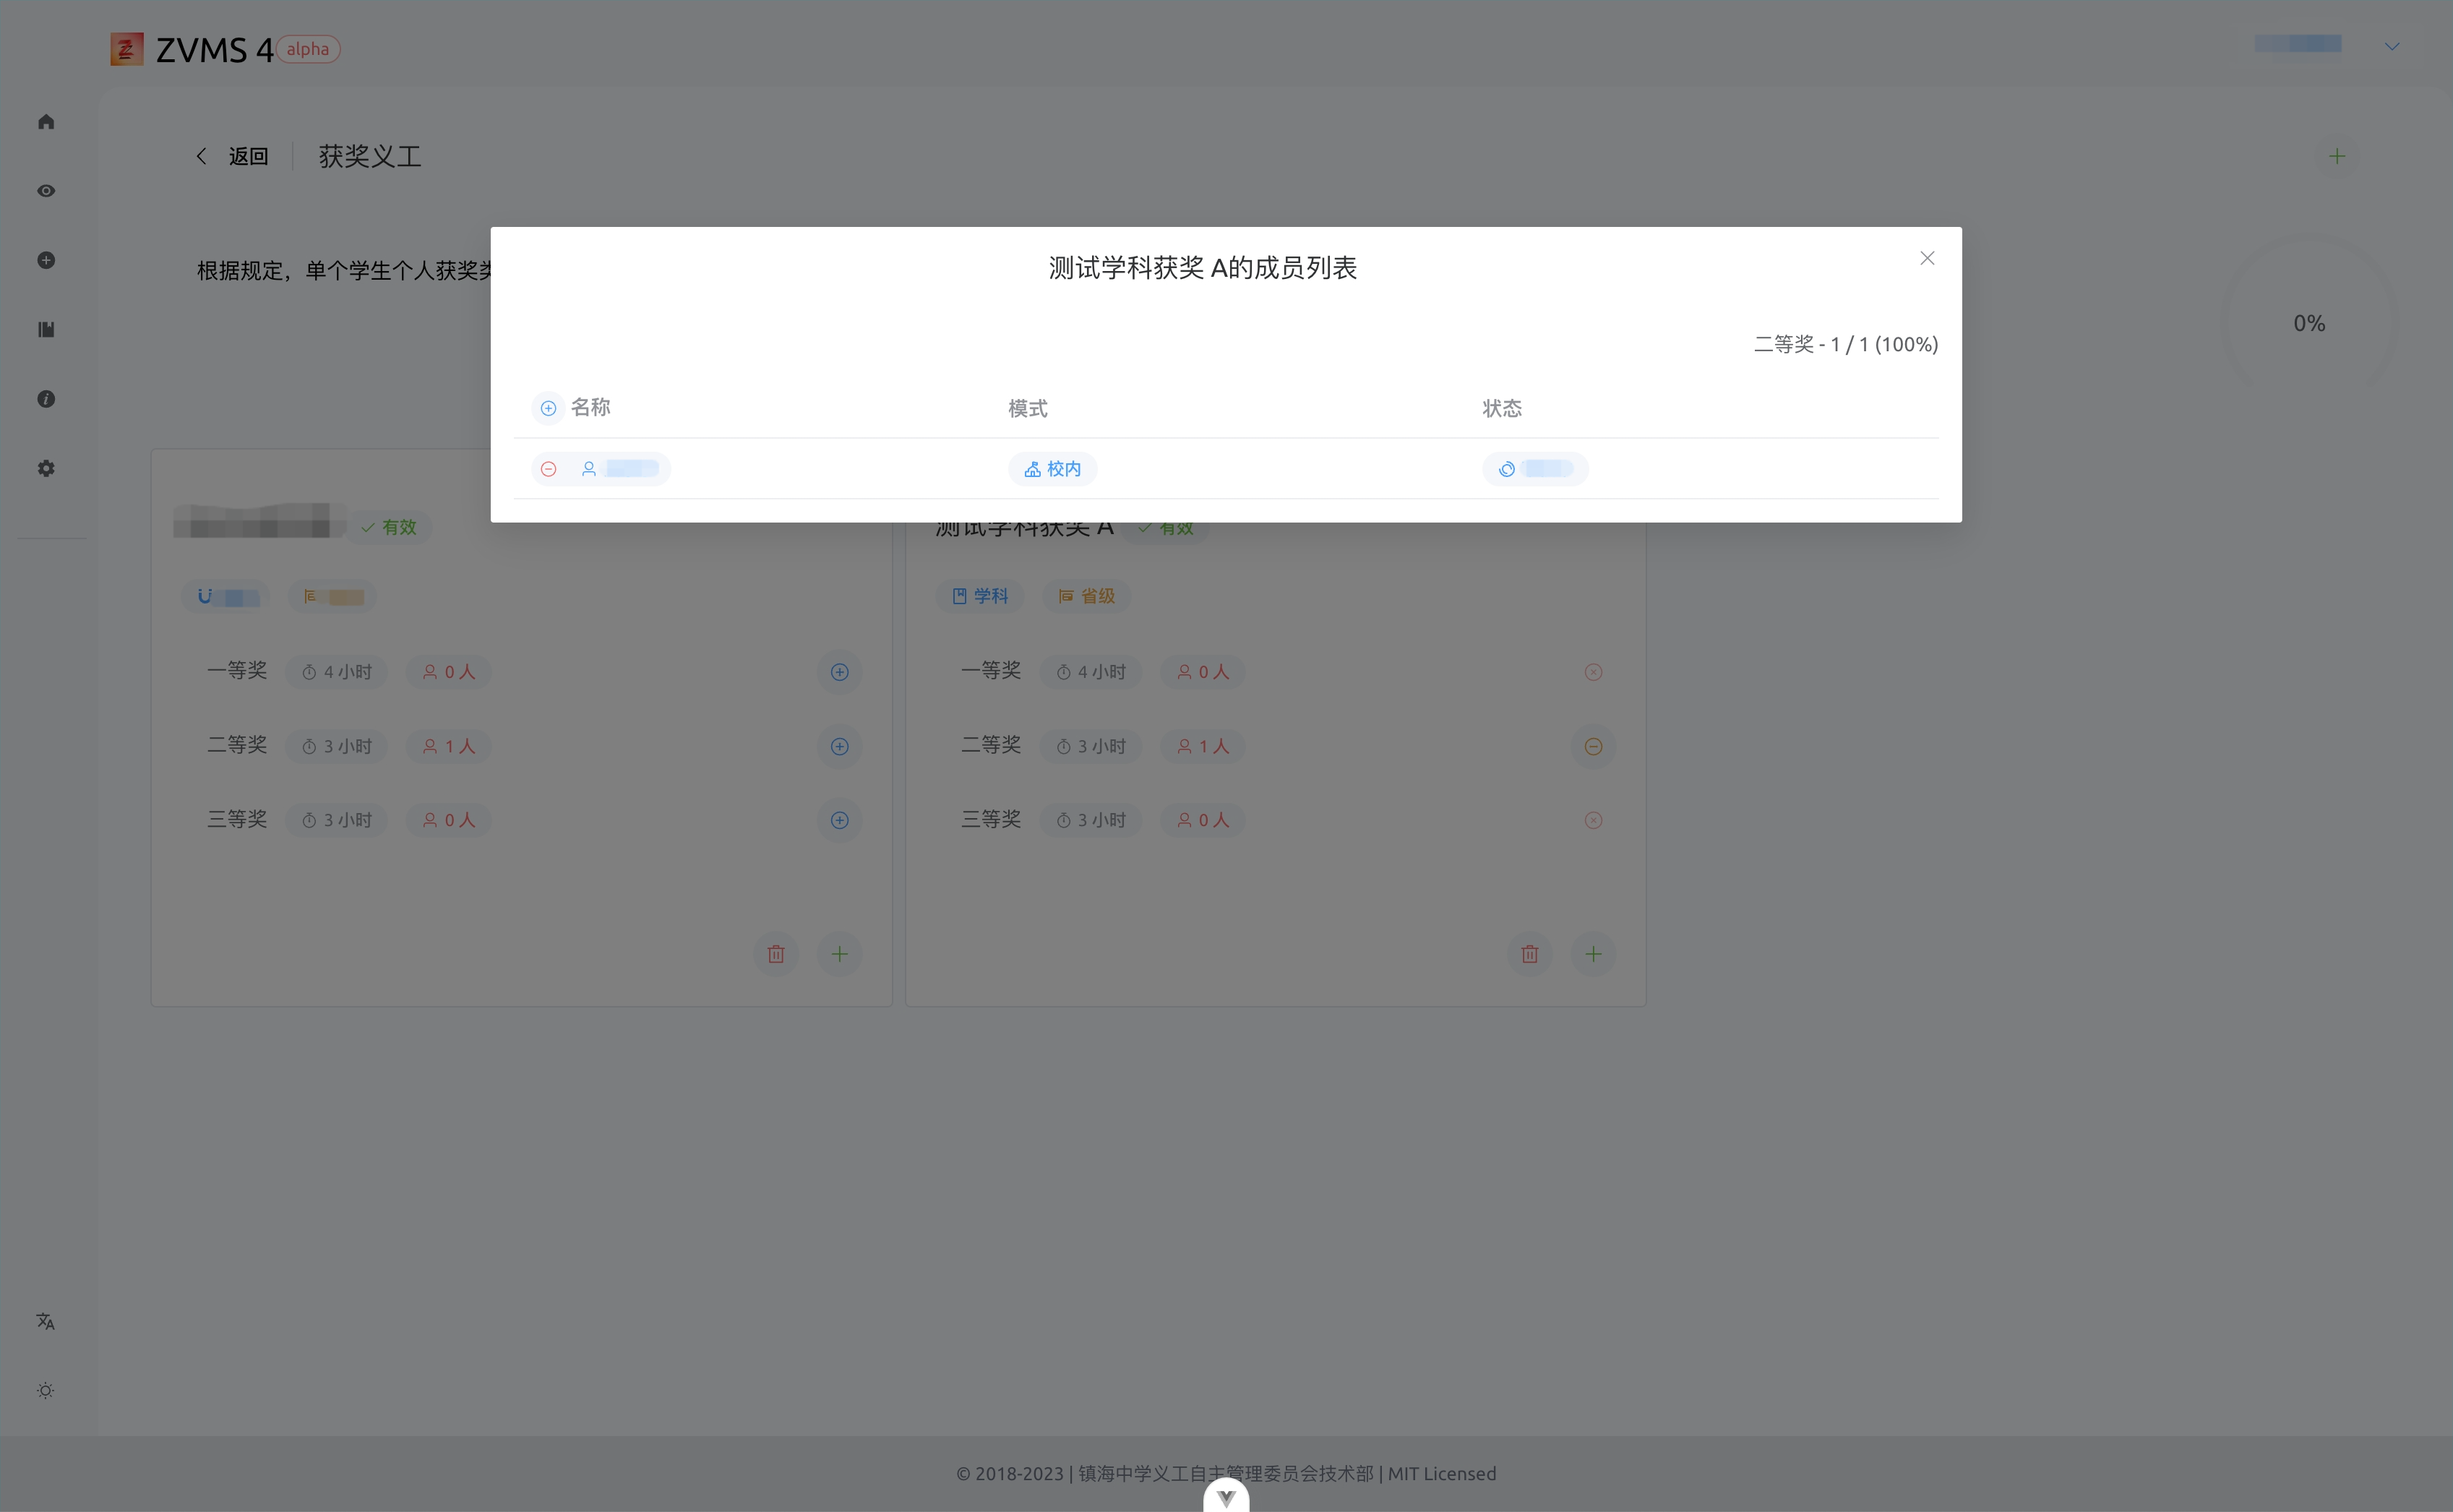
\includegraphics[width=0.8\textwidth]{../assets/image-20240303162940961.png}
  \caption{填报获奖}
  \label{fig:trophy-add-finish}
\end{figure}

当审核通过后, 时间将会自动发放. 但是请注意, 获奖义工存在上限. 系统将时间由先到后, 到达指定阈值后将不再计入时间.

\subsection{新增奖项}

具有实践部或管理员权限的账号或者具有团支书权限的账号 (需要审核) 可以添加奖项. 点击右上方的 ``+'' 即可进入创建页面.

输入基本信息后, 将会根据条件, 根据实践部文件自动创建奖项及其所对应的时间.

\begin{figure}[H]
  \centering
  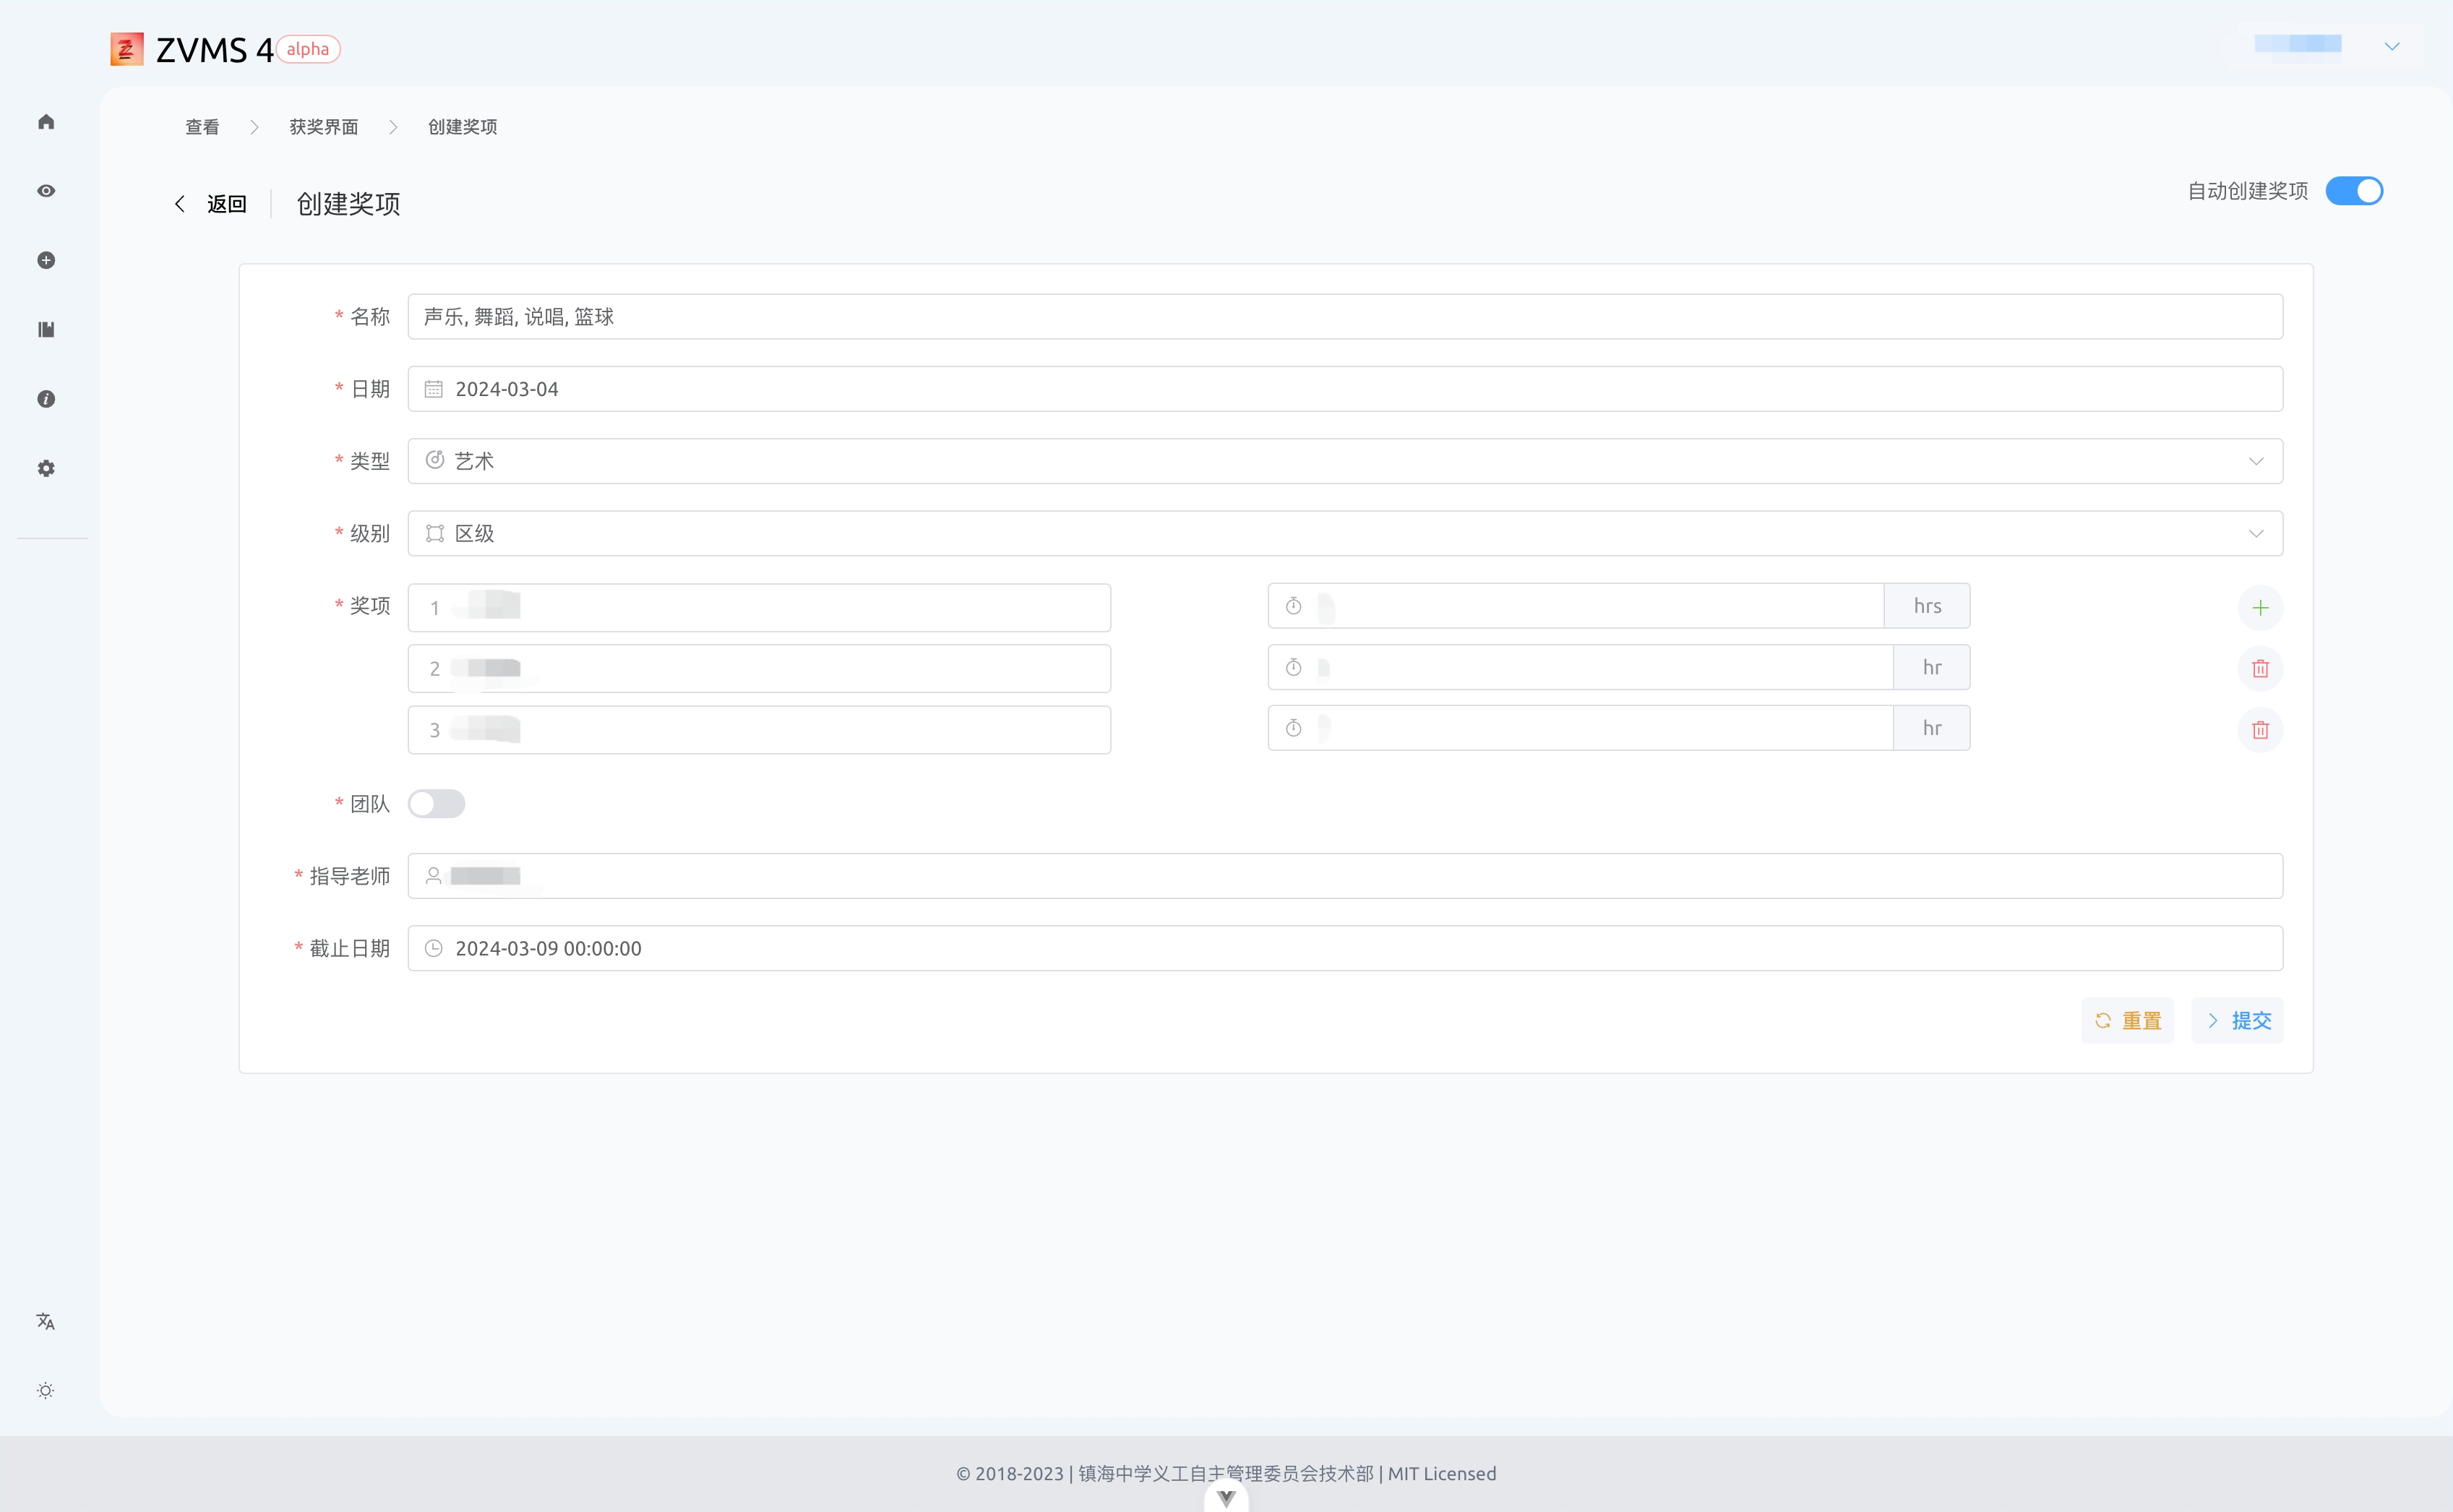
\includegraphics[width=0.8\textwidth]{../assets/image-20240303163408089.png}
  \caption{新增奖项}
  \label{fig:trophy-add-new}
\end{figure}

值得一提的是, 类型的图标将会根据名称中包含的信息自动更改.

\begin{figure}[H]
  \centering
  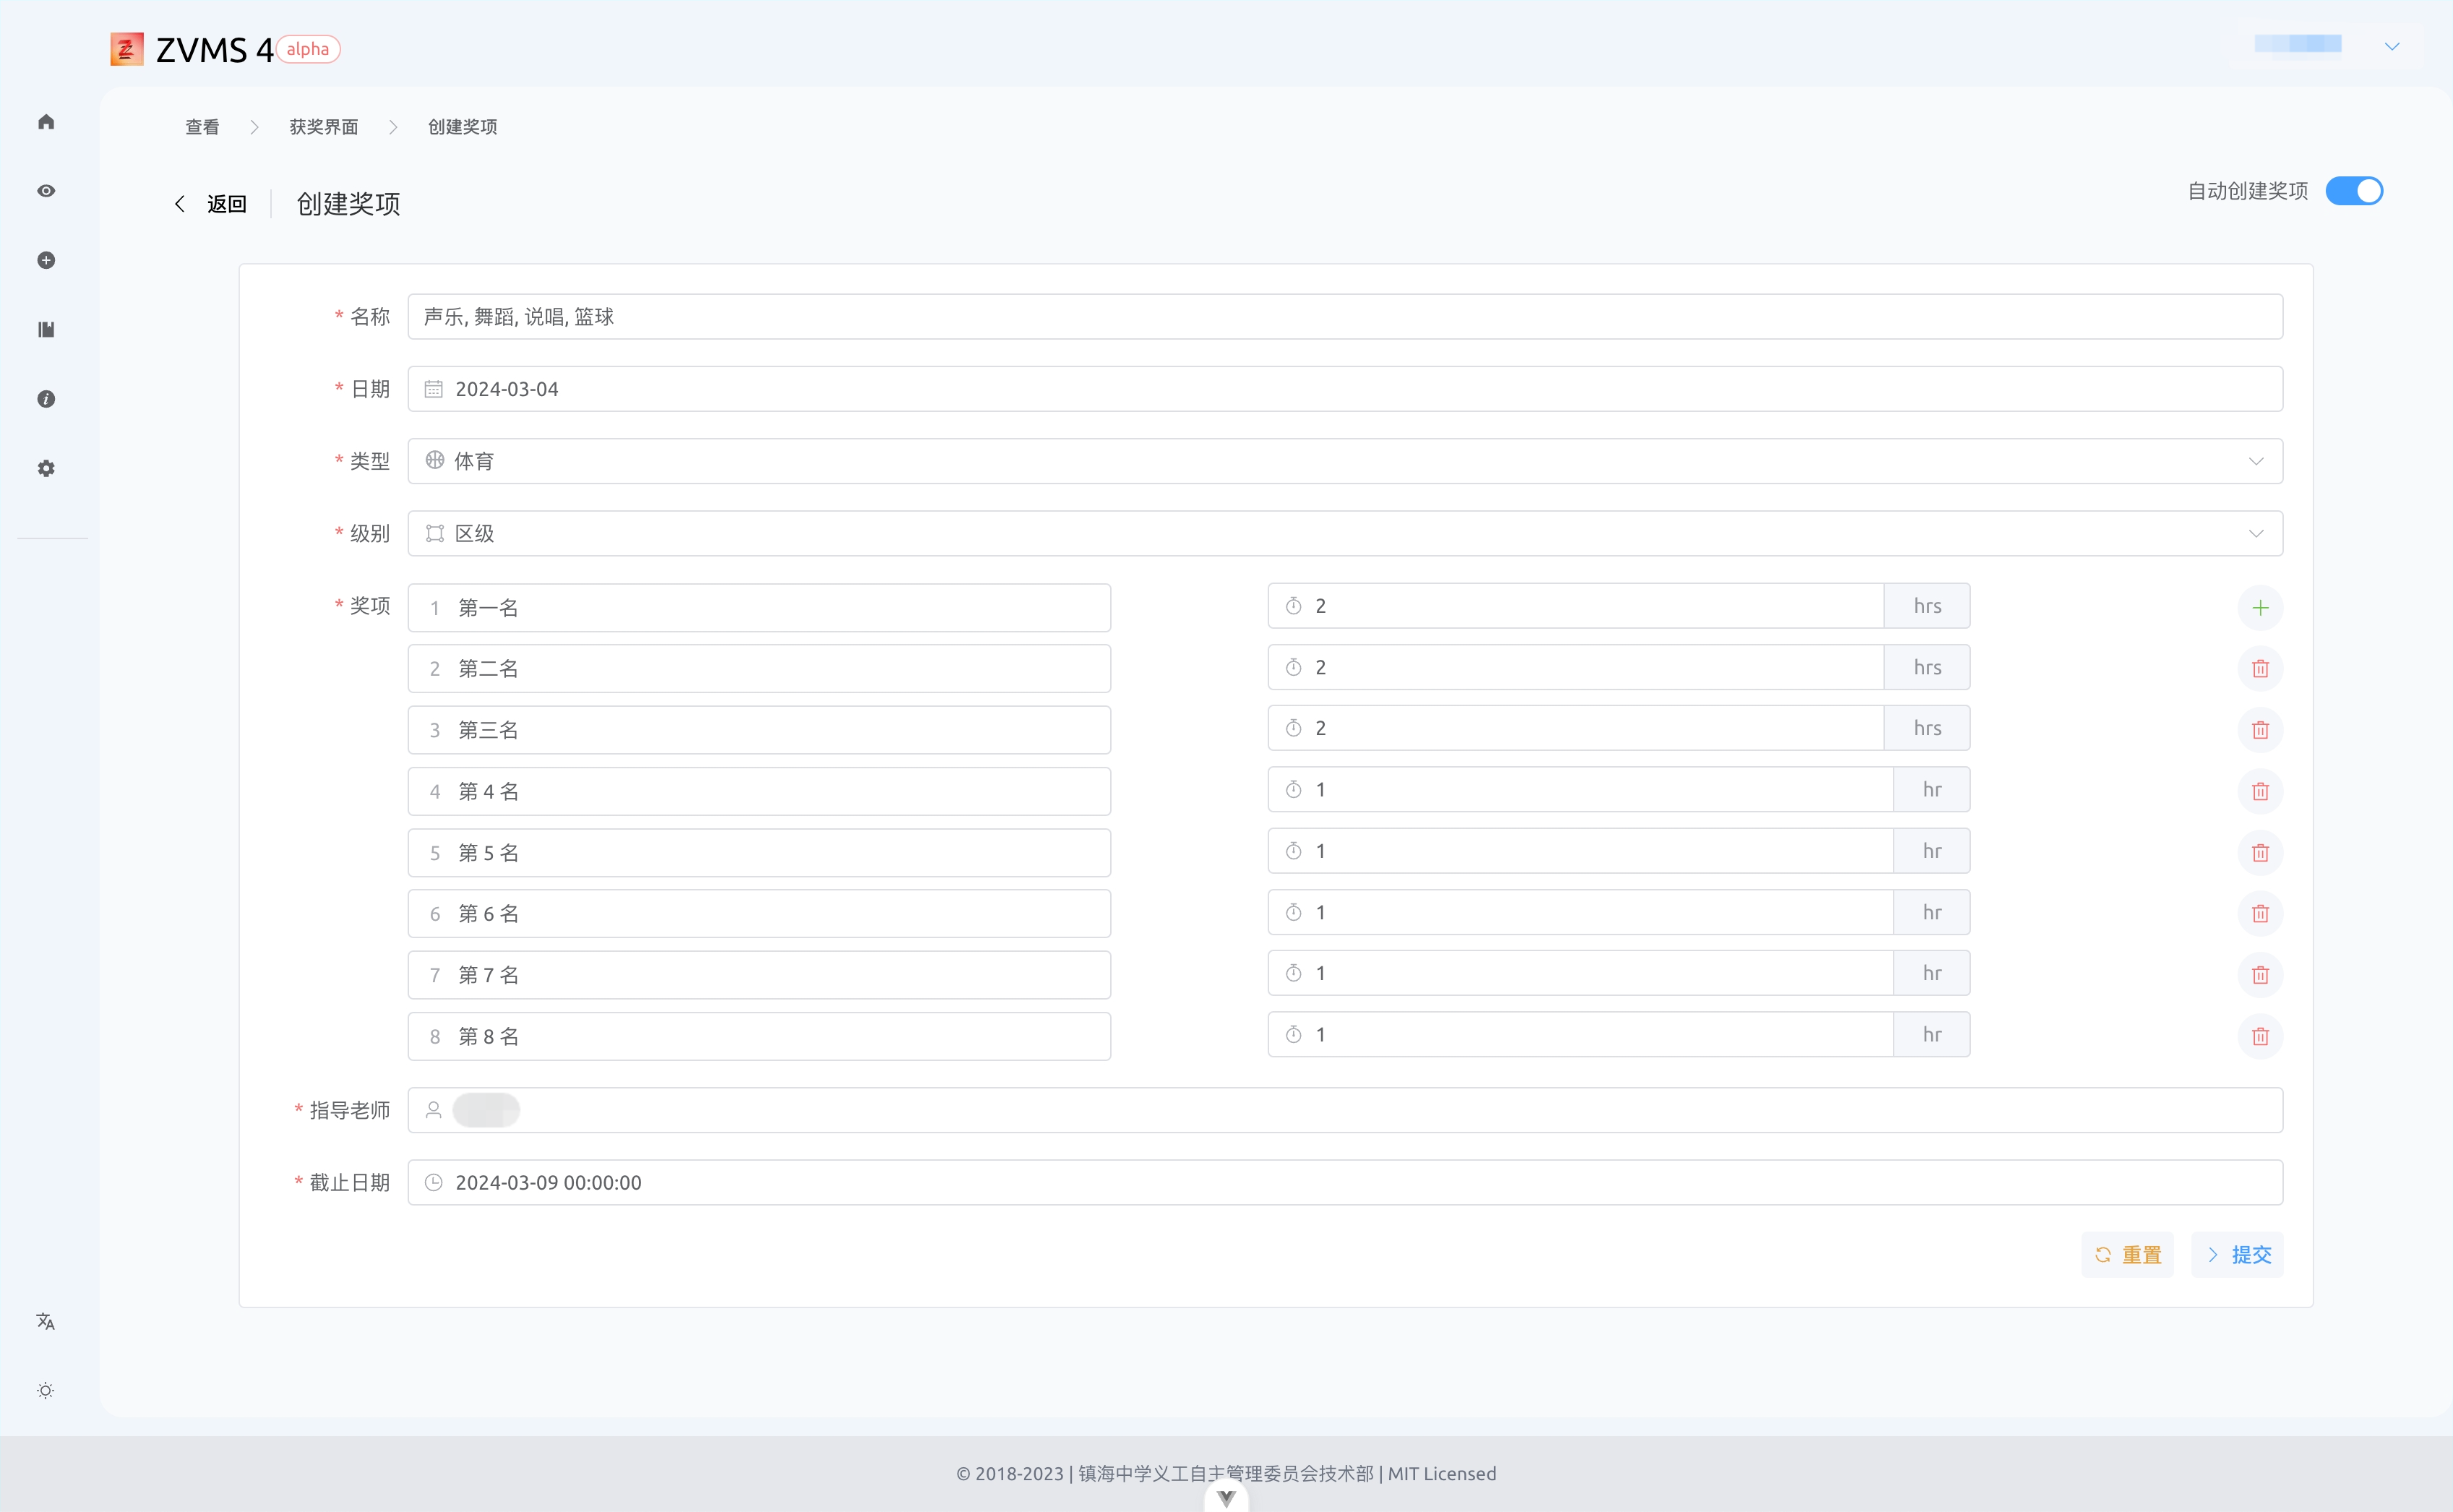
\includegraphics[width=0.8\textwidth]{../assets/image-20240303163528095.png}
  \caption{新增奖项}
  \label{fig:trophy-add-new-icon}
\end{figure}

在获奖卡片中, 您也可以添加奖项或删除奖项.

\subsection{创建义工}

ZVMS 的义工种类有 4 种:

\begin{table}[H]
  \centering
  \begin{tabular}{ccccc}
    \hline
    \textbf{类型} & \textbf{模式} & \textbf{需要审核的权限} & \textbf{完全管理权限} & \textbf{备注} \\
    \hline
    指定义工 & 校内义工 & 团支书 & 实践部 & 允许招募 \\
    社会义工 & 校外义工 & 学生 & 团支书 & 需要上传图片 \\
    实践义工 & 社会实践 & 学生 & 团支书 & 非持续开放 \\
    特殊义工 & 任意 & 不同子类分情况 & 管理员 & 特殊流程 \\
    \hline
  \end{tabular}
  \caption{义工种类}
  \label{tab:volunteer-type}
\end{table}

在创建义工处, 选择需要创建的义工.

\begin{figure}[H]
  \centering
  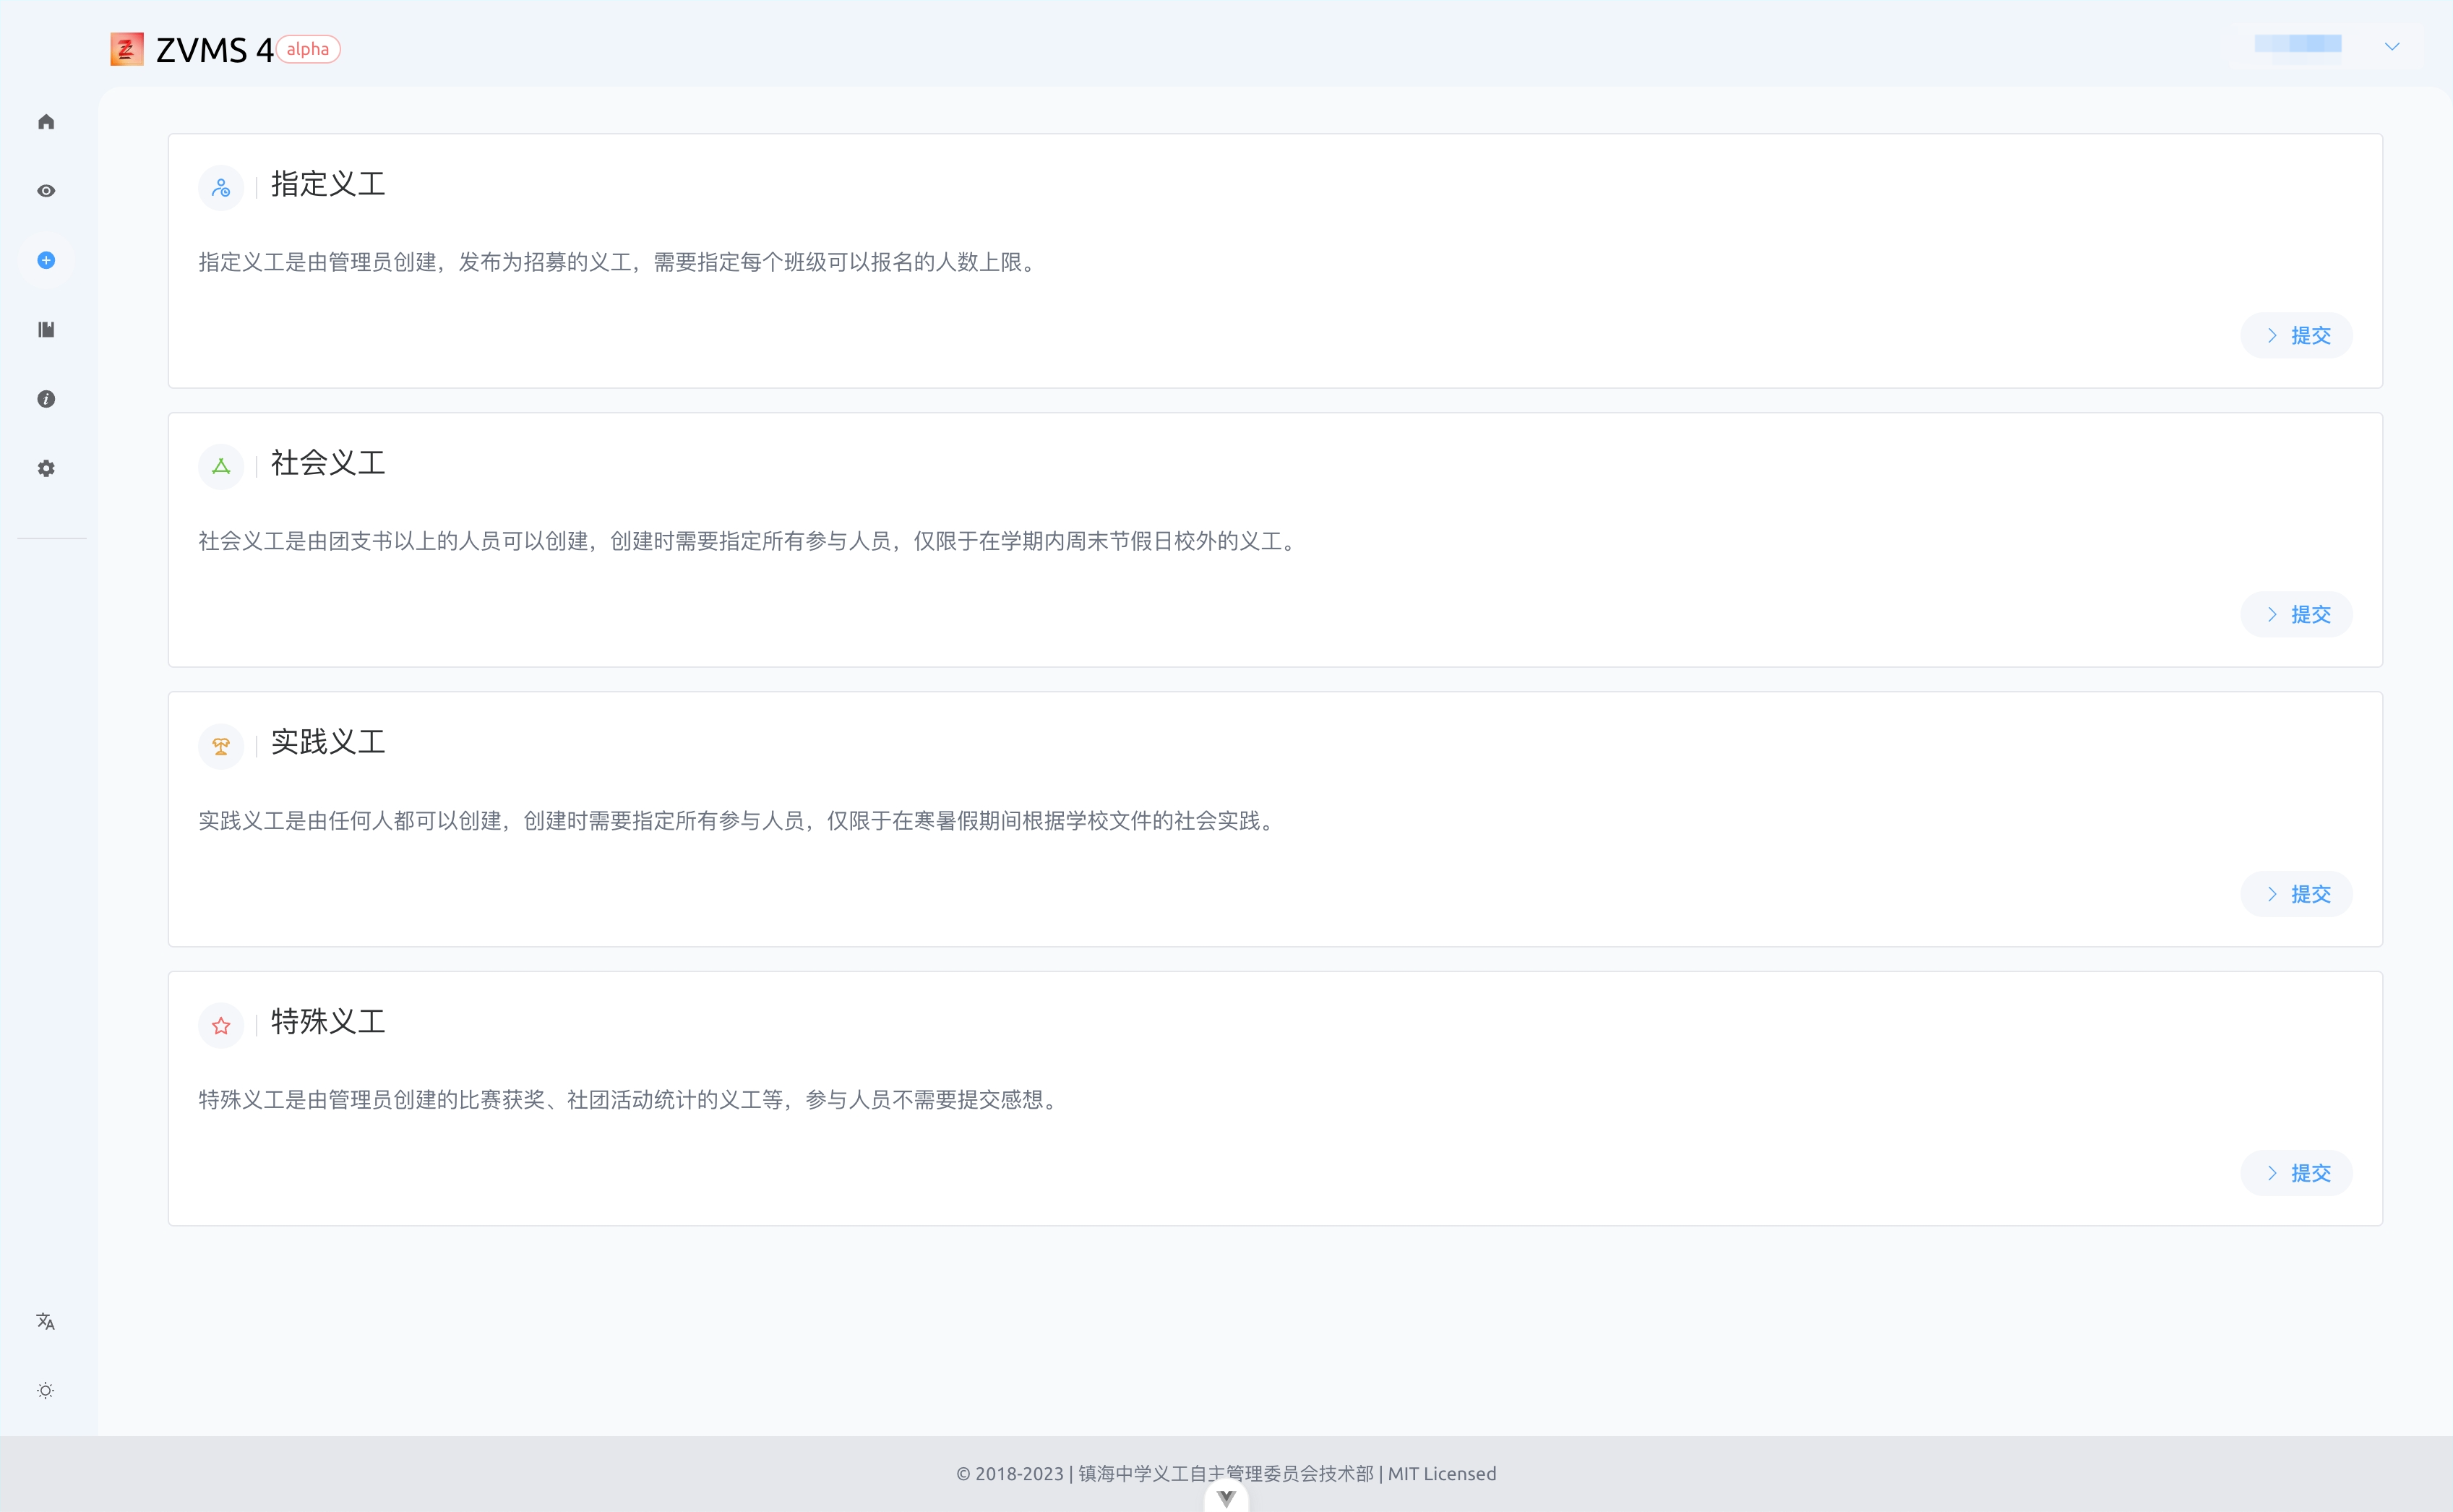
\includegraphics[width=0.8\textwidth]{../assets/image-20240303164004927.png}
  \caption{创建义工}
  \label{fig:volunteer-create}
\end{figure}

跳转到相应位置后, 填写相关信息即可提交. 值得一提的是, 您可以使用姓名或学号检索.

\begin{figure}[H]
  \centering
  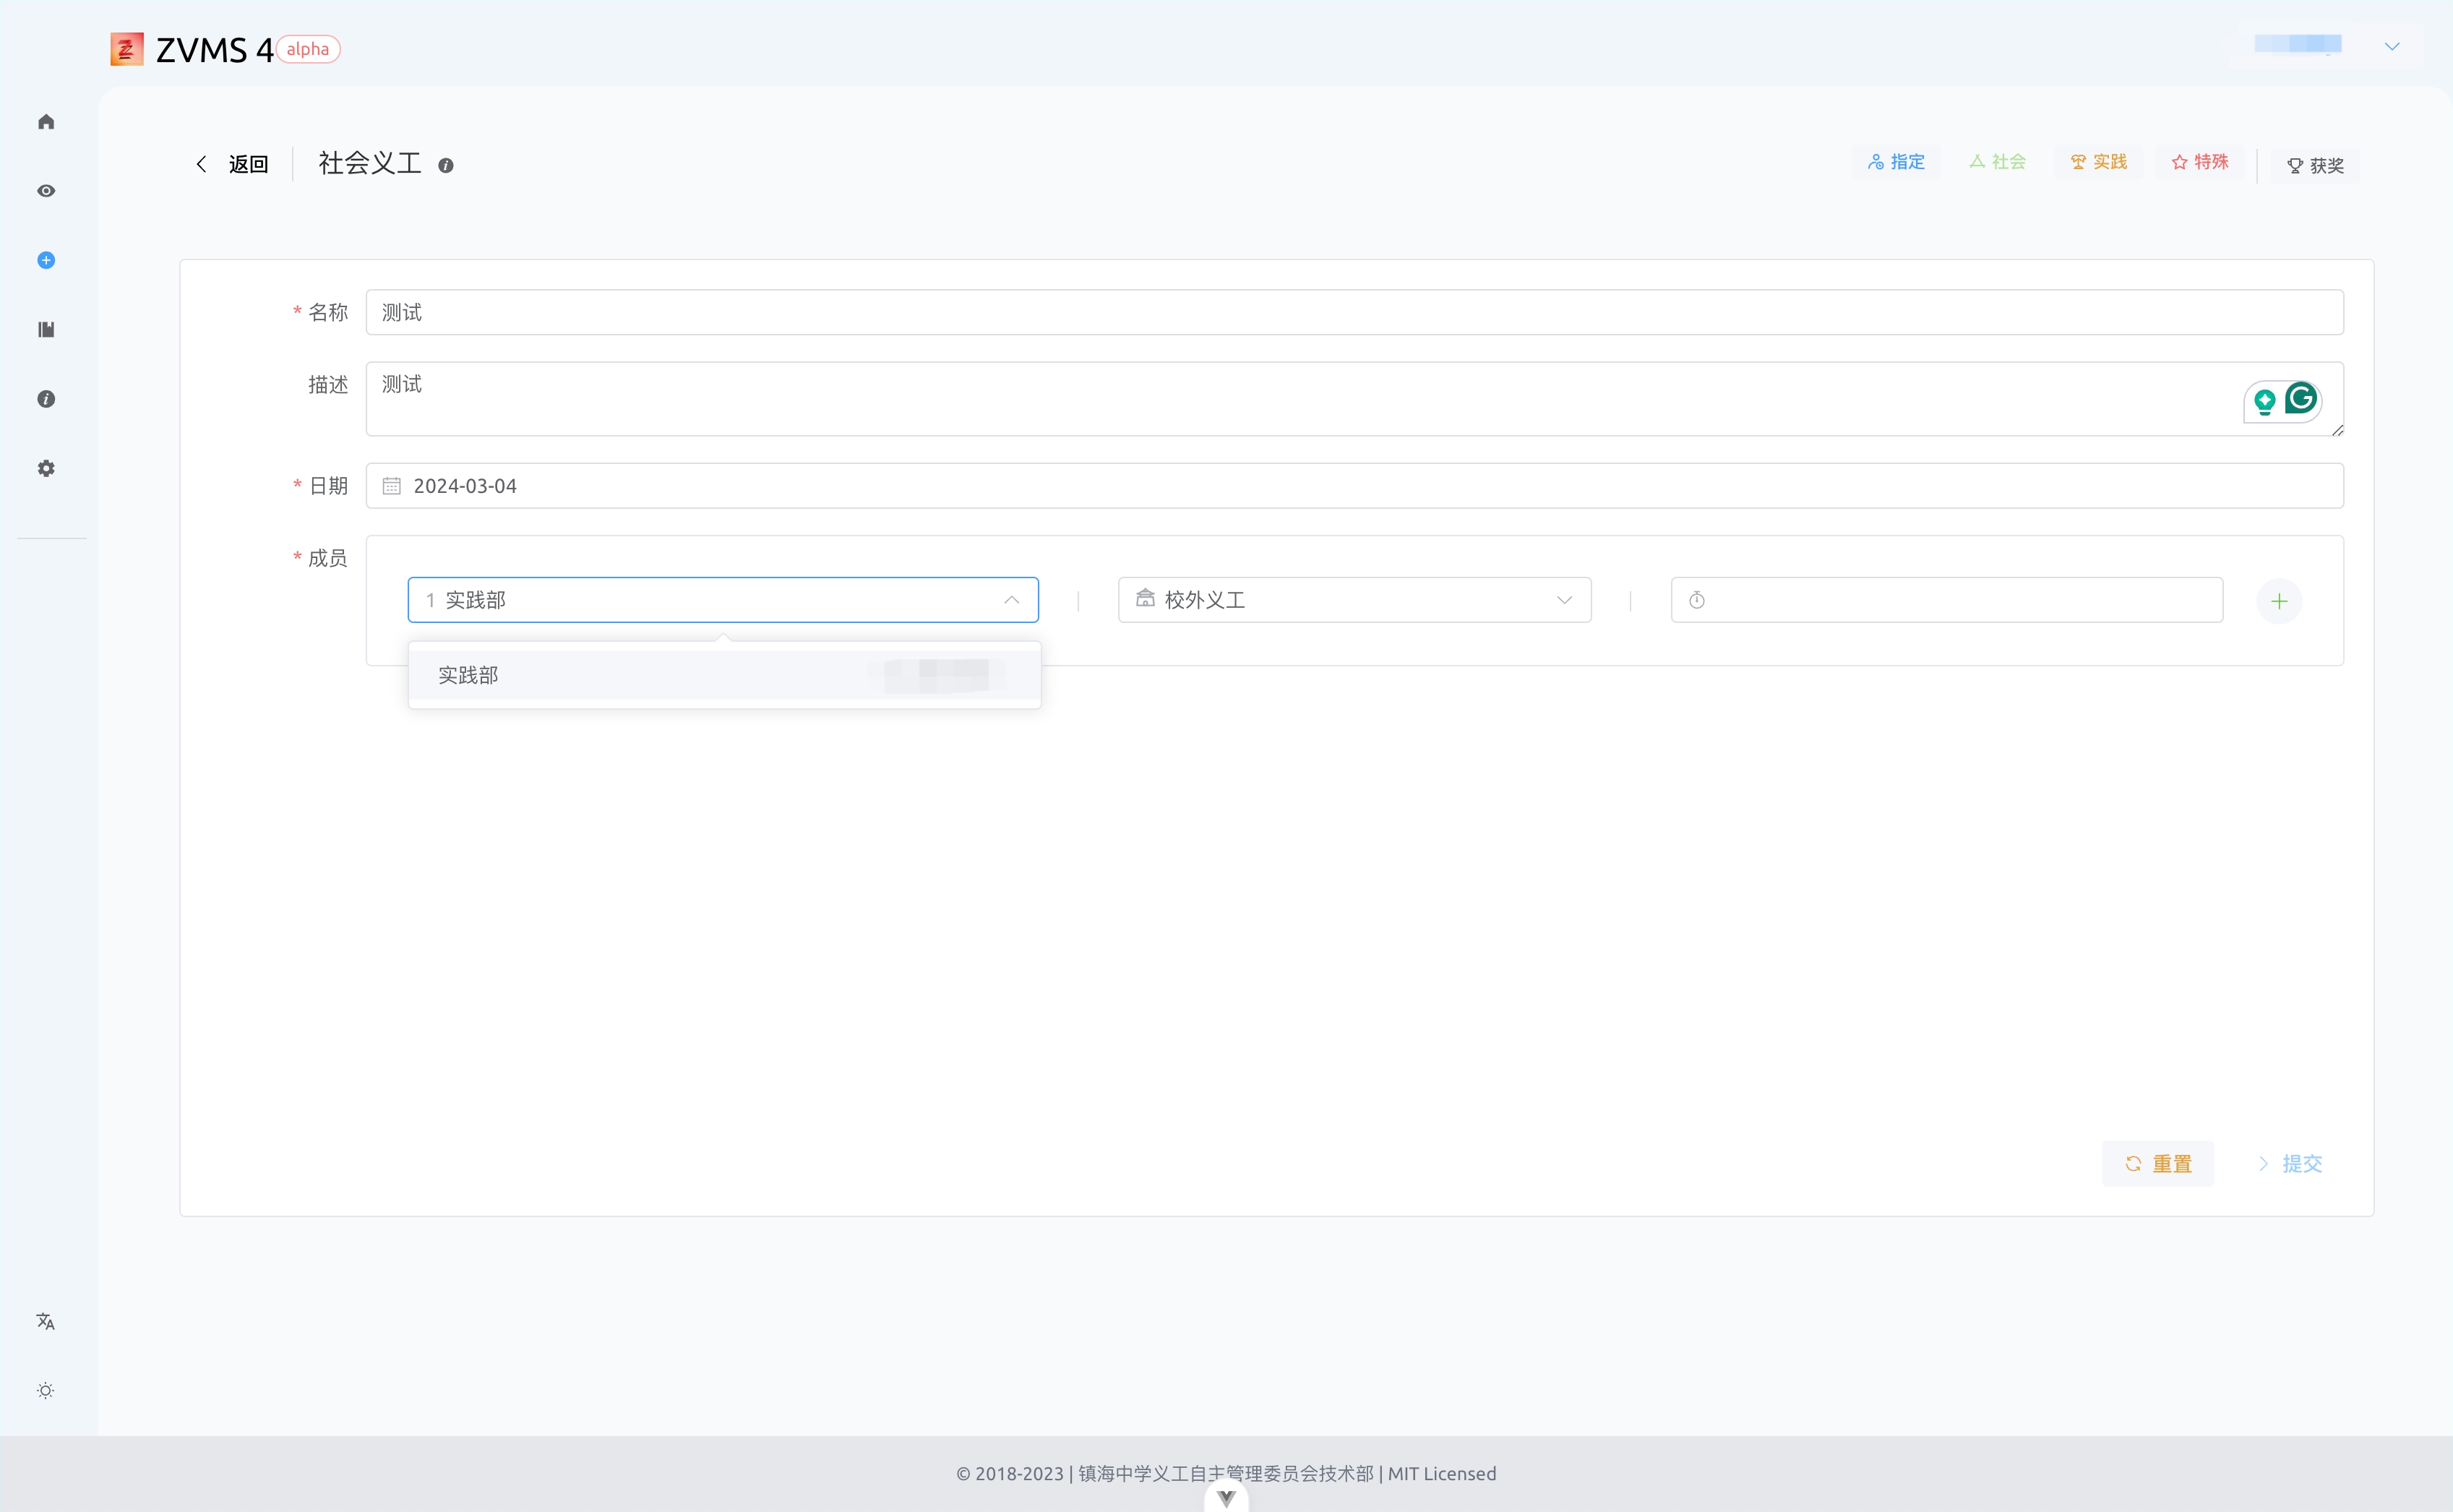
\includegraphics[width=0.8\textwidth]{../assets/image-20240303164108600.png}
  \caption{创建义工}
  \label{fig:volunteer-create-search}
\end{figure}

当表单验证有效后, 提交按钮将会启用. 提交后, 将自动跳转到相关界面.

\section{通知中心}

\label{sec:notification}

通知中心可以用来发送相关通知, 提示等.

\begin{figure}[H]
  \centering
  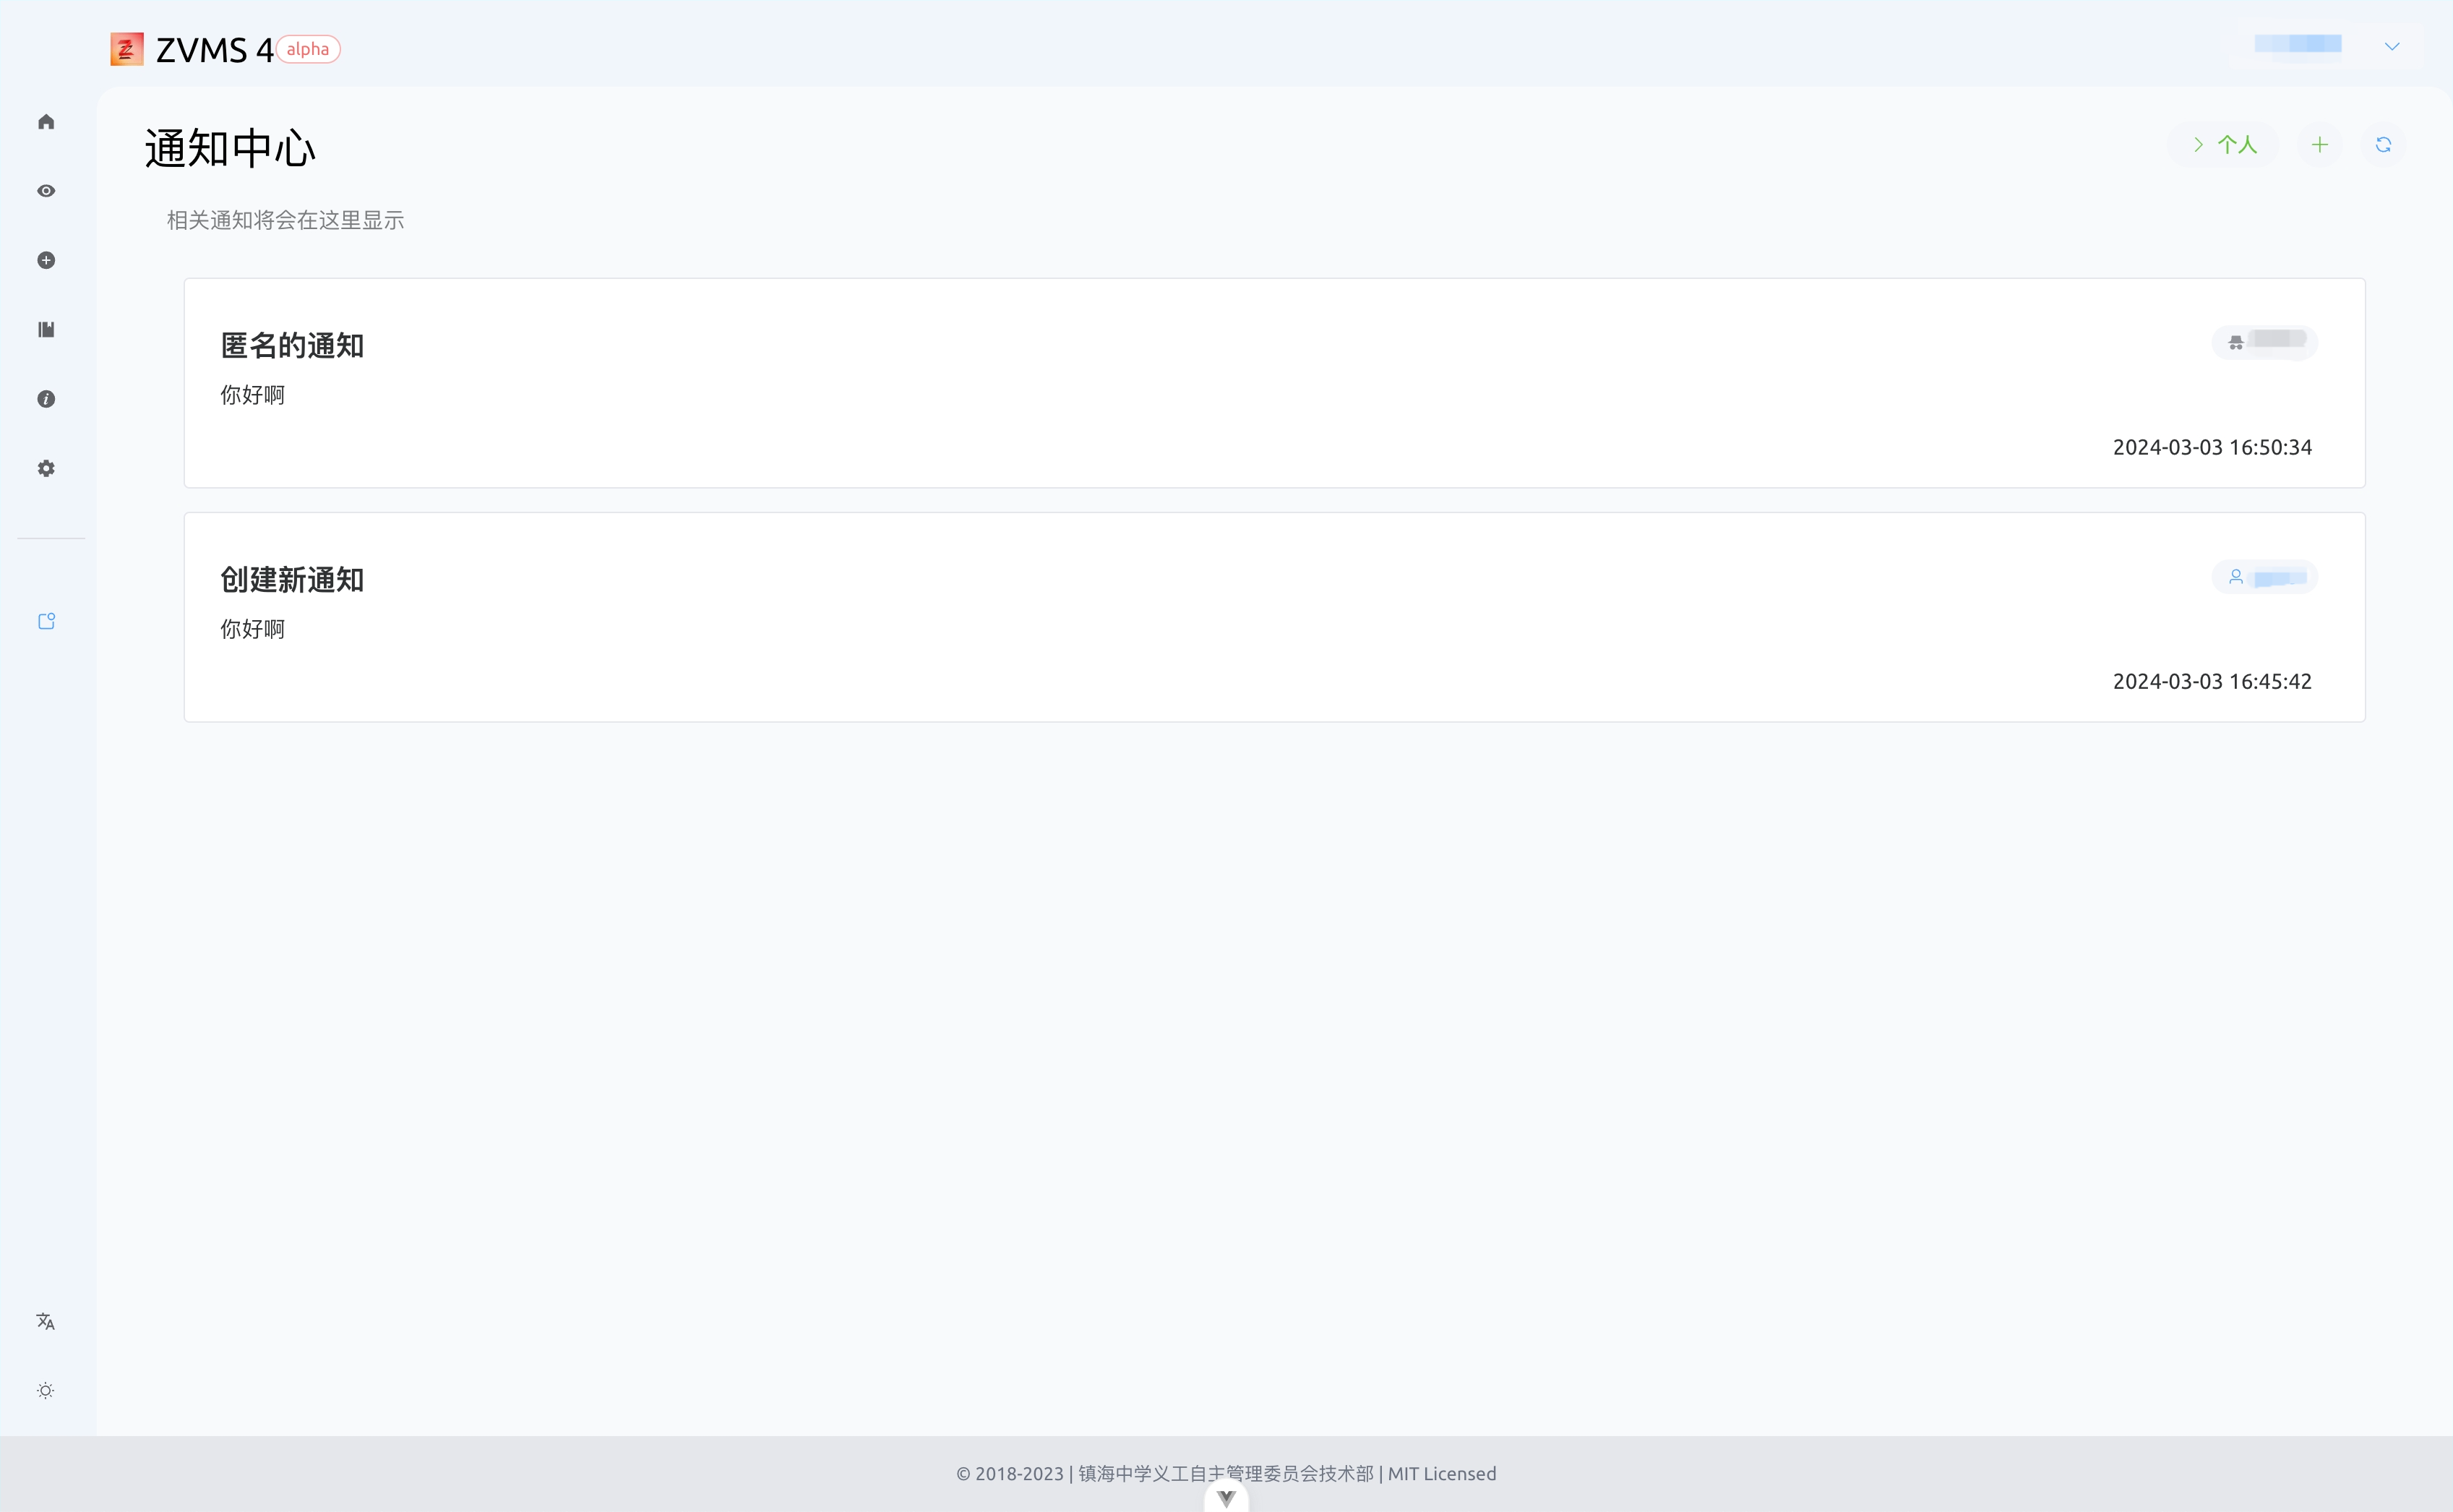
\includegraphics[width=0.8\textwidth]{../assets/image-20240303165112077.png}
  \caption{通知中心}
  \label{fig:notification}
\end{figure}

通知允许匿名发送, 但是管理员仍然可以查看发送者. 若账号不具有管理员权限, 则会显示 `匿名'. 若具有则仍然显示原来的信息, 且图标为匿名图标.

\subsection{创建通知}

点击通知中心右上角的 ``+'' 即可跳转到创建通知页面.

\begin{figure}[H]
  \centering
  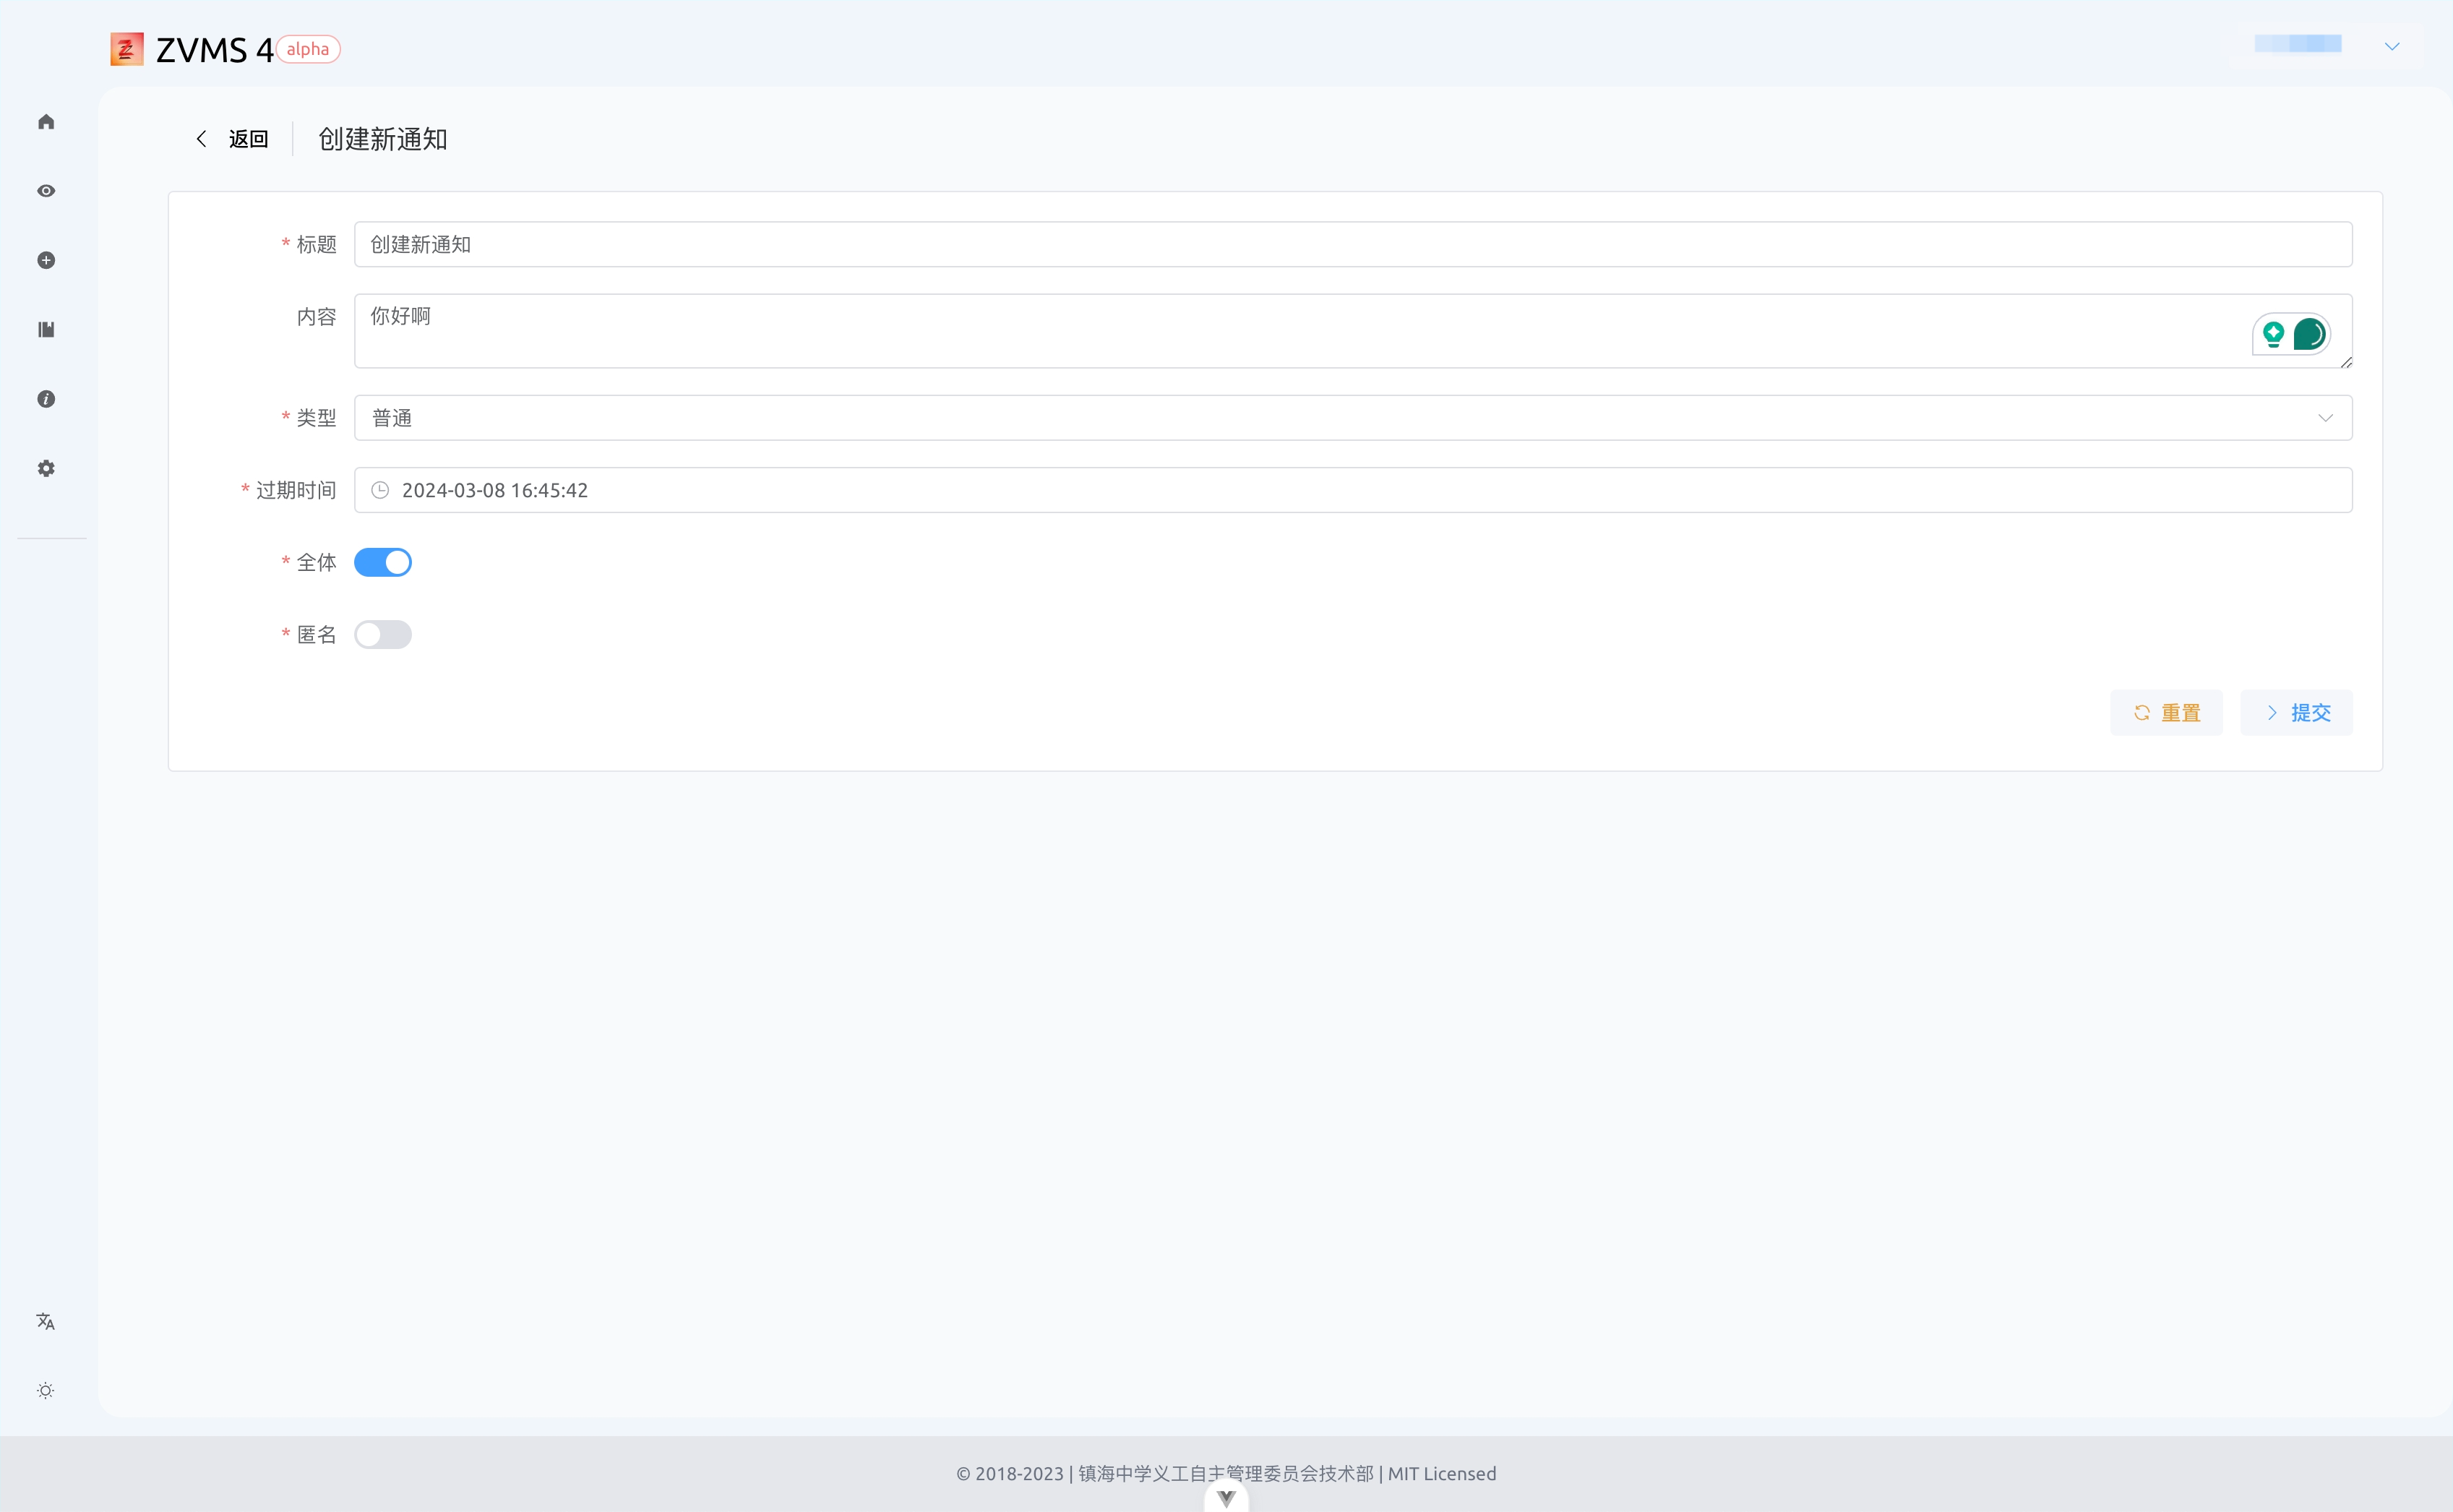
\includegraphics[width=0.8\textwidth]{../assets/image-20240303164619976.png}
  \caption{创建通知}
  \label{fig:notification-create}
\end{figure}

\end{document}
